\documentclass[12pt,fleqn,a4paper]{report}
\usepackage[many]{tcolorbox}
\usepackage{times}
\usepackage{pdflscape}
\usepackage[utf8]{inputenc}
\usepackage[T1]{fontenc}
\usepackage[french]{babel}
\usepackage{array,multirow,makecell}
\setcellgapes{1pt}
\makegapedcells
\newcommand{\chaptertoc}[1]{\chapter*{#1}
\addcontentsline{toc}{chapter}{#1}
\markboth{{#1}}{{#1}}}
\usepackage{amsmath}
\usepackage{amssymb}
\usepackage{rotating}
\usepackage{longtable}
\usepackage{amsthm}
\usepackage{makeidx}
\usepackage{listings}
\usepackage{fancybox}
\usepackage{pifont}
\usepackage{hyperref}
\usepackage[table,xcdraw]{xcolor}
\usepackage[normalem]{ulem}
\useunder{\uline}{\ul}{}
\usepackage{ragged2e}

% ====== BIBLIOGRAPHY: biblatex ONLY (supprime natbib) ======
\usepackage[style=numeric,backend=biber]{biblatex}
\addbibresource{bbbib.bib}
% ===========================================================

\definecolor{main}{HTML}{5989cf}
\definecolor{sub}{HTML}{cde4ff}
\makeatletter
\newcommand\blankpage{%
    \null
    \thispagestyle{empty}%
    \addtocounter{page}{-1}%
    \newpage}
\makeatother
\tcbset{
    sharp corners,
    colback = white,
    before skip = 0.2cm,
    after skip = 0.5cm
}
\newtcolorbox{boxI}{
    colback = sub,
    colframe = main,
    boxrule = 0pt,
    toprule = 6pt
}

\usepackage{titlesec}
\titleformat{\chapter}[display]
{\normalfont\huge\bfseries}{\chaptertitlename\ \thechapter}{20pt}{\Huge}

\usepackage{fancyhdr}
\usepackage{epsfig}
\usepackage{epstopdf}
\usepackage{subfig}
\usepackage{multirow}
\usepackage{algorithm}
\usepackage{algorithmic}
\usepackage[francais]{minitoc}
\mtcselectlanguage{french}
\setcounter{minitocdepth}{1}
\usepackage{graphicx}
% Tous les fichiers images (logos + captures + diagrammes) sont cherchés
% automatiquement dans ces trois dossiers : plus besoin de prefixer chaque
% \includegraphics avec son chemin complet.
\graphicspath{{Image/}{images/}{rapport_diagrams/}}
\usepackage{tabularx}
\usepackage{booktabs}
\usepackage{fancyvrb}
\setcounter{secnumdepth}{4}
\setcounter{tocdepth}{4}
\usepackage{latexsym}
\usepackage{calc}
\usepackage{lettrine}
\usepackage{a4wide}
\usepackage{verbatim}
\usepackage{moreverb}
\usepackage{pdfpages}
\usepackage{float}
\usepackage{caption}
\usepackage{longtable}
\captionsetup{position=below}
\newcolumntype{R}[1]{>{\raggedleft\arraybackslash }b{#1}}
\newcolumntype{L}[1]{>{\raggedright\arraybackslash }b{#1}}
\newcolumntype{C}[1]{>{\centering\arraybackslash }b{#1}}
\renewcommand{\baselinestretch}{1.1}
\setlength{\parskip}{0.3cm}
\usepackage{color}

\usepackage[Lenny]{fncychap}
\ChTitleVar{\Huge\sffamily\bfseries}

\newtheorem{Theorem}{Theorem}[chapter]
\newtheorem{Example}{Example}[chapter]
\newtheorem{c-Example}{Counter-example}[chapter]
\newtheorem{Proposition}{Proposition}[chapter]
\newtheorem{Definition}{Definition}[chapter]
\newtheorem{Lemma}{Lemma}[chapter]
\newtheorem{Corol}{Corollary}[chapter]

\vfuzz2pt
\hfuzz2pt

\colorlet{LightRubineRed}{red!70!}
\colorlet{Mycolor1}{blue!40!black!60!}

\pagestyle{fancy}
\fancyhead[LO,RE]{\textsl{\rightmark}}
\renewcommand{\headrulewidth}{0.4pt}
\renewcommand{\chaptermark}[1]%
{\markboth{\itshape{Chapter~\thechapter~: \ #1}}{}}
\renewcommand{\sectionmark}[1]%
{\markright{\itshape{Section~\thesection~--~\ #1}}}
\lhead[\thepage]{\leftmark}
\rhead[\leftmark]{\thepage}

\begin{document}
\dominitoc
\justifying
\begin{justify}

% ==========================================================================
% PAGE DE GARDE — refaite (spécialité, nom de l'application, mémoire, jury)
% Champs à vérifier / corriger : marqués par un commentaire "% VERIFIER:"
% ==========================================================================
\thispagestyle{empty}
\begin{figure}[]
\begin{minipage}[l]{.3\textwidth}
\begin{center}
\flushleft 
\includegraphics[width=3cm]{univk.jpg}
\end{center}
\end{minipage}
\begin{minipage}{.36\textwidth}
\begin{center}
\footnotesize{République Tunisienne
Ministère de l'Enseignement Supérieur, de
la Recherche Scientifique et de la
Technologie }
\noindent
{\color{Mycolor1} \rule{\linewidth}{0.5mm} }
\footnotesize{Université de Kairouan
Institut Supérieur d'Informatique et de
Gestion de Kairouan }
\end{center}
\end{minipage}
\begin{minipage}{.32\textwidth}
\begin{center}
\flushright 
\includegraphics[width=4cm]{isigk.png}
\end{center}
\end{minipage}
\end{figure}

\vspace{0.3cm}
\begin{center}
\noindent
{\color{Mycolor1} \rule{\linewidth}{0.5mm} }\\[0.3cm]
\Large{\textbf{\textit{MÉMOIRE DE PROJET DE FIN D'ÉTUDES}}}\\[0.15cm]
% VERIFIER: intitulé exact du diplôme et de la spécialité (ISIGK / Université de Kairouan)
\large{Présenté en vue de l'obtention du diplôme de}\\[0.1cm]
\large{\textbf{Mastère Professionnel en Réseaux et Applications Distribuées}}\\[0.4cm]
{\color{Mycolor1} \rule{\linewidth}{1mm} }\\[0.3cm]
{\huge \textbf{AMANA}} \\[0.2cm]
% VERIFIER: sous-titre — reformuler si besoin
{\normalsize \textit{Plateforme mobile et web multiservices de livraison~: repas, courses, colis entre particuliers et paiement de factures}}\\[0.2cm]
\noindent
{\color{Mycolor1} \rule{\linewidth}{1mm} }\\[0.4cm]

\Large{Élaboré par~: \textit{Adam Cherif}}\\[0.3cm]
% VERIFIER: nom de l'encadreur académique
\large{\textbf{Encadré par~: Mme Olfa Harrabi}}
\end{center}

\vspace{0.6cm}
\noindent
{\color{Mycolor1} \rule{\linewidth}{0.5mm} }
\vspace{0.4cm}

\begin{center}
% VERIFIER: composition du jury (à compléter par l'étudiant avant l'impression finale)
\begin{tabular}{ll}
Président du jury~: & \makebox[6cm]{\hrulefill} \\[0.35cm]
Rapporteur~: & \makebox[6cm]{\hrulefill} \\[0.35cm]
Encadreur~: & Mme Olfa Harrabi \\
\end{tabular}

\vspace{0.6cm}
% VERIFIER: date de soutenance
Soutenu le~: \makebox[4cm]{\hrulefill}

\vspace{0.6cm}
Année universitaire~: 2025 / 2026
\end{center}

\tableofcontents
\newpage

\thispagestyle{empty}

\vspace*{2cm}

\begin{center}
  \rule[0.5ex]{3.2cm}{0.5pt} \quad {\Huge \textbf{Remerciements}} \quad \rule[0.5ex]{3.2cm}{0.5pt}
\end{center}

\vspace{1.5cm}

\noindent \textbf{M}es remerciements s'adressent tout d'abord au bon Dieu le tout puissant et miséricordieux, qui m'a donné la force, la volonté et la patience pour accomplir ce modeste travail.

\vspace{0.8cm}

\noindent \textbf{J}e tiens à exprimer ma profonde gratitude et mes sincères remerciements à mon encadreuse académique, \textbf{Mme Olfa Harrabi}, pour son encadrement précieux, ses conseils avisés et sa disponibilité tout au long de la réalisation de ce projet.

\vspace{0.8cm}

\noindent \textbf{M}es remerciements s'adressent également aux membres du jury d'avoir accepté d'évaluer ce travail, ainsi qu'à l'ensemble du corps professoral de l'\textbf{Institut Supérieur d'Informatique et de Gestion de Kairouan (ISIGK)}.
\newpage
\thispagestyle{empty}

\vspace*{1.5cm}

\begin{center}
  \rule[0.5ex]{3.2cm}{0.5pt} \quad {\Huge \textbf{Dédicaces}} \quad \rule[0.5ex]{3.2cm}{0.5pt}
\end{center}

\vspace{1.2cm}

\begin{center}
  \noindent \textbf{À} mes chers parents, pour leurs sacrifices inestimables, leur soutien inconditionnel, leurs prières quotidiennes et leur amour infini qui ont éclairé mon parcours.

  \vspace{0.7cm}

  \noindent \textbf{À} mon cher frère, mon compagnon de route, mon guide et ma fierté, que Dieu le garde en bonne santé.

  \vspace{0.7cm}

  \noindent \textbf{À} toute mes proches, pour leurs encouragements constants et leur présence bienveillante à chaque étape.

  \vspace{0.7cm}

  \noindent \textbf{À} moi-même, en reconnaissance de la patience, de la persévérance, de la passion et des efforts soutenus investis dans la réalisation de ce projet, malgré les défis et les nuits de labeur.

  \vspace{1.1cm}

  \noindent \textbf{Q}u'ils trouvent tous dans ce modeste travail le témoignage de ma profonde affection, de mon attachement indéfectible et le fruit d'une grande détermination.
\end{center}

\newpage
\newpage

% ==========================================================================
% INTRODUCTION GÉNÉRALE — restructurée en 4 parties explicites
% ==========================================================================
\chapter*{\hfill Introduction générale \hfill}
\markboth{\small{Introduction générale}}{\small{Introduction générale}}
\addcontentsline{toc}{chapter}{Introduction générale}

\renewcommand{\thepage}{\arabic{page}}
\setcounter{page}{1}

\subsection*{Contexte général du projet}

Le téléphone intelligent a changé la façon dont les gens font leurs achats. Commander un repas, faire ses courses ou envoyer un colis sans se déplacer est devenu une habitude courante, en Tunisie comme ailleurs. Les applications de livraison répondent à ce besoin en reliant, au sein d'un même système numérique, trois acteurs qui devaient auparavant communiquer par téléphone ou en personne~: le client, le commerçant et le livreur. Ce projet s'inscrit dans ce mouvement, avec une particularité~: il vise en priorité un marché encore peu couvert par les grandes plateformes, le gouvernorat de Kairouan.

\subsection*{Présentation de l'application}

Le projet consiste à concevoir et à développer \textbf{Amana}, une plateforme de livraison multiservices composée de quatre applications~: une application mobile pour le client, une pour le livreur, une pour le commerçant partenaire, et un tableau de bord web pour l'administrateur. Le client y trouve quatre services réunis au même endroit~: la commande de repas auprès de restaurants, l'achat de produits dans des supermarchés partenaires, l'envoi de colis entre particuliers, et le paiement de factures. Un livreur assure le transport, un commerçant gère son catalogue et ses commandes, et un administrateur supervise l'ensemble depuis un tableau de bord.

\subsection*{Objectifs du projet}

L'objectif principal est de simplifier, pour un client de Kairouan, l'accès à plusieurs services du quotidien depuis une seule application, plutôt que d'en installer une par besoin. Pour le commerçant, l'objectif est de lui donner un outil de gestion clair, sans dépendre d'un intermédiaire externe coûteux. Pour le livreur, il s'agit d'offrir un moyen simple de recevoir des missions et de suivre ses revenus. Enfin, pour l'administrateur, l'objectif est de disposer d'une vue d'ensemble fiable de l'activité, pour intervenir rapidement en cas de besoin.

\subsection*{Organisation du mémoire}

Ce mémoire est organisé en cinq chapitres. Le chapitre~1, \textit{Cadre du projet et expression des besoins}, présente le contexte, les services proposés, l'analyse des solutions déjà présentes sur le marché tunisien, et le cahier des charges qui en découle. Le chapitre~2, \textit{Analyse et conception du système}, modélise le fonctionnement de la plateforme à travers les diagrammes UML de cas d'utilisation, de classes et de séquence. Le chapitre~3, \textit{Réalisation technique}, détaille les technologies utilisées, l'organisation du code, l'implémentation du back-end, la sécurité et l'intégration de l'intelligence artificielle. Le chapitre~4, \textit{Présentation des applications et des interfaces}, montre concrètement les quatre applications et leurs écrans. Le chapitre~5, \textit{Tests, déploiement et maintenance}, décrit les tests effectués, l'état du déploiement et les pistes de maintenance envisagées. Une conclusion générale referme le document.

%************CHAP1***********
\chapter{Cadre du projet et expression des besoins}

\section{Présentation générale du projet}

Amana est une plateforme de livraison pensée pour le marché tunisien, avec un point de départ précis~: le gouvernorat de Kairouan, une région où les grandes applications internationales et les principales applications tunisiennes ne sont pas présentes. Plutôt que de se limiter à un seul service, comme le font la plupart des applications existantes, Amana réunit quatre services dans une seule plateforme~: la commande de repas, l'achat de produits de supermarché, l'envoi de colis entre particuliers et le paiement de factures. Ce chapitre présente le contexte de ce choix, les services proposés, l'étude des solutions déjà présentes sur le marché, puis le cahier des charges qui a guidé la conception du système.

\section{Contexte et enjeux du projet}

Le paysage de la consommation en Tunisie change rapidement, porté par l'usage quotidien des téléphones intelligents et par le besoin de gagner du temps. Commander un repas ou acheter des produits de première nécessité sans se déplacer est devenu une habitude pour de nombreux Tunisiens, surtout dans les grandes villes. Ce projet part d'un constat simple~: cette habitude existe aussi à Kairouan, mais aucune plateforme sérieuse n'y répond pour l'instant. Le choix de démarrer par une phase pilote dans ce gouvernorat permet de tester le fonctionnement du service dans des conditions réelles, avant d'envisager une extension à d'autres régions du pays.

L'enjeu principal de ce travail est de regrouper, dans une seule interface, des services que les utilisateurs doivent aujourd'hui chercher séparément~: un service pour manger, un autre pour faire les courses, un troisième pour un service de messagerie entre particuliers, sans compter les files d'attente pour payer une facture. Au-delà de l'aspect pratique pour l'utilisateur, ce projet accorde une attention particulière aux commerçants partenaires, en leur donnant un contrôle direct sur leurs produits, leurs commandes et leurs ventes.

\section{Présentation des services proposés}

Amana propose quatre services distincts, accessibles depuis le même écran d'accueil de l'application client. Chacun répond à un besoin différent, mais tous partagent la même mécanique de fond~: un client passe une demande, un livreur l'exécute, et le suivi se fait en temps réel.

\subsection{Commande de repas}

Le client parcourt les restaurants partenaires disponibles à Kairouan, consulte leurs menus, compose son panier puis passe commande. Le restaurant reçoit la commande, la prépare, et un livreur se charge de l'acheminer jusqu'au client.

\begin{figure}[H]
    \centering
    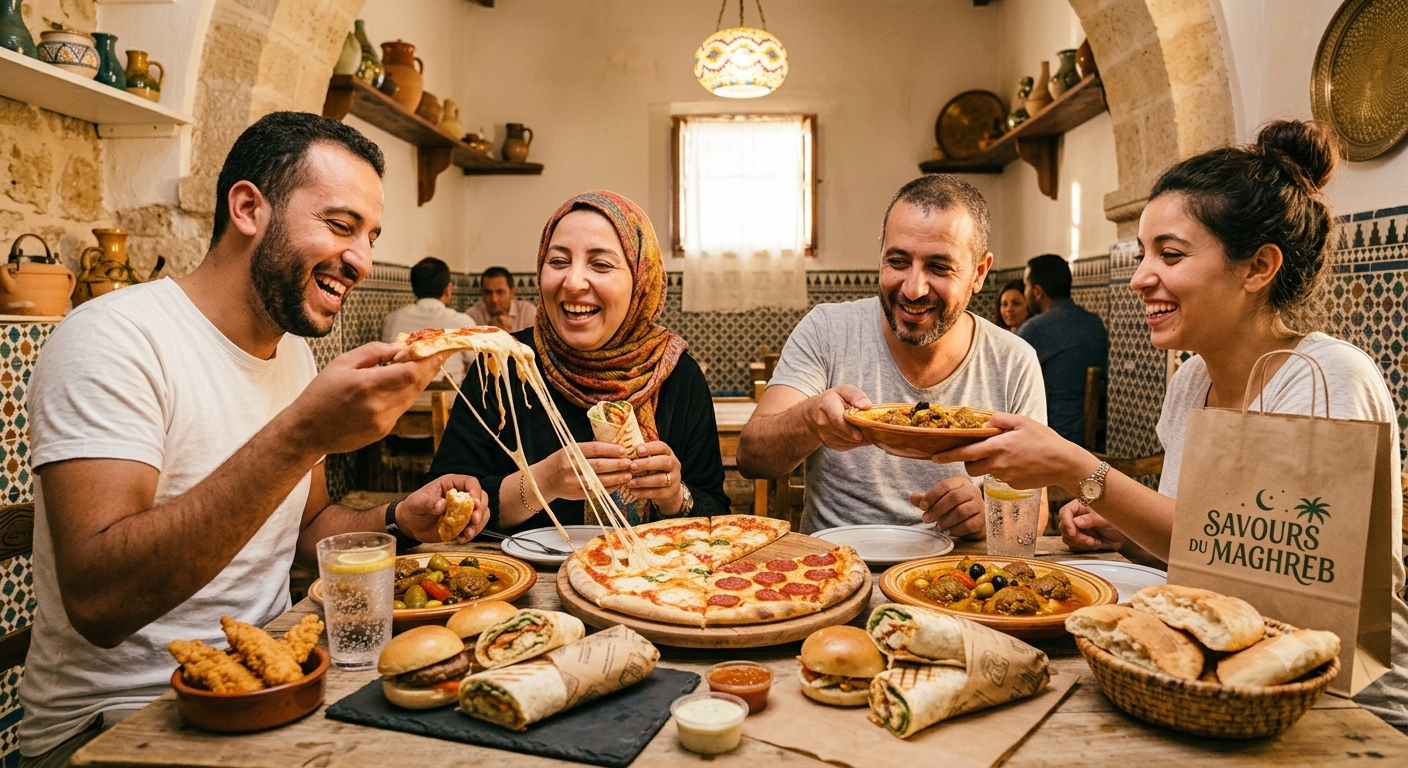
\includegraphics[width=0.55\textwidth,keepaspectratio]{image_repas.png}
    \caption{Illustration du service de commande de repas}
\end{figure}

Ce service correspond au cas d'usage le plus fréquent des applications de livraison, et c'est également celui qui a servi de base pour construire le reste du système~: le mécanisme de commande, de suivi et de dispatch décrit dans les chapitres suivants a d'abord été pensé pour ce service, avant d'être réutilisé pour les courses au supermarché.

\subsection{Achat de produits}

Sur le même principe, le client peut faire ses courses dans un supermarché partenaire directement depuis l'application, sans avoir à s'y déplacer.

\begin{figure}[H]
    \centering
    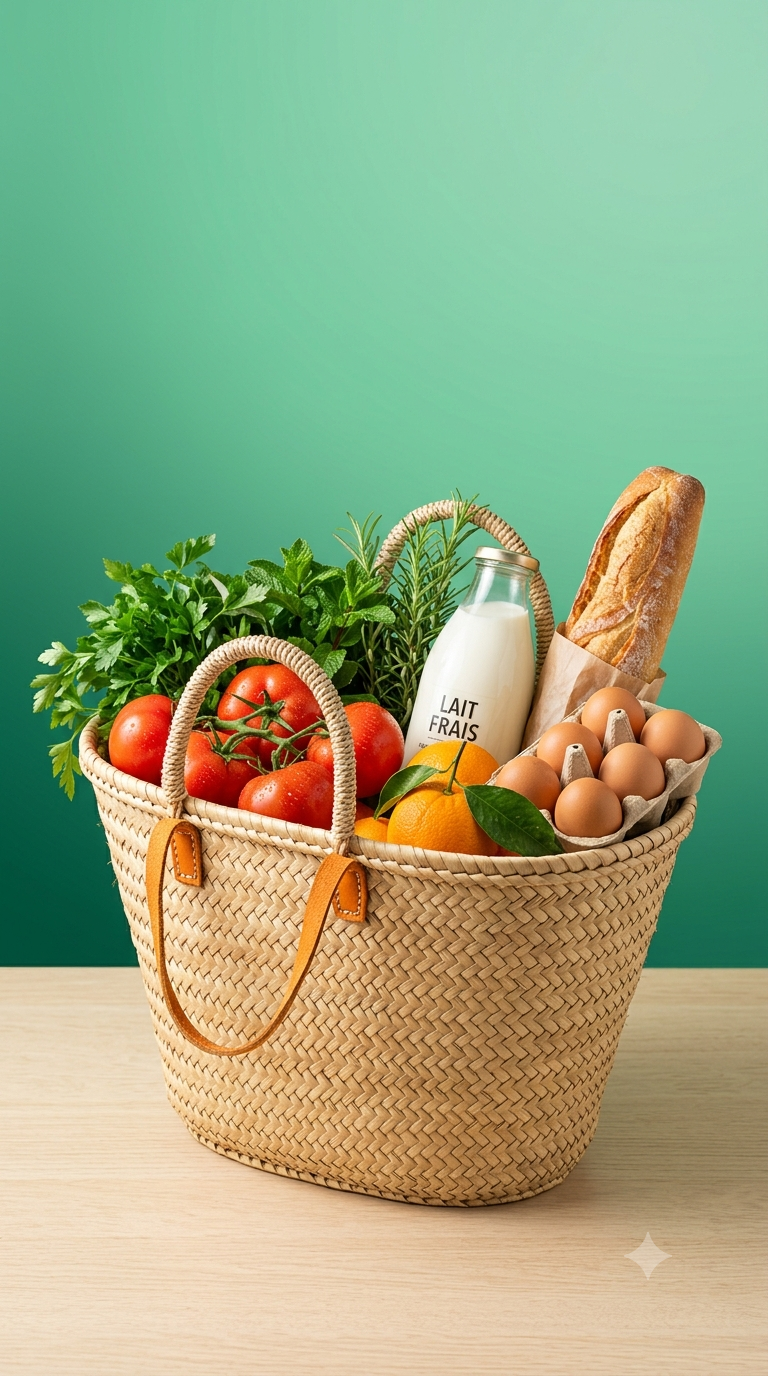
\includegraphics[width=0.55\textwidth,keepaspectratio]{image_supermarche.png}
    \caption{Illustration du service d'achat de produits}
\end{figure}

La différence technique avec la commande de repas est limitée~: un supermarché est traité comme un partenaire au même titre qu'un restaurant, et un produit de supermarché suit une gestion de stock légèrement différente de celle d'un plat préparé, comme expliqué au chapitre~2.

\subsection{Livraison de colis entre particuliers}

Ce service permet à un client d'envoyer un objet ou un colis directement à une autre personne, sans passer par un commerçant. Le client saisit l'adresse de récupération, l'adresse de dépôt, une description du colis, puis un livreur disponible prend en charge le transport.

\begin{figure}[H]
    \centering
    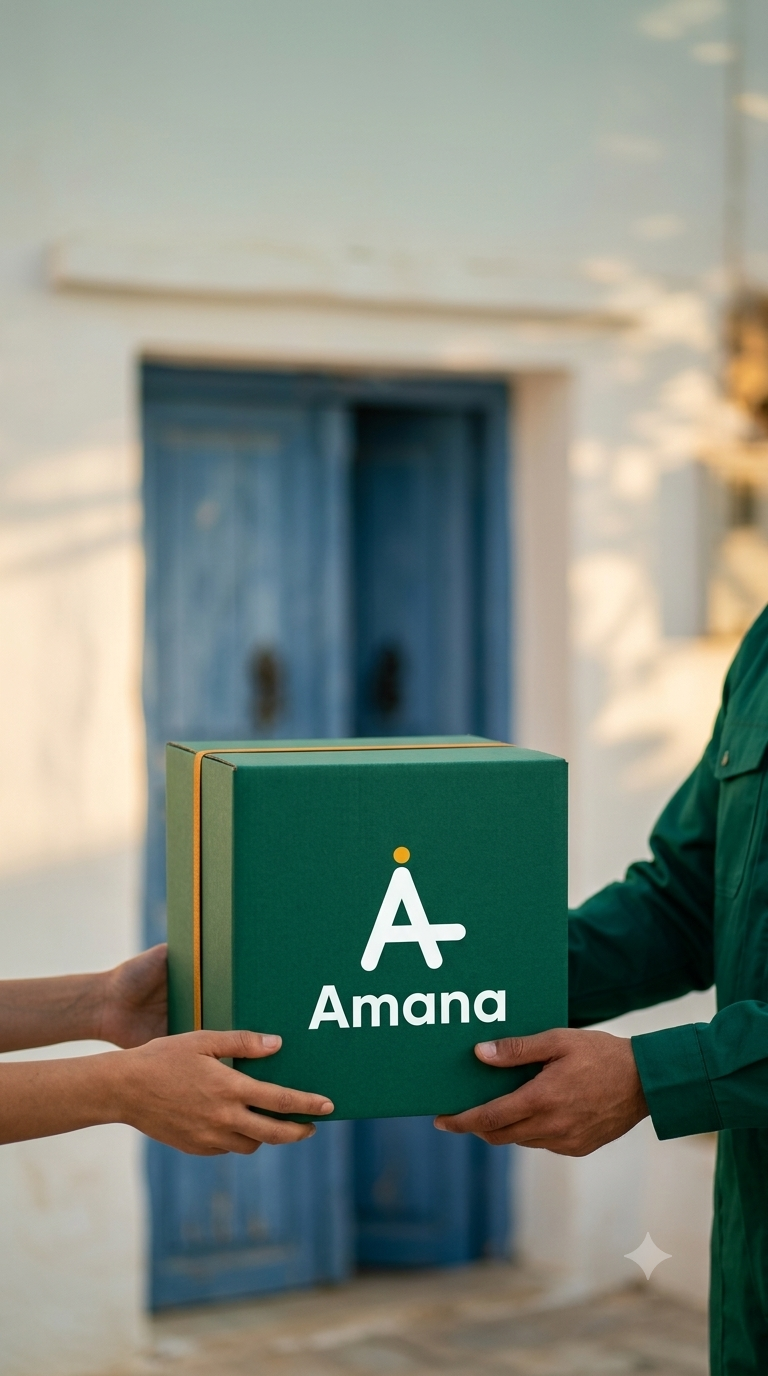
\includegraphics[width=0.5\textwidth,keepaspectratio]{colis.png}
    \caption{Illustration du service de livraison de colis entre particuliers (P2P)}
\end{figure}

C'est le service le plus proche d'un modèle de coursier à la demande. Il ne fait intervenir aucun partenaire commercial, ce qui simplifie son fonctionnement mais l'éloigne aussi du mécanisme habituel de préparation d'une commande, comme le montre le diagramme de séquence dédié présenté au chapitre~2.

\subsection{Paiement de factures}

Enfin, l'application permet à un client de faire payer une facture par un livreur, sans avoir à se déplacer jusqu'au guichet concerné.

\begin{figure}[H]
    \centering
    
\includegraphics[width=0.5\textwidth,keepaspectratio]{facture.png}
    \caption{Illustration du service de paiement de factures}
\end{figure}

Ce service répond à un besoin très concret dans le contexte tunisien, où le paiement de certaines factures nécessite encore un déplacement physique. Il complète l'offre d'Amana en dépassant le seul cadre de la livraison de produits.

\section{Analyse des solutions existantes}

L'analyse des solutions déjà présentes sur le marché est une étape nécessaire avant de concevoir une nouvelle plateforme. Elle permet de savoir ce qui existe déjà, ce qui fonctionne bien, et surtout ce qui manque. Face à la multitude d'applications de livraison, l'étude s'est concentrée sur les plateformes les plus actives en Tunisie, ainsi que sur une référence internationale.

\subsection{Panorama des applications de livraison}

Les applications de livraison peuvent être classées selon les services qu'elles proposent.

\vspace{0.3cm}
\noindent\textbf{Yassir Express} propose la livraison de repas préparés, de produits cosmétiques ainsi que de fruits et légumes.

\begin{figure}[H]
    \centering
    \fbox{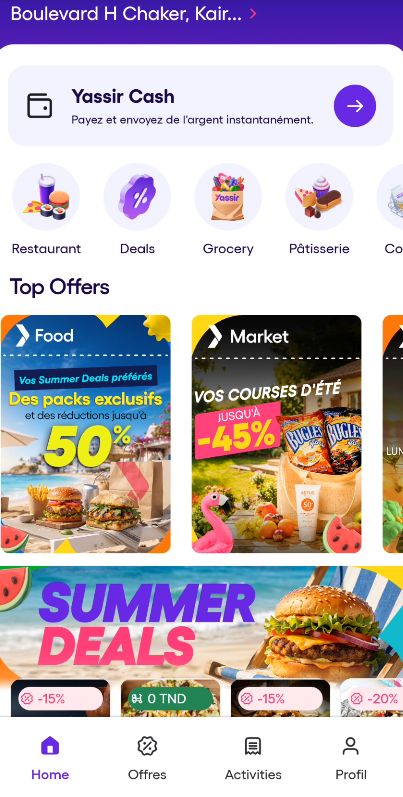
\includegraphics[width=0.85\textwidth,keepaspectratio]{yassir_interface_1.png}}
    \caption{Captures d'écran de l'application Yassir Express~\cite{yassir_site}}
\end{figure}

Les écrans ci-dessus montrent une interface classique de type liste de commerces puis fiche produit, proche de ce que propose Amana pour la commande de repas.

\begin{figure}[H]
    \centering
    \fbox{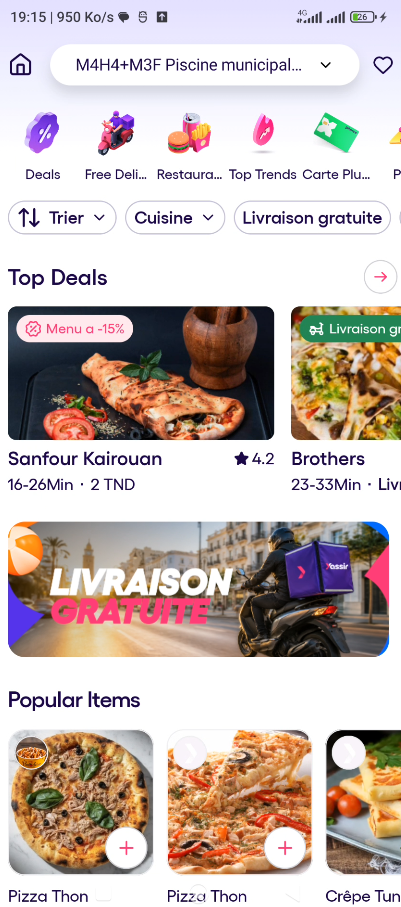
\includegraphics[width=0.85\textwidth,keepaspectratio]{yassir_interface_2.png}}
    \caption{Écran de suivi de commande de l'application Yassir Express~\cite{yassir_site}}
\end{figure}

L'écran de suivi confirme que la géolocalisation du livreur est un standard du secteur, qu'Amana reprend également.

\vspace{0.3cm}
\noindent\textbf{Livrina} regroupe la commande de repas, les achats du quotidien et le paiement de factures, avec un système d'envoi de colis entre particuliers.

\begin{figure}[H]
    \centering
    \fbox{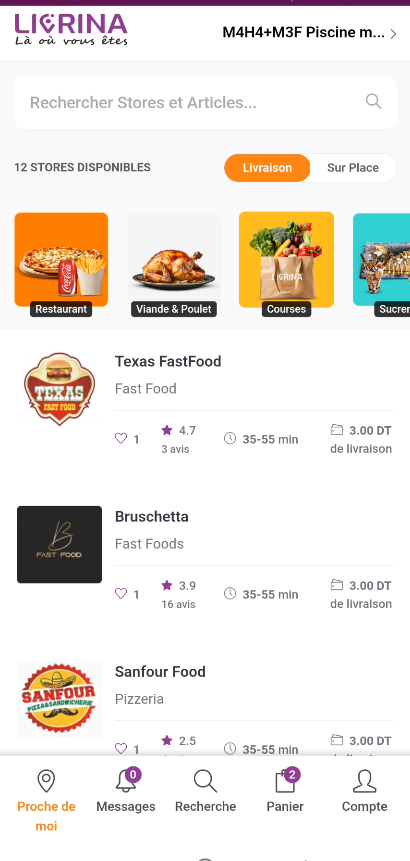
\includegraphics[width=0.85\textwidth,keepaspectratio]{livrina_interface.png}}
    \caption{Capture d'écran de l'application Livrina~\cite{livrina_site}}
\end{figure}

Livrina est, parmi les applications tunisiennes étudiées, celle dont le périmètre de services se rapproche le plus de celui d'Amana~: elle aussi combine repas, courses, factures et colis P2P dans une seule application.

\vspace{0.3cm}
\noindent\textbf{Glovo}, \textbf{KooL} et \textbf{ZigZag Delivery} complètent ce panorama. Glovo est une plateforme internationale multi-services permettant de commander des repas, de faire des achats du quotidien et d'expédier de petits colis en zone urbaine~\cite{glovo_site}. KooL est une application tunisienne dédiée à la livraison de repas à domicile, avec un suivi de commande en temps réel~\cite{kool_site}. ZigZag Delivery est une solution tunisienne spécialisée dans la commande et la livraison rapide de repas, avec un service actif dans plusieurs villes du pays~\cite{zigzag_site}.

\subsection{Analyse détaillée des acteurs du marché}

\subsubsection*{\Large \textbf{1. Glovo}}
\vspace{0.2cm}

\noindent \textbf{\underline{Points forts~:}}
Interface moderne et simple à utiliser, large gamme de catégories (repas, courses, pharmacie) et forte notoriété internationale.

\vspace{0.2cm}
\noindent \textbf{\underline{Limites~:}}
\begin{itemize}
    \item \textbf{Absence à Kairouan~:} le service cible surtout Tunis et les grandes villes côtières.
    \item \textbf{Commissions élevées~:} les taux prélevés aux commerçants partenaires, entre 20\,\% et 30\,\%, réduisent fortement leurs marges.
    \item \textbf{Rigidité~:} faible capacité à s'adapter aux besoins des villes secondaires.
\end{itemize}

\vspace{0.4cm}

\subsubsection*{\Large \textbf{2. Yassir Express}}
\vspace{0.2cm}

\noindent \textbf{\underline{Points forts~:}}
Écosystème régional qui combine transport et livraison, avec une bonne infrastructure technique.

\vspace{0.2cm}
\noindent \textbf{\underline{Limites~:}}
\begin{itemize}
    \item \textbf{Couverture instable à Kairouan~:} le service y est indisponible ou peu fiable.
    \item \textbf{Offre peu diversifiée~:} l'accent est mis sur la restauration rapide, sans réel service de coursier au quotidien.
    \item \textbf{Disponibilité irrégulière~:} nombre de livreurs insuffisant en dehors des grands axes urbains.
\end{itemize}

\vspace{0.4cm}

\subsubsection*{\Large \textbf{3. KooL}}
\vspace{0.2cm}

\noindent \textbf{\underline{Points forts~:}}
Application bien implantée dans le Grand Tunis et le Cap Bon pour la livraison de repas.

\vspace{0.2cm}
\noindent \textbf{\underline{Limites~:}}
\begin{itemize}
    \item \textbf{Absence à Kairouan~:} l'application n'y opère pas.
    \item \textbf{Spécialisation unique~:} service limité à la nourriture, sans envoi de colis ni gestion de courses.
    \item \textbf{Retards aux heures de pointe~:} difficultés fréquentes pendant les heures de repas.
\end{itemize}

\vspace{0.4cm}

\subsubsection*{\Large \textbf{4. ZigZag Delivery}}
\vspace{0.2cm}

\noindent \textbf{\underline{Points forts~:}}
Solution locale réactive pour la livraison rapide auprès de restaurants partenaires.

\vspace{0.2cm}
\noindent \textbf{\underline{Limites~:}}
\begin{itemize}
    \item \textbf{Absence à Kairouan~:} déploiement limité à quelques zones urbaines.
    \item \textbf{Fonctionnalités limitées~:} suivi en temps réel parfois manquant.
    \item \textbf{Peu de polyvalence~:} pas de services de proximité au-delà des repas.
\end{itemize}

\vspace{0.4cm}

\subsubsection*{\Large \textbf{5. Livrina}}
\vspace{0.2cm}

\noindent \textbf{\underline{Points forts~:}}
Plateforme tunisienne spécialisée dans la logistique du dernier kilomètre, avec un périmètre de services proche de celui d'Amana.

\vspace{0.2cm}
\noindent \textbf{\underline{Limites~:}}
\begin{itemize}
    \item \textbf{Absence à Kairouan~:} activité concentrée sur Tunis et le Sahel.
    \item \textbf{Modèle plus e-commerce~:} moins adapté à la livraison instantanée de repas.
\end{itemize}

\section{Limites des solutions existantes}

L'analyse détaillée ci-dessus fait ressortir quatre limites communes à l'ensemble des plateformes étudiées.

\begin{enumerate}
    \item \textbf{Une couverture géographique inégale~:} aucune des cinq plateformes étudiées n'est activement présente à Kairouan. Les habitants et les commerçants locaux ne disposent donc d'aucun service numérique de livraison fiable.
    \item \textbf{L'absence d'une offre multi-services complète~:} même Livrina, la plus proche d'Amana par ses services, ne couvre pas exactement le même périmètre. La plupart des autres applications obligent l'utilisateur à cumuler plusieurs applications différentes pour commander un repas, envoyer un colis ou payer une facture.
    \item \textbf{Des commissions parfois lourdes pour le commerce local~:} le cas de Glovo, avec des taux pouvant atteindre 30\,\%, montre que ces commissions peuvent décourager les petits commerçants indépendants.
    \item \textbf{Une logistique pensée pour les grandes villes~:} les outils de géolocalisation génériques utilisés par ces plateformes ne sont pas toujours adaptés aux quartiers anciens ou aux zones moins densément cartographiées.
\end{enumerate}

Le tableau~\ref{tab:comparatif_existant} résume cette comparaison selon plusieurs critères.

\begin{table}[h!]
\centering
\scriptsize
\setlength{\tabcolsep}{3pt}
\renewcommand{\arraystretch}{1.25}
\begin{tabular}{|l|c|c|c|c|c|}
\hline
\textbf{Critère} & \textbf{Glovo} & \textbf{Yassir Express} & \textbf{KooL} & \textbf{ZigZag Delivery} & \textbf{Livrina} \\ \hline
Livraison de repas & Oui & Oui & Oui & Oui & Non \\ \hline
Livraison P2P (colis) & Partiel & Non & Non & Non & Non \\ \hline
Couverture de Kairouan & \textbf{Non} & \textbf{Non / Instable} & \textbf{Non} & \textbf{Non} & \textbf{Non} \\ \hline
Paiement de factures & Non & Non & Non & Non & Non \\ \hline
Adaptation au commerce local & Faible & Moyenne & Faible & Faible & Moyenne \\ \hline
Paiement à la livraison (cash) & Oui & Oui & Oui & Oui & Oui \\ \hline
Suivi en temps réel & Oui & Oui & Moyen & Faible & Moyen \\ \hline
\end{tabular}
\caption{Analyse comparative des fonctionnalités des plateformes existantes}
\label{tab:comparatif_existant}
\end{table}

Ce tableau montre qu'aucune des plateformes étudiées ne réunit à la fois la couverture de Kairouan, l'offre multi-services et le paiement de factures. C'est précisément l'espace laissé libre par le marché actuel, et c'est sur cet espace que se positionne le projet Amana.

\section{Solution proposée}

Pour répondre aux limites identifiées, ce projet propose le développement d'une plateforme mobile et web multiservices, pensée dès le départ pour Kairouan plutôt que comme une extension tardive d'un service déjà pensé pour Tunis. Plutôt que de se limiter à la restauration, Amana adopte une approche généraliste~: le client peut commander dans un restaurant, faire ses courses dans un supermarché, envoyer un colis à un proche ou faire payer une facture, le tout depuis la même application.

L'innovation d'Amana ne tient donc pas à une technologie inédite, mais à la combinaison de services qui, ailleurs, sont proposés séparément. Le règlement de factures via l'application fait gagner du temps aux utilisateurs, et le service de livraison entre particuliers (P2P) permet l'envoi sécurisé d'objets personnels grâce au réseau de livreurs déjà mobilisé pour les commandes classiques.

D'un point de vue stratégique, une phase pilote est d'abord lancée à Kairouan pour valider le modèle, avant d'envisager une extension progressive à d'autres gouvernorats. En connectant clients, commerçants et livreurs autour d'un même système, Amana ne se limite pas à optimiser la logistique~: elle propose une expérience utilisateur moderne, adaptée aux habitudes économiques locales.

\section{Cahier des charges}

Le cahier des charges définit de façon précise les objectifs du système et les fonctionnalités attendues. Il sert de référence pour les phases de conception et de développement présentées dans les chapitres suivants.

L'objectif principal est de concevoir une plateforme capable de fournir les quatre services décrits plus haut de manière simple et fiable. Le client doit pouvoir commander un produit ou un plat proposé par un restaurant, une boutique ou un supermarché, tout en bénéficiant d'un service de livraison organisé. Il doit également pouvoir régler certaines factures directement depuis l'application, et envoyer un colis à une autre personne en utilisant les livreurs disponibles sur la plateforme.

Le système repose sur l'interaction de quatre acteurs principaux~: le client, qui utilise l'application pour commander, payer des factures ou envoyer des colis~; le commerçant, qui propose ses produits et gère les commandes reçues~; le livreur, qui assure le transport~; et l'administrateur, qui supervise le fonctionnement de la plateforme et gère les utilisateurs.

\section{Identification des acteurs}

\subsection{Le Client}
Le client est l'utilisateur principal de l'application. Il consulte les produits ou les plats disponibles, passe des commandes, paie certaines factures et envoie des colis à d'autres personnes grâce au service de livraison entre particuliers. Il peut à tout moment suivre l'état de ses commandes et de ses livraisons depuis l'application.

\subsection{Le Commerçant}
Le commerçant regroupe les différents vendeurs présents sur la plateforme~: restaurants, boutiques ou supermarchés. Il propose ses produits ou ses plats, gère les informations de son catalogue, reçoit les commandes des clients, les prépare et les met à disposition pour la livraison.

\subsection{Le Livreur}
Le livreur assure le transport des commandes et des colis entre les différents utilisateurs du système. Il reçoit les missions attribuées par la plateforme, récupère les produits auprès des commerçants ou des expéditeurs, puis les livre aux destinataires dans les délais prévus.

\subsection{L'Administrateur}
L'administrateur supervise le fonctionnement global de l'application. Il gère les comptes utilisateurs, suit les activités réalisées sur la plateforme, et intervient en cas de problème technique pour maintenir la qualité du service.

\section{Besoins fonctionnels}

Les besoins fonctionnels décrivent les actions que chaque acteur doit pouvoir réaliser à travers la plateforme.

\subsection{Besoins fonctionnels du client}

\textbf{Gestion du compte~:} créer un profil sécurisé et accéder au catalogue de services après authentification.

\vspace{0.3cm}
\textbf{Achat et commande~:} parcourir les menus des restaurants ou les rayons des supermarchés partenaires, filtrer par catégorie, consulter le détail des articles et valider un panier.

\vspace{0.3cm}
\textbf{Suivi en temps réel~:} suivre la progression de sa commande, de la préparation par le commerçant jusqu'à la réception, avec la position du livreur affichée sur une carte.

\vspace{0.3cm}
\textbf{Paiement de factures~:} régler une facture directement depuis l'application, sans passer par un guichet.

\vspace{0.3cm}
\textbf{Livraison entre particuliers~:} demander un coursier pour transporter un colis, en indiquant le point de collecte, la destination et les caractéristiques de l'objet.

\vspace{0.3cm}
\textbf{Historique~:} consulter à tout moment les commandes passées, les factures réglées et les colis envoyés.

\subsection{Besoins fonctionnels du commerçant}
Le commerçant doit pouvoir créer un compte professionnel donnant accès à un espace dédié à la gestion de ses produits. Il ajoute, modifie ou supprime des articles de son catalogue, met à jour les prix, les descriptions et la disponibilité. Il reçoit les commandes des clients, consulte leur détail pour les préparer, confirme leur disponibilité pour la livraison, et suit l'historique de ses ventes.

\subsection{Besoins fonctionnels du livreur}
Le livreur crée un compte et accède à son espace personnel après authentification. Il consulte les missions qui lui sont proposées, les accepte ou les refuse selon sa disponibilité. Une fois une mission acceptée, il récupère la commande puis la livre à l'adresse indiquée, en mettant à jour le statut de la livraison à chaque étape (récupérée, en cours de livraison, livrée).

\subsection{Besoins fonctionnels de l'administrateur}
L'administrateur gère les comptes des clients, des commerçants et des livreurs~: il vérifie les informations fournies à l'inscription, active ou désactive des comptes si nécessaire. Il surveille l'activité de la plateforme pour garantir la qualité du service, et intervient en cas de litige ou de problème technique.

\section{Besoins non fonctionnels}

Les besoins non fonctionnels concernent la qualité globale du système plutôt que les actions précises des utilisateurs~: performance, sécurité, disponibilité et fiabilité.

\subsection{Besoins non fonctionnels du client}
L'application doit rester simple et rapide à prendre en main, avec un temps de réponse court lors du chargement des pages ou de la validation d'une commande. Les données personnelles et les informations de paiement doivent être protégées contre tout accès non autorisé, et le service doit rester disponible en permanence.

\subsection{Besoins non fonctionnels du commerçant}
L'interface doit rester simple à utiliser sans compétence technique particulière. Le système doit traiter les commandes en temps réel, en particulier lors des périodes de forte activité, et garantir l'intégrité des données commerciales.

\subsection{Besoins non fonctionnels du livreur}
L'application doit être rapide à consulter en situation de mobilité, avec des notifications reçues en temps réel pour les nouvelles missions. La précision de la géolocalisation est essentielle pour optimiser les trajets.

\subsection{Besoins non fonctionnels de l'administrateur}
L'accès aux fonctionnalités d'administration doit être protégé, avec un contrôle strict des permissions. Le système doit rester performant même avec un grand nombre d'utilisateurs et d'opérations simultanées, et doit pouvoir évoluer facilement pour accueillir de nouvelles fonctionnalités.

\section{Contraintes du projet}

Sur le plan technique, l'application doit être développée avec des outils adaptés au développement mobile multiplateforme, tout en garantissant de bonnes performances. Le système doit intégrer plusieurs services distincts au sein d'une seule plateforme, ce qui complexifie la conception et impose une organisation rigoureuse.

Sur le plan organisationnel, le projet devait être réalisé dans un temps limité, ce qui a exigé une planification par itérations plutôt qu'une planification figée dès le départ. S'agissant d'un projet académique, le travail devait suivre une méthodologie claire, présentée à la section suivante.

Sur le plan de l'utilisation, l'application doit rester simple malgré la diversité des fonctionnalités proposées. Enfin, la sécurité constitue une contrainte transversale~: protection des données personnelles, fiabilité des paiements, et disponibilité continue du service.

\section{Méthodologie de travail}

\subsection{Identification de la méthodologie}

La réalisation de la plateforme Amana s'est appuyée sur une approche de développement itératif et agile. Plutôt que de tout planifier en amont comme le préconise le modèle en cascade, le travail a été structuré en cycles successifs, chacun aboutissant à une fonctionnalité opérationnelle et vérifiable. Ce choix a permis d'ajuster progressivement les orientations techniques en fonction des difficultés rencontrées à chaque étape.

\subsection{Définition}

Le développement itératif désigne une démarche où le produit prend forme par enrichissements successifs. À chaque cycle, on traverse les étapes de modélisation, réalisation, vérification et mise en service partielle. Cette façon de travailler rejoint les valeurs du Manifeste Agile~\cite{agile_manifesto}, qui place la capacité d'adaptation et la livraison régulière de résultats concrets au-dessus d'une planification figée à l'avance.

\subsection{Avantages}

Le recours à cette méthode a apporté plusieurs bénéfices tout au long du projet~:

\begin{itemize}
    \item \textbf{Identification rapide des anomalies~:} en testant chaque fonctionnalité dès sa réalisation, les problèmes techniques sont repérés avant de se propager.
    \item \textbf{Capacité d'adaptation~:} un besoin qui évolue en cours de développement peut être intégré à l'itération suivante sans remettre en cause le travail déjà fait.
    \item \textbf{Progression vérifiable~:} chaque itération produit un résultat testable, ce qui permet de mesurer concrètement l'avancement.
    \item \textbf{Adéquation avec un marché incertain~:} pour un projet lancé sur un marché encore en construction, comme celui de la livraison à Kairouan, cette souplesse est particulièrement utile.
\end{itemize}

\subsection{Application concrète dans le projet}

Cette manière de travailler s'est traduite de façon visible à plusieurs moments du développement~:

\begin{itemize}
    \item \textbf{Construction couche par couche~:} chaque fonctionnalité a suivi le même enchaînement, de la base de données vers la logique serveur, puis vers l'interface mobile. La mise en place du programme de fidélité, par exemple, a commencé par la création des tables nécessaires, avant l'interface de suivi puis les effets visuels.
    \item \textbf{Résolution des anomalies au fil de l'eau~:} certains défauts ne sont apparus que lors des essais sur un appareil physique. C'est le cas d'un problème d'ordre d'affichage des options de personnalisation d'un plat, causé par un comportement implicite de la bibliothèque PostgREST, diagnostiqué puis corrigé sans interrompre le reste du projet.
    \item \textbf{Ajustement des spécifications~:} le nombre de statuts possibles pour une commande est passé de cinq à huit au fil du temps, afin de mieux représenter les situations réelles rencontrées, notamment avec l'introduction des états \textit{preparing} et \textit{onTheWay}.
    \item \textbf{Suivi documentaire régulier~:} un fichier de référence technique a été tenu à jour après chaque session de travail, pour garder une trace claire de l'avancement et faciliter la reprise du développement.
\end{itemize}

\begin{table}[H]
\centering
\begin{tabular}{|l|l|l|}
\hline
\textbf{Itération} & \textbf{Période} & \textbf{Fonctionnalités} \\
\hline
1 & Mai 2026 & Authentification, base de données, architecture \\
2 & Juin 2026 & Commandes, dispatch, suivi en temps réel \\
3 & Juillet 2026 & Fidélité, personnalisation du menu \\
4 & Août 2026 & Tests, corrections, préparation du déploiement \\
\hline
\end{tabular}
\caption{Planning des itérations du projet}
\end{table}

\section{Conclusion}

Ce premier chapitre a présenté le cadre général du projet~: le contexte qui justifie le choix de Kairouan, les quatre services proposés par Amana, l'analyse des solutions déjà présentes sur le marché tunisien, et les limites qui en ressortent. Cette analyse a conduit à la solution proposée et au cahier des charges, qui définit les acteurs du système ainsi que les besoins fonctionnels et non fonctionnels à satisfaire. La méthodologie de travail retenue, itérative et agile, a permis d'avancer par cycles courts tout en s'adaptant aux difficultés rencontrées. L'ensemble de ces éléments constitue la base sur laquelle s'appuie le chapitre suivant, consacré à l'analyse et à la conception du système.

%************CHAP2***********
\chapter{Analyse et conception du système}

\section{Introduction}

Le chapitre précédent a présenté les besoins du système et les quatre acteurs qui interagissent avec la plateforme Amana. Ce deuxième chapitre passe à une étape plus technique~: comprendre comment le système est structuré et comment il se comporte, avant de commencer à écrire du code. Le langage de modélisation UML~\cite{omg_uml} est utilisé pour représenter les fonctionnalités, l'architecture générale et les échanges entre les composants de l'application.

Le chapitre commence par identifier les principales fonctionnalités du système, avant de les représenter à travers un diagramme de cas d'utilisation puis une description détaillée de six scénarios clés. Il présente ensuite l'architecture générale de la plateforme, la modélisation des données à travers le diagramme de classes, et enfin le comportement dynamique du système à travers des diagrammes de séquence.

\section{Identification des fonctionnalités principales}

En reprenant les besoins fonctionnels définis au chapitre précédent, on peut regrouper les fonctionnalités de la plateforme Amana en cinq grandes familles~:

\begin{itemize}
    \item \textbf{Authentification et gestion de compte~:} inscription, connexion classique ou via Google, gestion du profil, pour les quatre types d'acteurs.
    \item \textbf{Commande et catalogue~:} consultation des restaurants et supermarchés, gestion du panier, validation d'une commande, gestion du catalogue côté commerçant.
    \item \textbf{Livraison~:} attribution d'une commande à un livreur, suivi en temps réel, mise à jour du statut jusqu'à la remise finale.
    \item \textbf{Services complémentaires~:} envoi de colis entre particuliers, paiement de factures, assistant conversationnel et recherche intelligente.
    \item \textbf{Gestion financière~:} portefeuille électronique, commissions, programme de fidélité, supervision par l'administrateur.
\end{itemize}

Ces cinq familles servent de fil conducteur pour les diagrammes présentés dans la suite de ce chapitre.

\section{Diagramme général des cas d'utilisation}

Le diagramme de cas d'utilisation représente, de manière simple, les fonctionnalités offertes par le système et les acteurs qui les déclenchent. Il met en évidence les interactions entre les acteurs externes — le client, le commerçant, le livreur et l'administrateur — et l'application, sans entrer dans le détail du fonctionnement interne. Vu le nombre de fonctionnalités couvertes par la plateforme, le diagramme a été réparti en quatre vues, une par acteur principal.

\begin{figure}[H]
    \centering
    \fbox{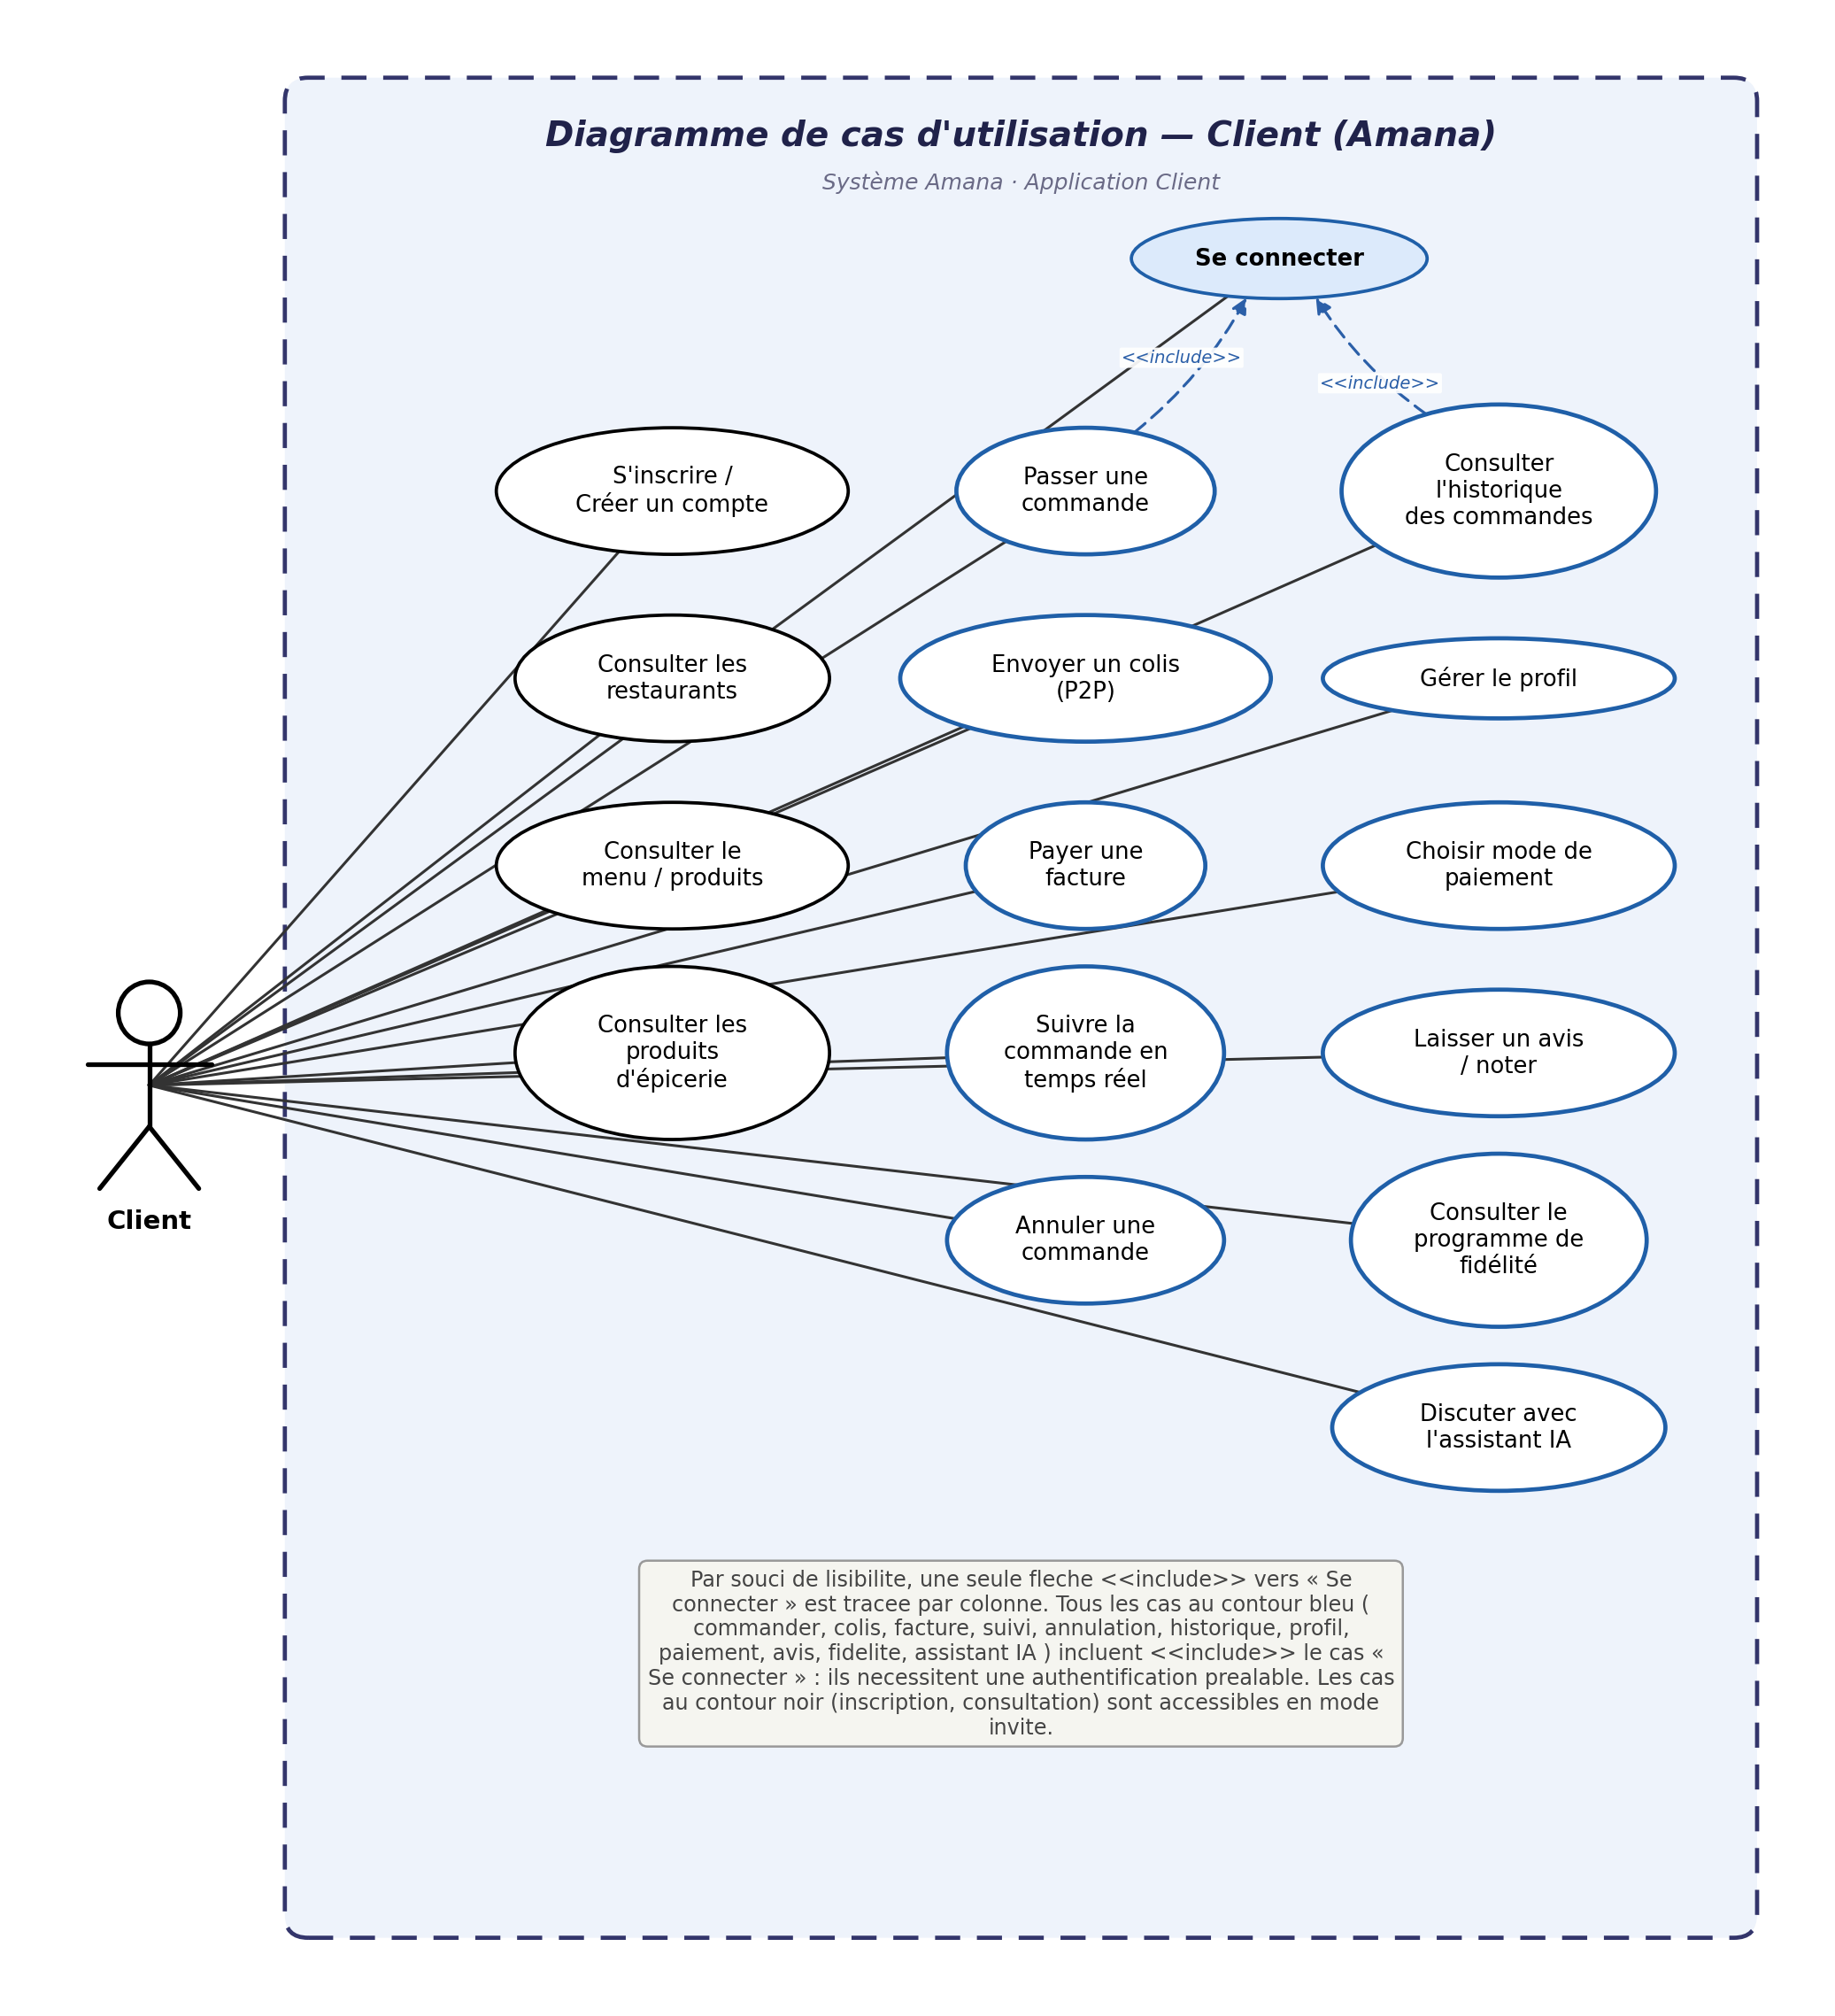
\includegraphics[width=\textwidth,height=0.85\textheight,keepaspectratio]{cas_utilisation_client_v2.png}}
    \caption{Diagramme de cas d'utilisation — acteur Client}
\end{figure}
\newpage

\begin{figure}[H]
    \centering
    \fbox{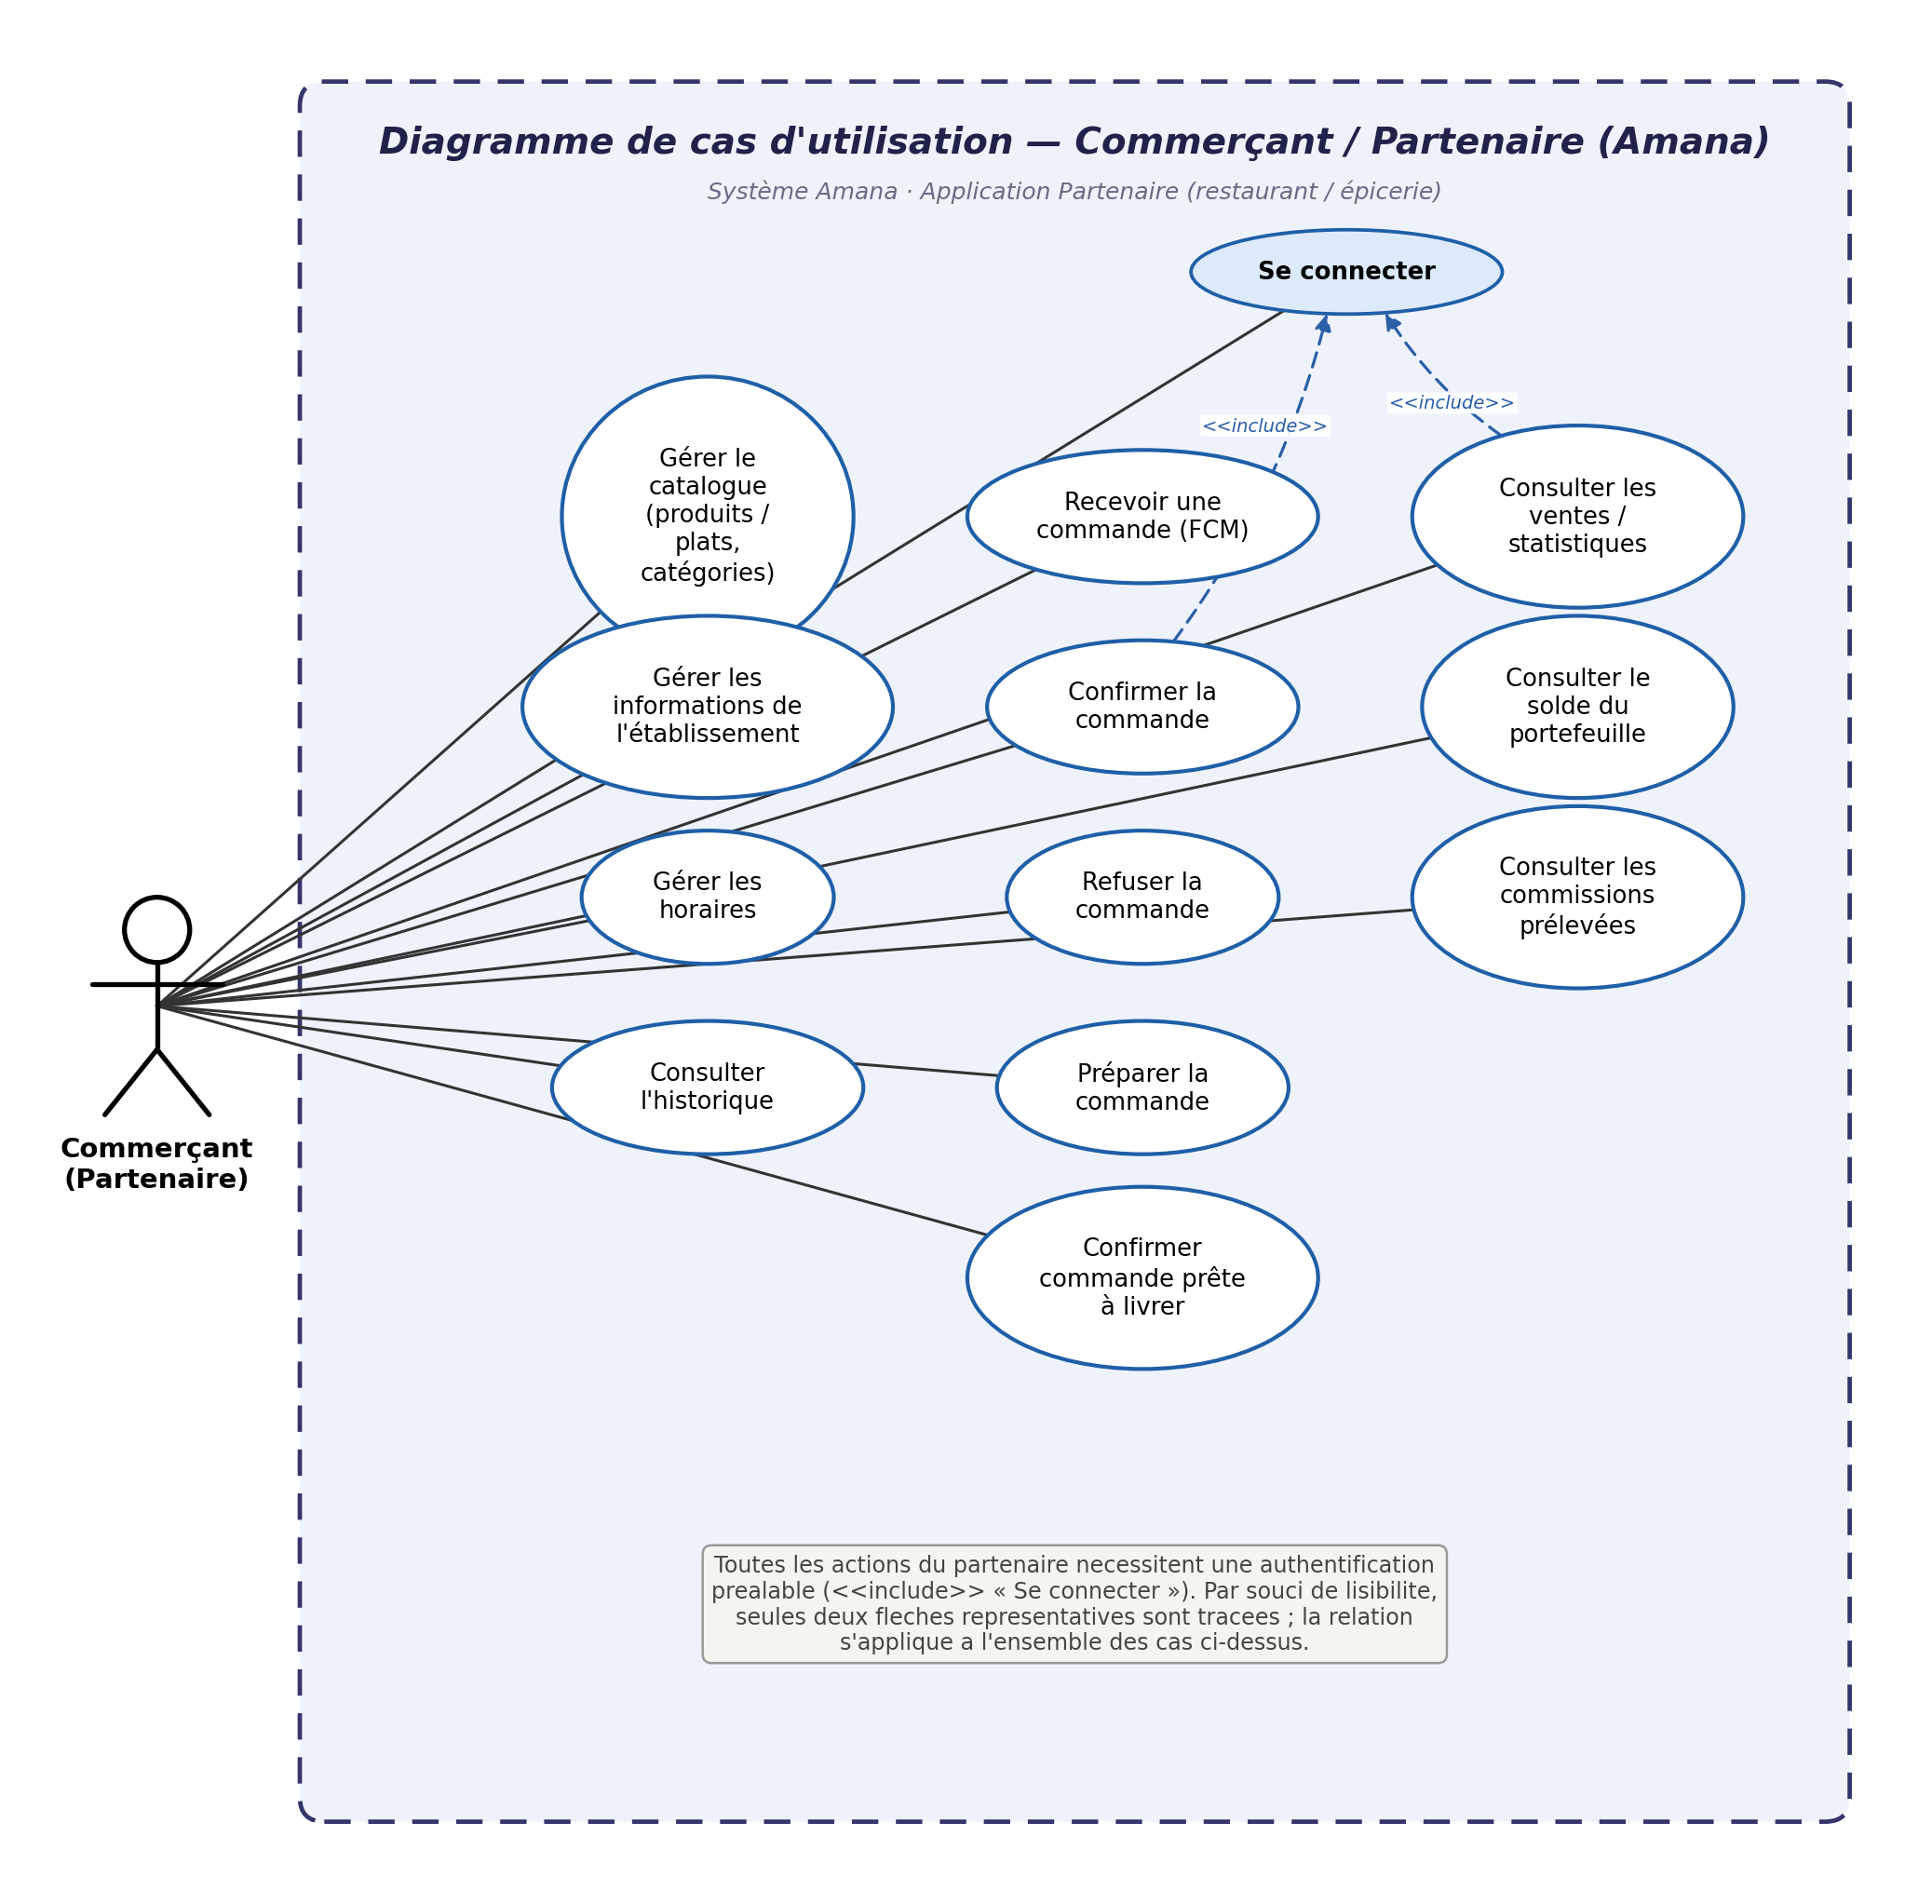
\includegraphics[width=\textwidth,height=0.85\textheight,keepaspectratio]{cas_utilisation_partenaire_v2.png}}
    \caption{Diagramme de cas d'utilisation — acteur Commerçant}
\end{figure}
\newpage

\begin{figure}[H]
    \centering
    \fbox{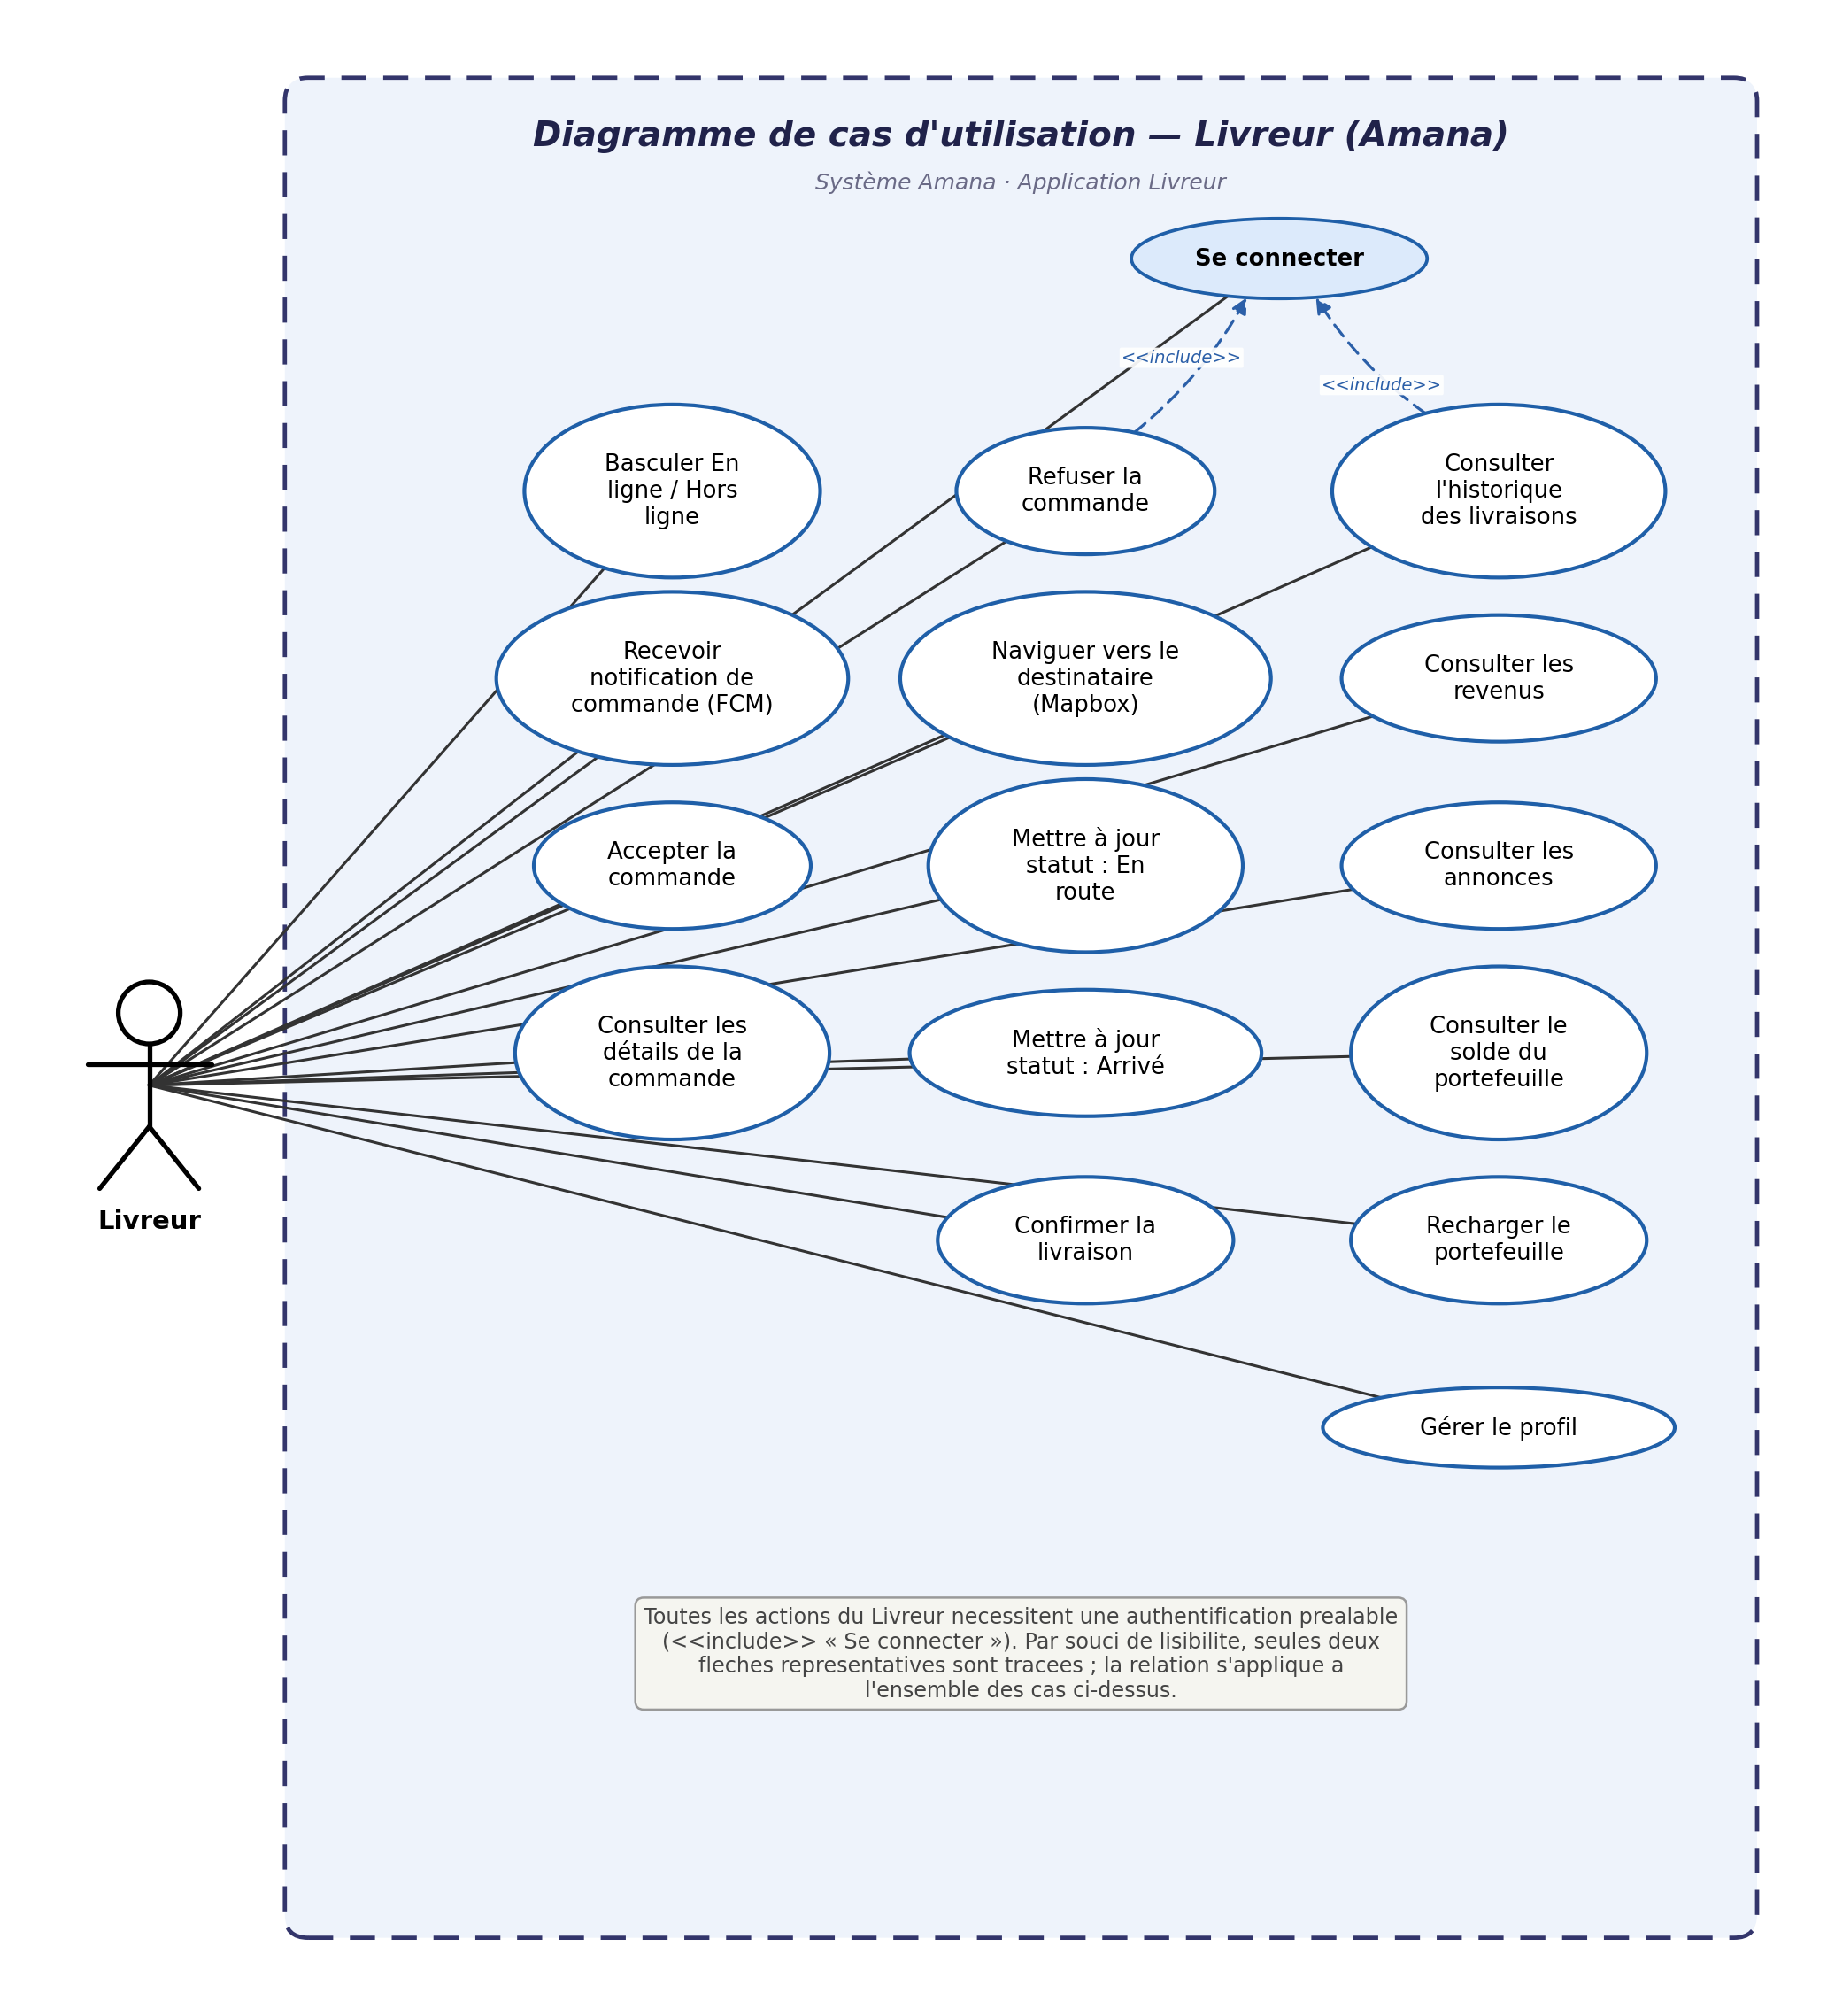
\includegraphics[width=\textwidth,height=0.85\textheight,keepaspectratio]{cas_utilisation_livreur_v2.png}}
    \caption{Diagramme de cas d'utilisation — acteur Livreur}
\end{figure}
\newpage

\begin{figure}[H]
    \centering
    \fbox{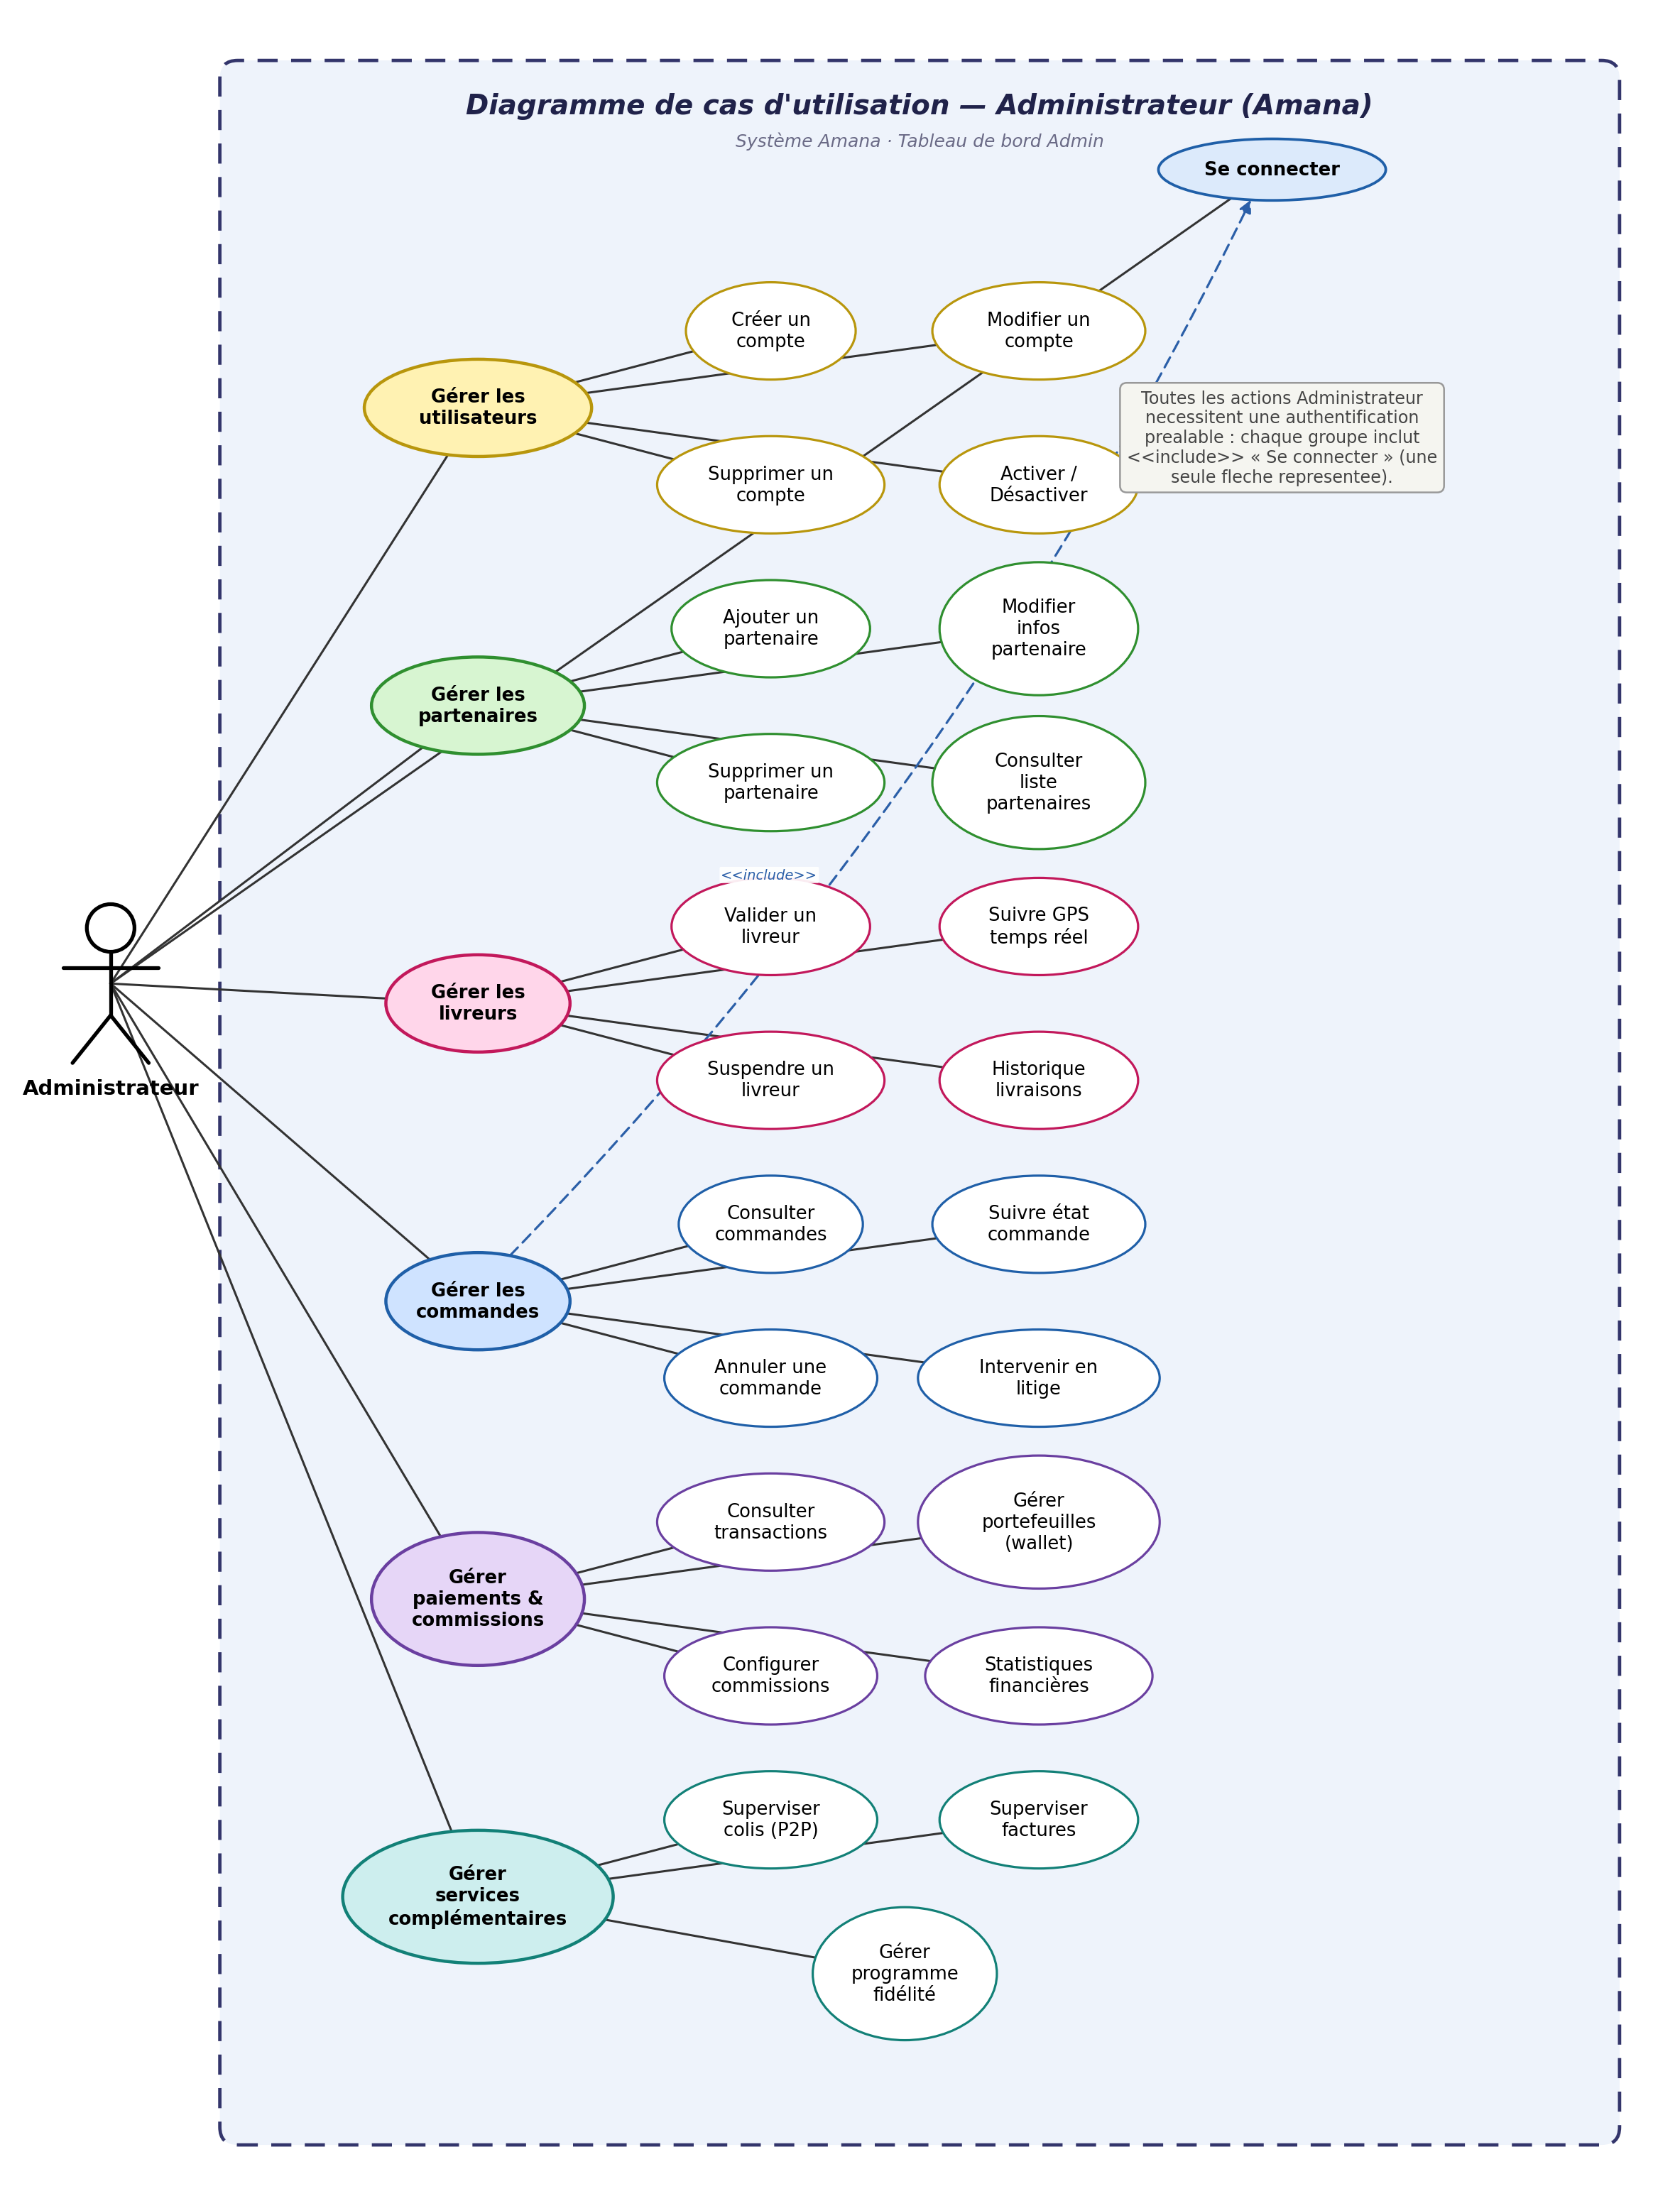
\includegraphics[width=\textwidth,height=0.85\textheight,keepaspectratio]{cas_utilisation_admin_v2.png}}
    \caption{Diagramme de cas d'utilisation — acteur Administrateur}
\end{figure}
\newpage

L'analyse de ces quatre vues montre une séparation claire des responsabilités. Le client est le moteur de l'activité~: c'est lui qui déclenche une commande ou une demande de livraison P2P. Le commerçant et le livreur agissent comme des exécutants opérationnels, chacun sur sa partie du processus. L'administrateur, de son côté, ne déclenche pas directement l'activité commerciale~: il conserve une vue transversale sur l'ensemble des échanges, pour garantir leur bon déroulement.

\section{Description des cas d'utilisation}

Six scénarios ont été choisis pour une description plus détaillée, car ils concentrent la plus grande partie de la logique du système~: l'authentification, la passation d'une commande, son suivi, sa livraison, l'ajout d'un plat du jour, et l'envoi d'un colis. Quatre d'entre eux ont fait l'objet d'un raffinement graphique, présenté ci-dessous sous forme de diagramme et de tableau descriptif~; les deux autres sont décrits textuellement, leur comportement dynamique étant détaillé plus loin dans les diagrammes de séquence de la section~\ref{sec:sequences}.

\subsection{Authentification et inscription}

Ce cas d'utilisation regroupe les différentes façons dont un utilisateur accède à l'application~: créer un nouveau compte avec un e-mail et un mot de passe, se connecter avec un compte existant, ou se connecter directement via un compte Google. Dans les trois cas, une vérification est faite juste après la connexion pour s'assurer qu'un numéro de téléphone est bien associé au profil~; si ce n'est pas le cas, l'utilisateur doit le renseigner avant de continuer. Ce cas d'utilisation est commun aux quatre applications de la plateforme, avec une seule différence~: l'application Administrateur ne propose pas d'inscription, seulement une connexion réservée aux comptes déjà autorisés.

\begin{table}[H]
\centering
\renewcommand{\arraystretch}{1.4}
\begin{tabular}{|l|l|p{7cm}|}
\hline
\textbf{Cas d'utilisation} & \textbf{Type} & \textbf{Description} \\
\hline
S'authentifier & Cas principal &
L'utilisateur accède à son compte pour utiliser l'application. \\
\hline
Créer un compte & Extension &
L'utilisateur saisit son nom, son e-mail et un mot de passe pour créer un nouveau profil. \\
\hline
Se connecter via Google & Extension &
L'utilisateur ouvre une session sans saisir de mot de passe, via son compte Google. \\
\hline
Renseigner le numéro de téléphone & Inclusion &
Si aucun numéro n'est encore associé au profil, l'utilisateur doit le saisir avant de continuer. \\
\hline
\end{tabular}
\caption{Description textuelle du cas d'utilisation~: Authentification et inscription}
\end{table}

\subsection{Passation d'une commande}

\begin{figure}[H]
    \centering
    \fbox{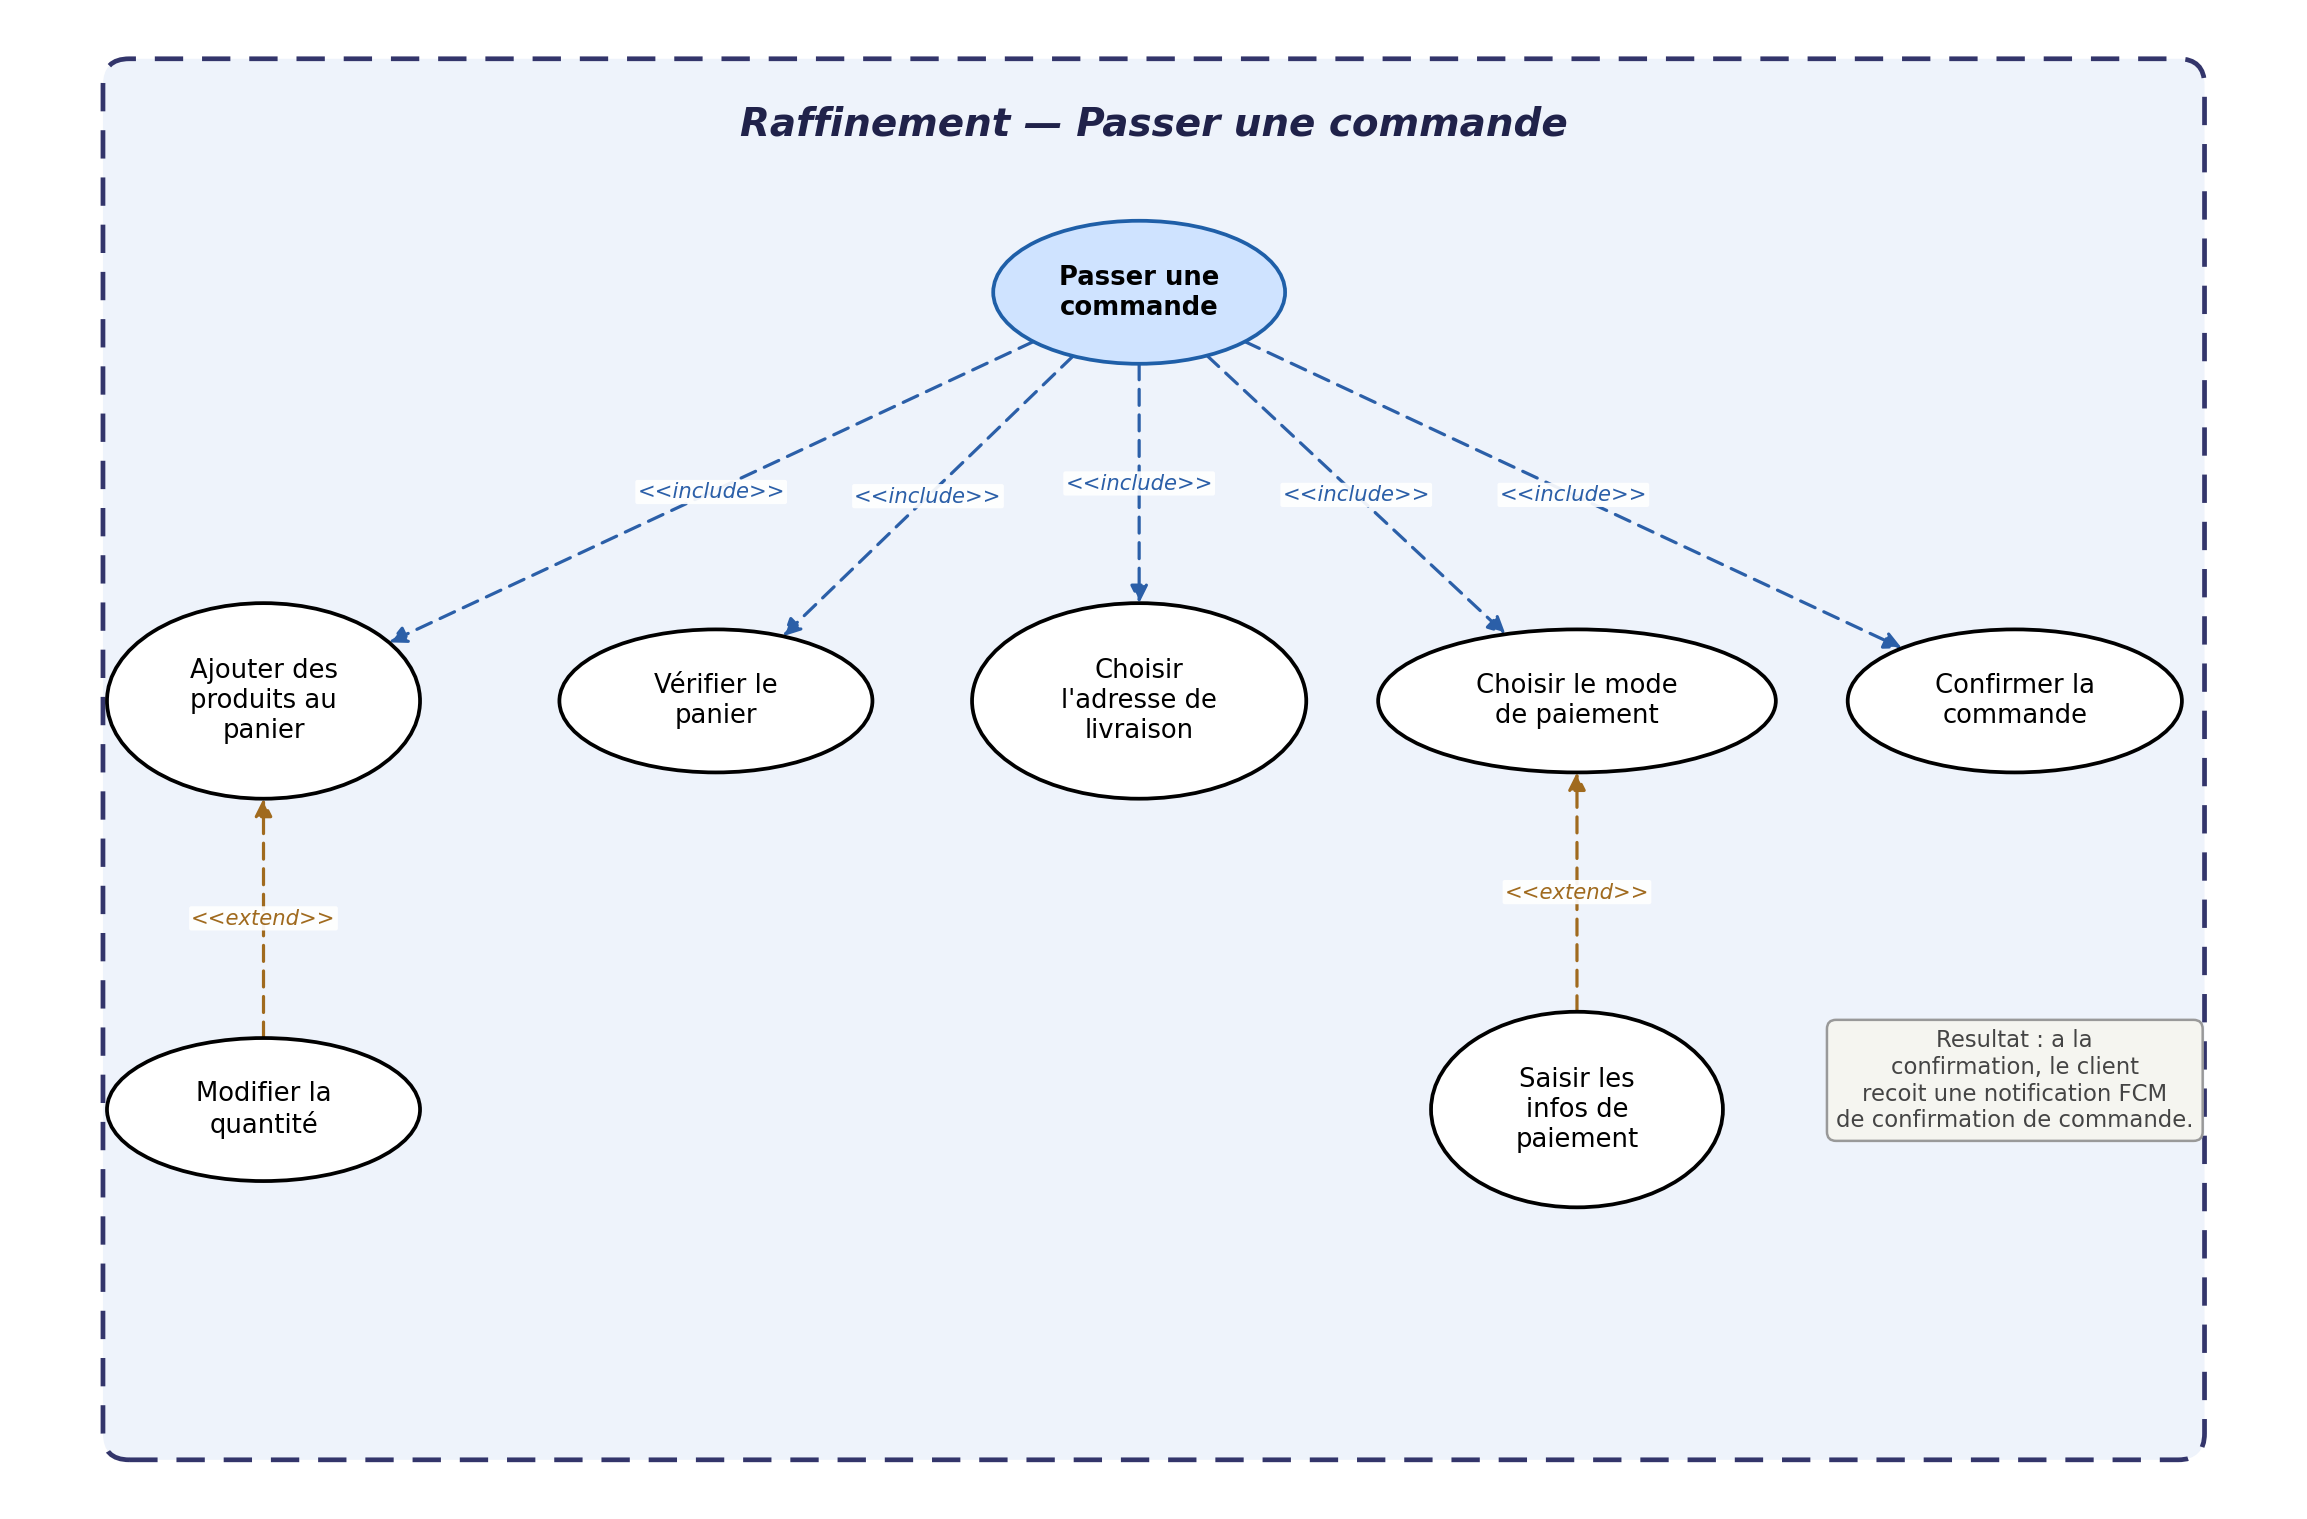
\includegraphics[width=\textwidth,height=0.6\textheight,keepaspectratio]{raffinement_passer_commande_v2.png}}
    \caption{Raffinement du cas d'utilisation~: passer une commande}
\end{figure}

Ce raffinement détaille les étapes que suit un client entre le choix des articles et la validation finale de sa commande.

\begin{table}[H]
\centering
\renewcommand{\arraystretch}{1.4}
\begin{tabular}{|l|l|p{7cm}|}
\hline
\textbf{Cas d'utilisation} & \textbf{Type} & \textbf{Description} \\
\hline
Passer une commande & Cas principal &
Le client réalise l'ensemble des étapes nécessaires pour soumettre sa commande, depuis la sélection des articles jusqu'à la validation finale. \\
\hline
Ajouter des produits au panier & Inclusion &
Le client sélectionne les articles souhaités, avec la possibilité de personnaliser chaque plat selon les options disponibles. \\
\hline
Modifier la quantité & Extension &
Depuis le panier, le client augmente ou réduit le nombre d'unités de chaque article. \\
\hline
Vérifier le panier & Inclusion &
Le client consulte le récapitulatif de sa commande avant de confirmer. \\
\hline
Choisir l'adresse de livraison & Inclusion &
Le client sélectionne l'adresse à laquelle il souhaite être livré. \\
\hline
Choisir le mode de paiement & Inclusion &
Le client indique comment il souhaite régler sa commande. \\
\hline
Confirmer la commande & Inclusion &
Le client valide définitivement sa commande, ce qui déclenche une notification de confirmation via Firebase FCM. \\
\hline
\end{tabular}
\caption{Description textuelle du raffinement~: passer une commande}
\end{table}

Ce raffinement montre que la validation d'une commande n'est pas une action unique, mais une succession de petites décisions du client~: composer le panier, choisir une adresse, choisir un mode de paiement, puis confirmer. Cette décomposition a directement guidé l'organisation de l'écran de panier présentée au chapitre~4.

\subsection{Suivi d'une commande}

\begin{figure}[H]
    \centering
    \fbox{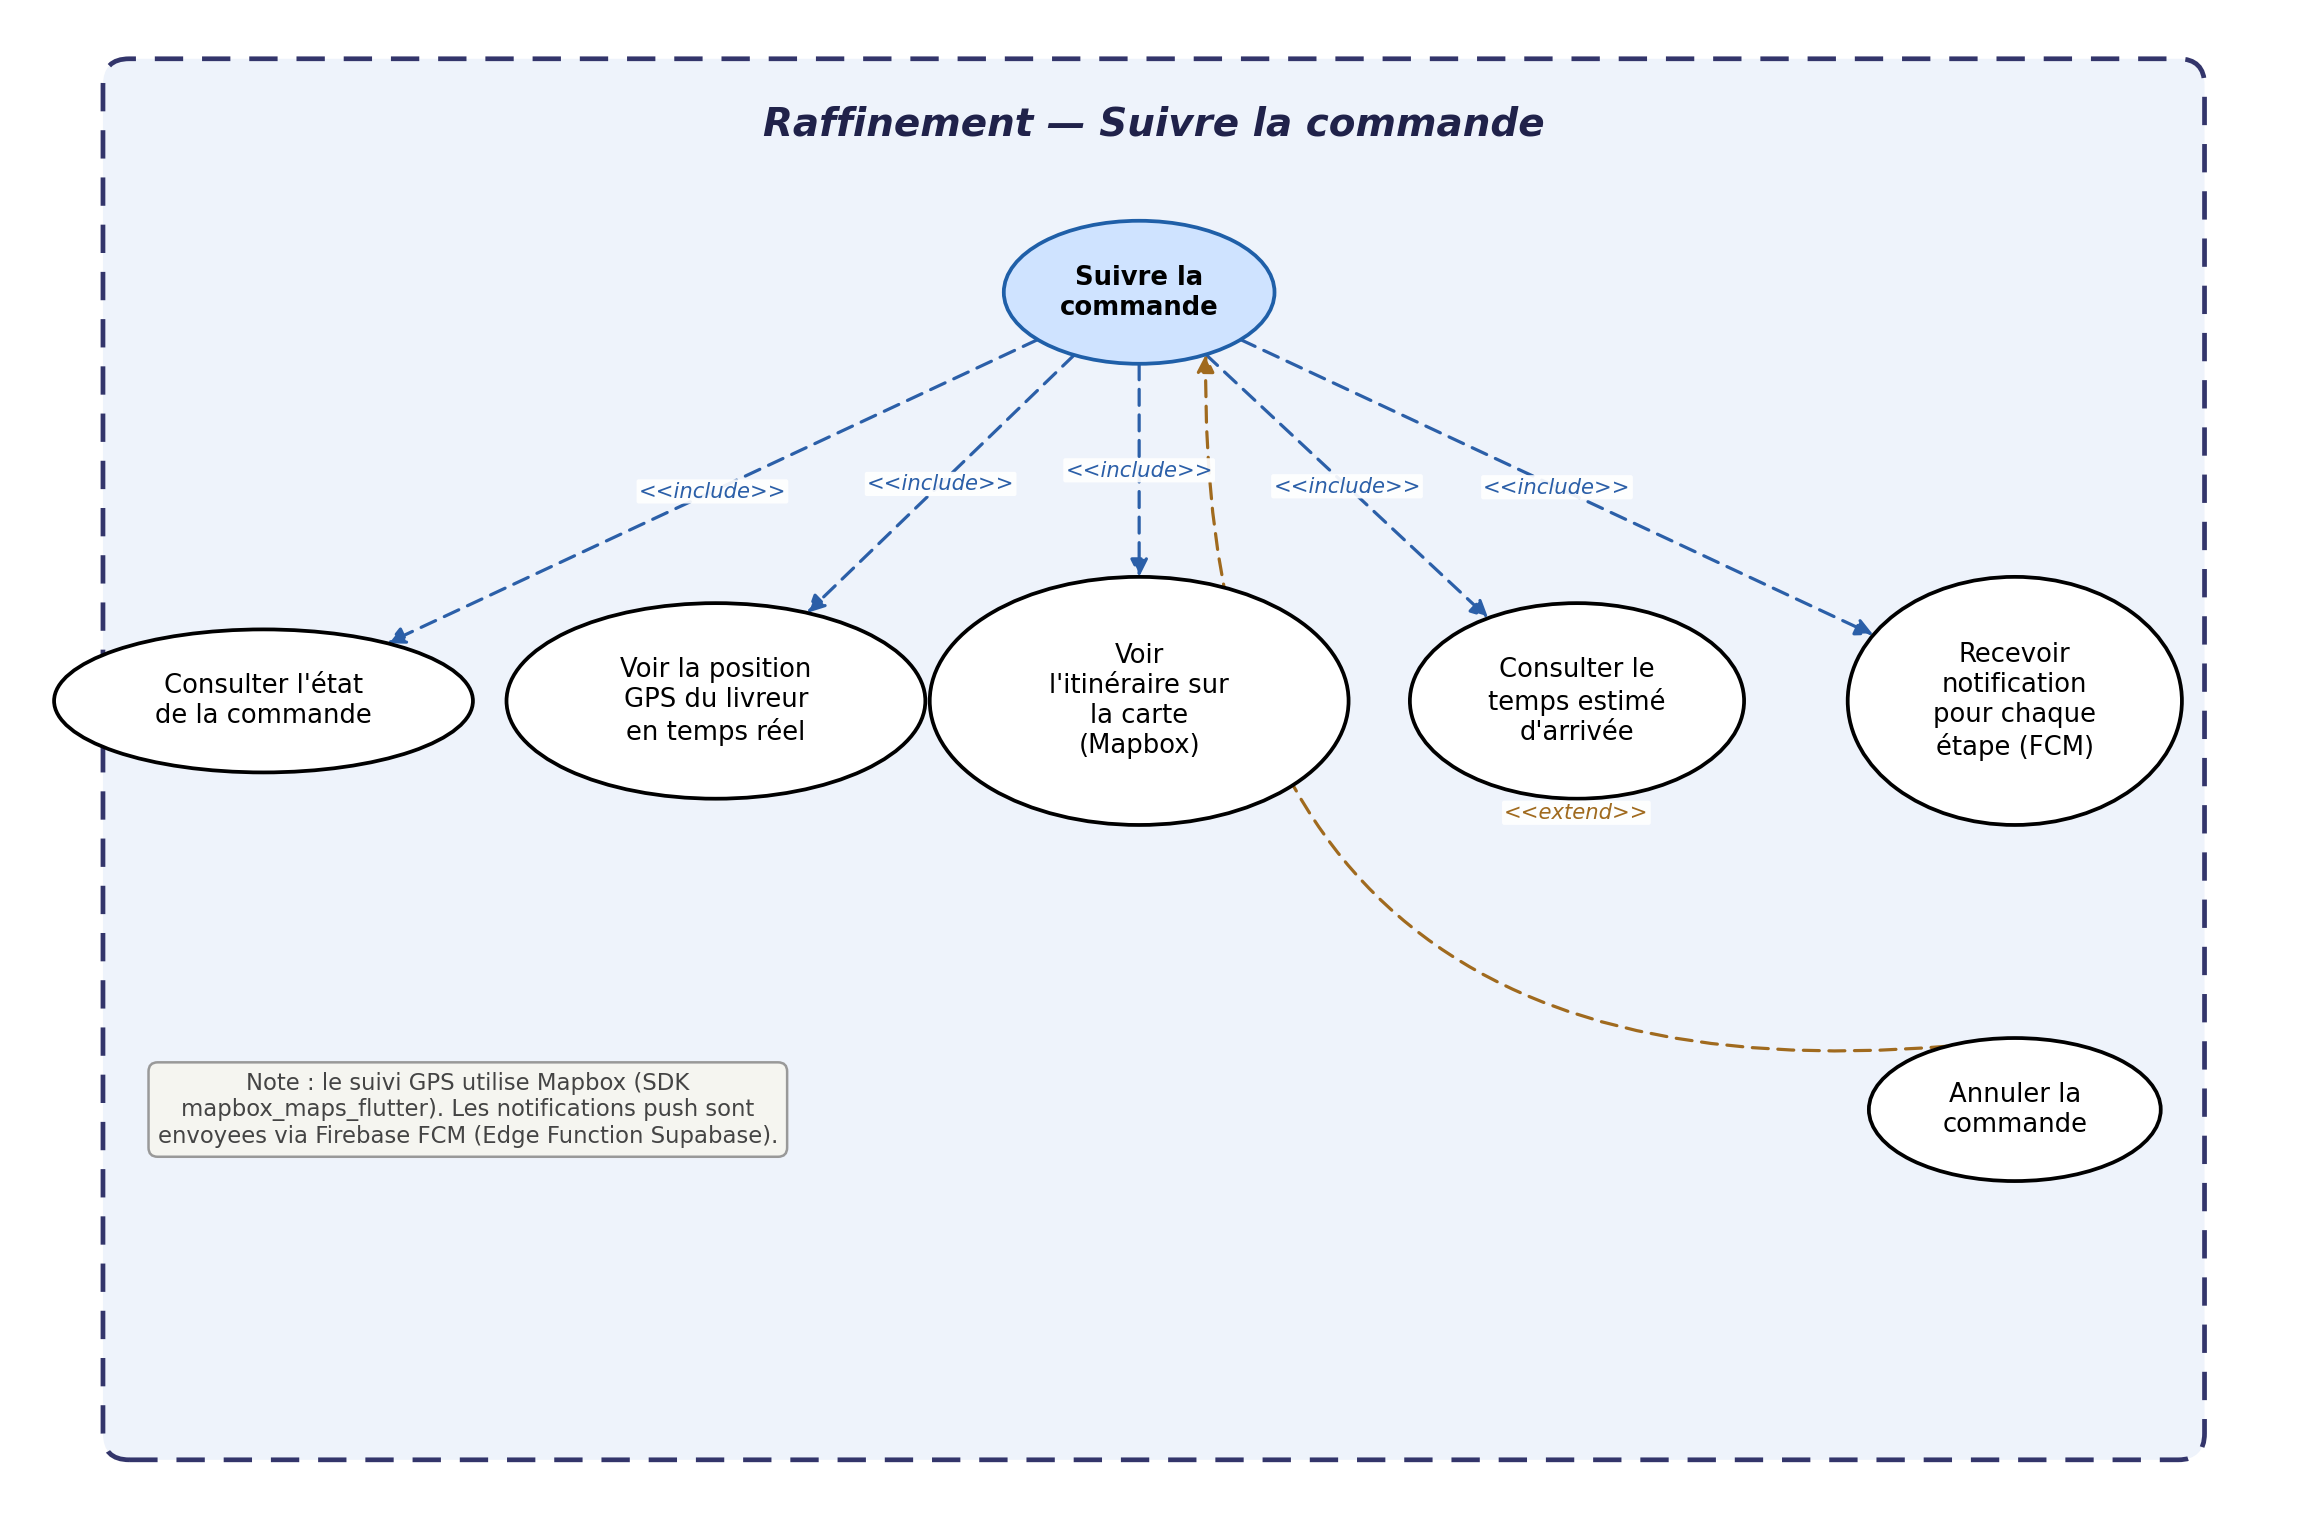
\includegraphics[width=\textwidth,height=0.6\textheight,keepaspectratio]{raffinement_suivre_commande_v2.png}}
    \caption{Raffinement du cas d'utilisation~: suivre une commande}
\end{figure}

\begin{table}[H]
\centering
\renewcommand{\arraystretch}{1.4}
\begin{tabular}{|l|l|p{7cm}|}
\hline
\textbf{Cas d'utilisation} & \textbf{Type} & \textbf{Description} \\
\hline
Suivre la commande & Cas principal &
Le client dispose d'un écran dédié pour surveiller en direct l'avancement de sa livraison. \\
\hline
Consulter l'état de la commande & Inclusion &
Un indicateur de progression affiche l'étape en cours parmi les huit statuts possibles du système, de la confirmation jusqu'à la livraison finale. \\
\hline
Voir la position GPS du livreur & Inclusion &
La position du livreur est mise à jour à chaque déplacement d'environ 30 mètres et apparaît sous forme de marqueur mobile sur la carte. \\
\hline
Voir l'itinéraire sur la carte & Inclusion &
Le trajet entre le livreur et le point de livraison est dessiné automatiquement via le SDK Mapbox. \\
\hline
Consulter le temps estimé d'arrivée & Extension &
À partir de la position GPS actuelle du livreur, le système calcule une durée approximative avant l'arrivée. \\
\hline
Recevoir une notification à chaque étape & Inclusion &
À chaque changement de statut, une alerte est envoyée sur le téléphone du client via Firebase FCM. \\
\hline
Annuler la commande & Extension &
Tant que la commande n'a pas été prise en charge, le client peut l'annuler en indiquant la raison de sa décision. \\
\hline
\end{tabular}
\caption{Description textuelle du raffinement~: suivre une commande}
\end{table}

Ce cas d'utilisation regroupe, autour d'un seul écran, des informations qui viennent de sources différentes~: le statut de la commande stocké en base, la position GPS du livreur transmise en direct, et l'itinéraire calculé par le service de cartographie. C'est cette combinaison qui rend le suivi utile pour le client.

\subsection{Livraison d'une commande}

\begin{figure}[H]
    \centering
    \fbox{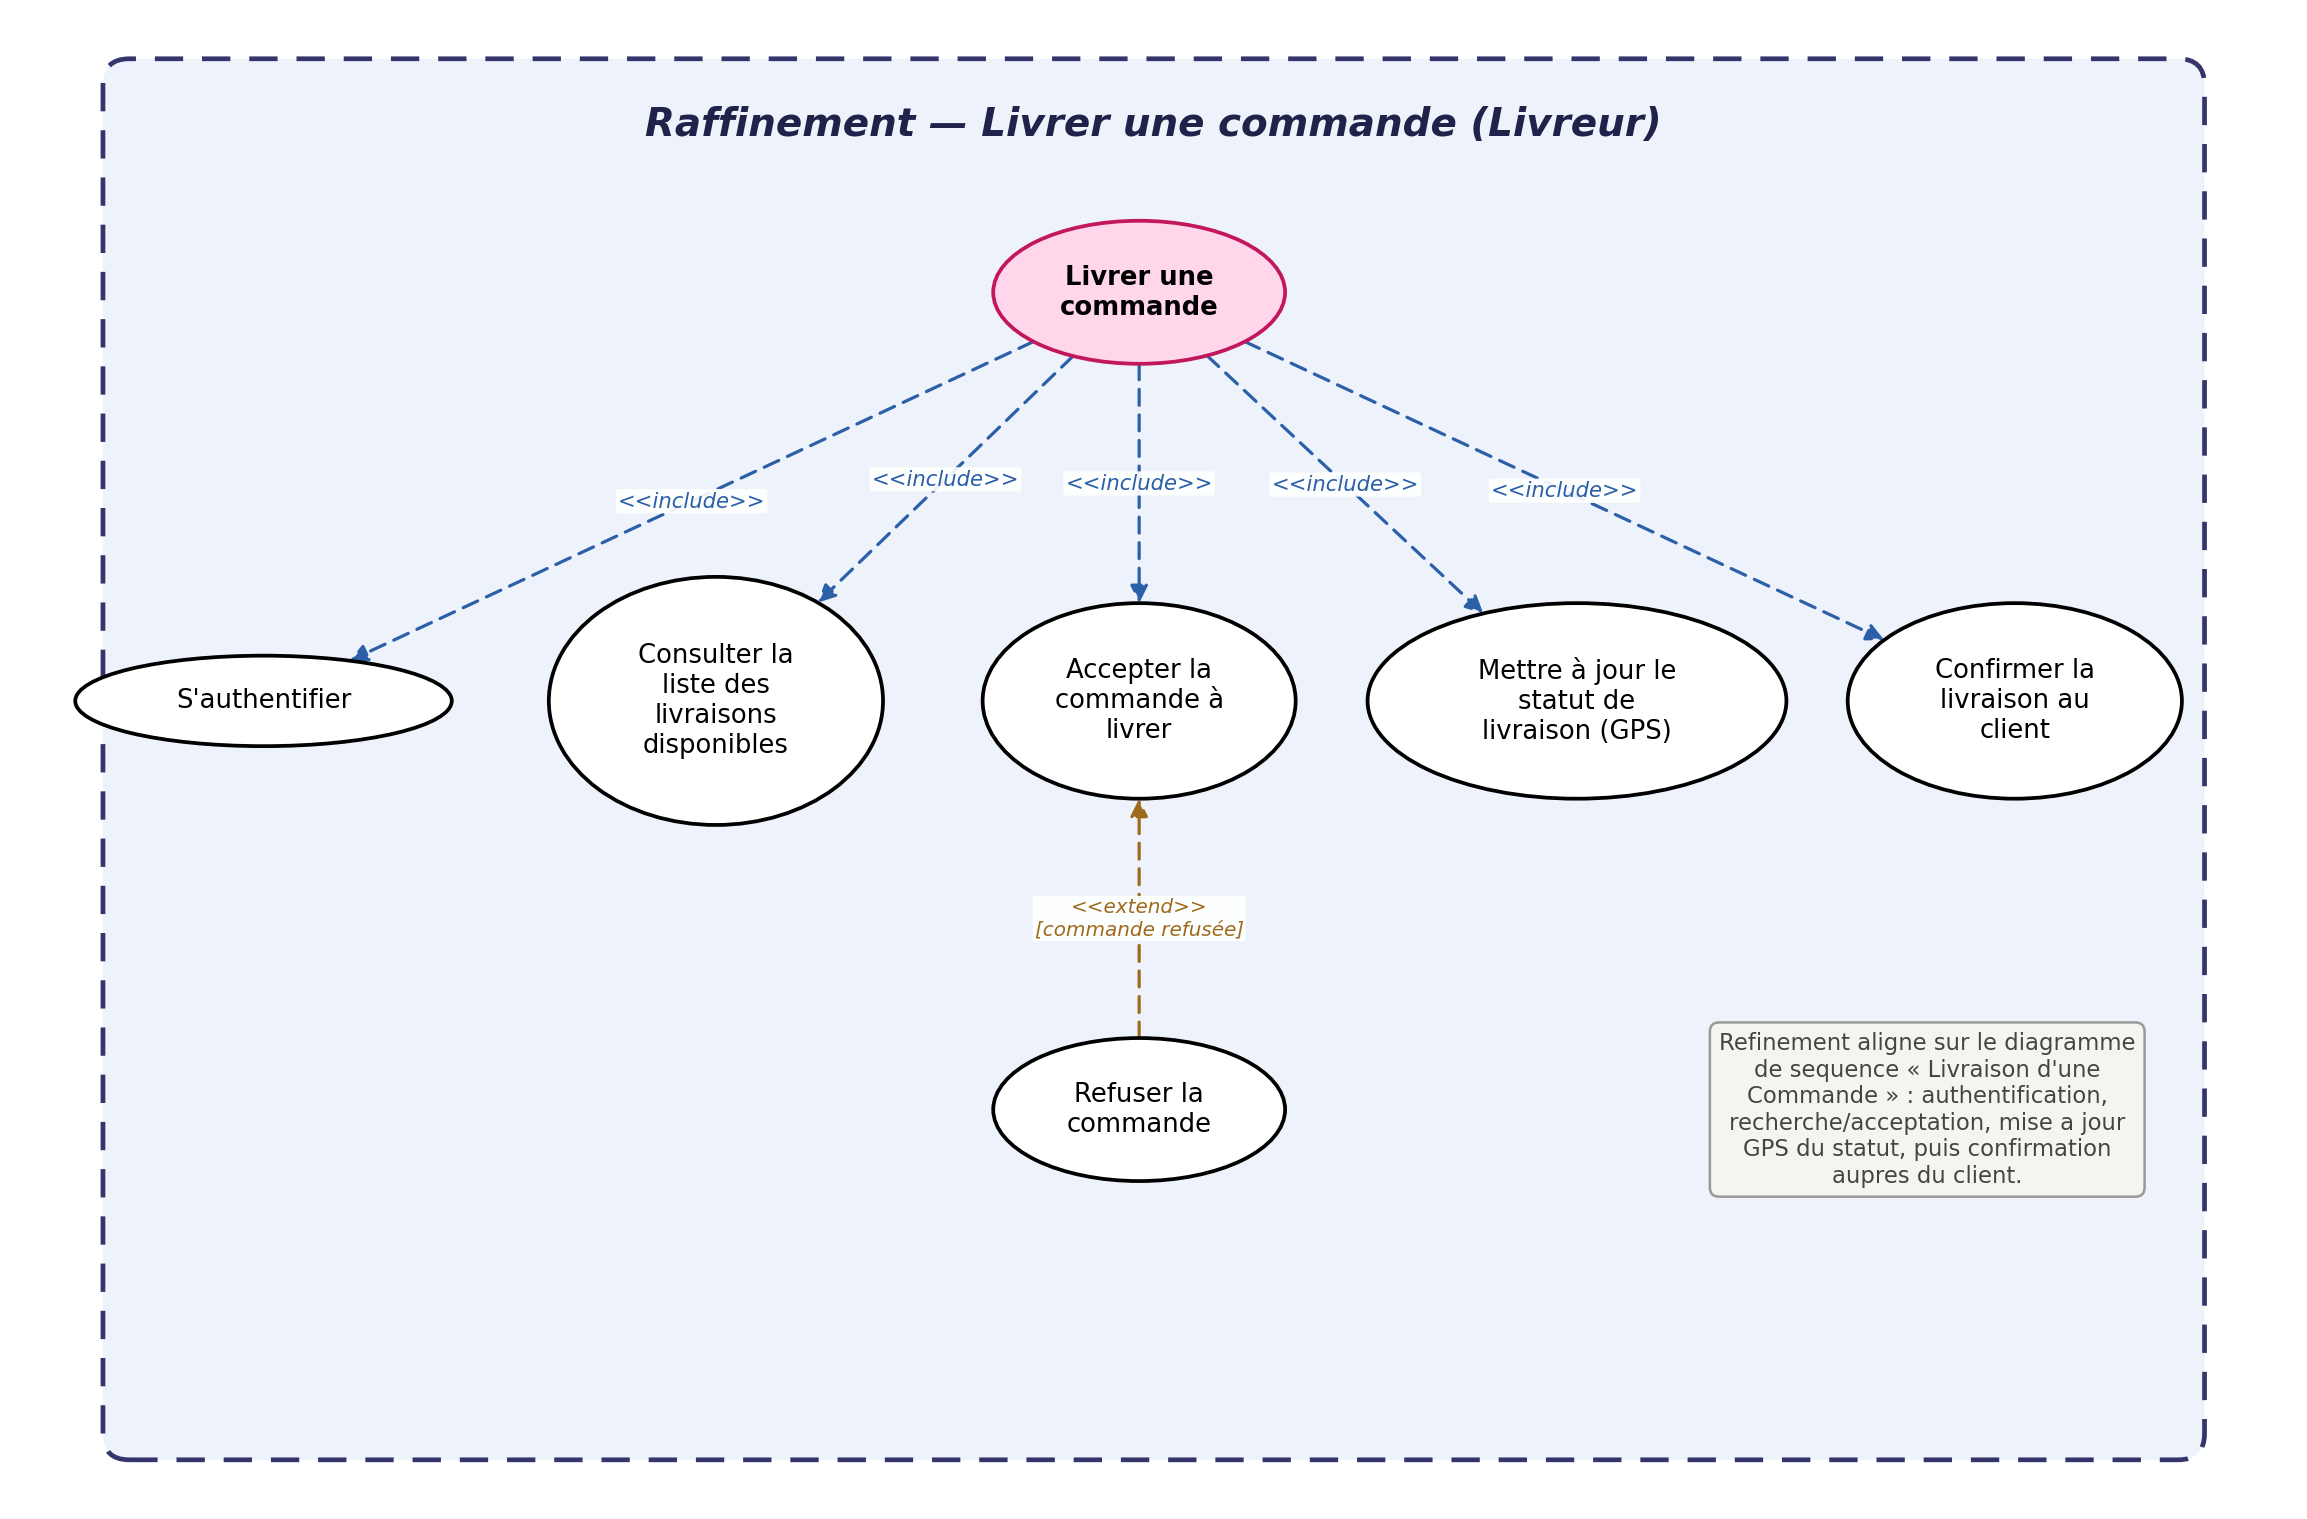
\includegraphics[width=\textwidth,height=0.6\textheight,keepaspectratio]{raffinement_livraison_commande.png}}
    \caption{Raffinement du cas d'utilisation~: livrer une commande}
\end{figure}

\begin{longtable}{|l|l|p{8cm}|}
\hline
\textbf{Cas d'utilisation} & \textbf{Type} & \textbf{Description} \\
\hline
\endfirsthead
\hline
\textbf{Cas d'utilisation} & \textbf{Type} & \textbf{Description} \\
\hline
\endhead
\hline
\endfoot
\hline
\caption{Description textuelle du raffinement~: livrer une commande}
\label{tab:raffinement_livrer}
\endlastfoot

Livrer une commande & Cas principal &
Le livreur prend en charge une commande validée par le commerçant, puis l'achemine jusqu'au client. \\
\hline
S'authentifier & Inclusion &
Le livreur se connecte à son compte, ce qui donne accès à son profil et à son état de disponibilité. \\
\hline
Consulter les livraisons disponibles & Inclusion &
L'application affiche les commandes proposées, avec le commerçant, l'adresse du client et le montant de la course. \\
\hline
Accepter la commande & Inclusion &
Le livreur confirme une offre, qui lui est alors attribuée et disparaît de la liste proposée aux autres livreurs. \\
\hline
Refuser la commande & Extension &
Si le livreur décline l'offre, elle est aussitôt proposée à un autre livreur disponible à proximité. \\
\hline
Mettre à jour le statut de livraison & Inclusion &
Pendant le trajet, la position du livreur est transmise régulièrement, et le statut de la commande évolue (ramassée, en route). \\
\hline
Confirmer la livraison & Inclusion &
À l'arrivée, le livreur valide la remise de la commande, ce qui déclenche l'ajout de sa rémunération au solde de son portefeuille. \\
\hline
\end{longtable}

La partie la plus délicate de ce cas d'utilisation concerne l'attribution de la commande~: comme le montre le raffinement, un refus n'arrête pas le processus, il le relance simplement vers un autre livreur. Ce mécanisme d'attribution en cascade, détaillé dans la section~\ref{sec:sequences} et implémenté au chapitre~3, est ce qui évite qu'une commande reste bloquée si le premier livreur sollicité ne répond pas.

\subsection{Ajout d'un plat du jour}

\begin{figure}[H]
    \centering
    \fbox{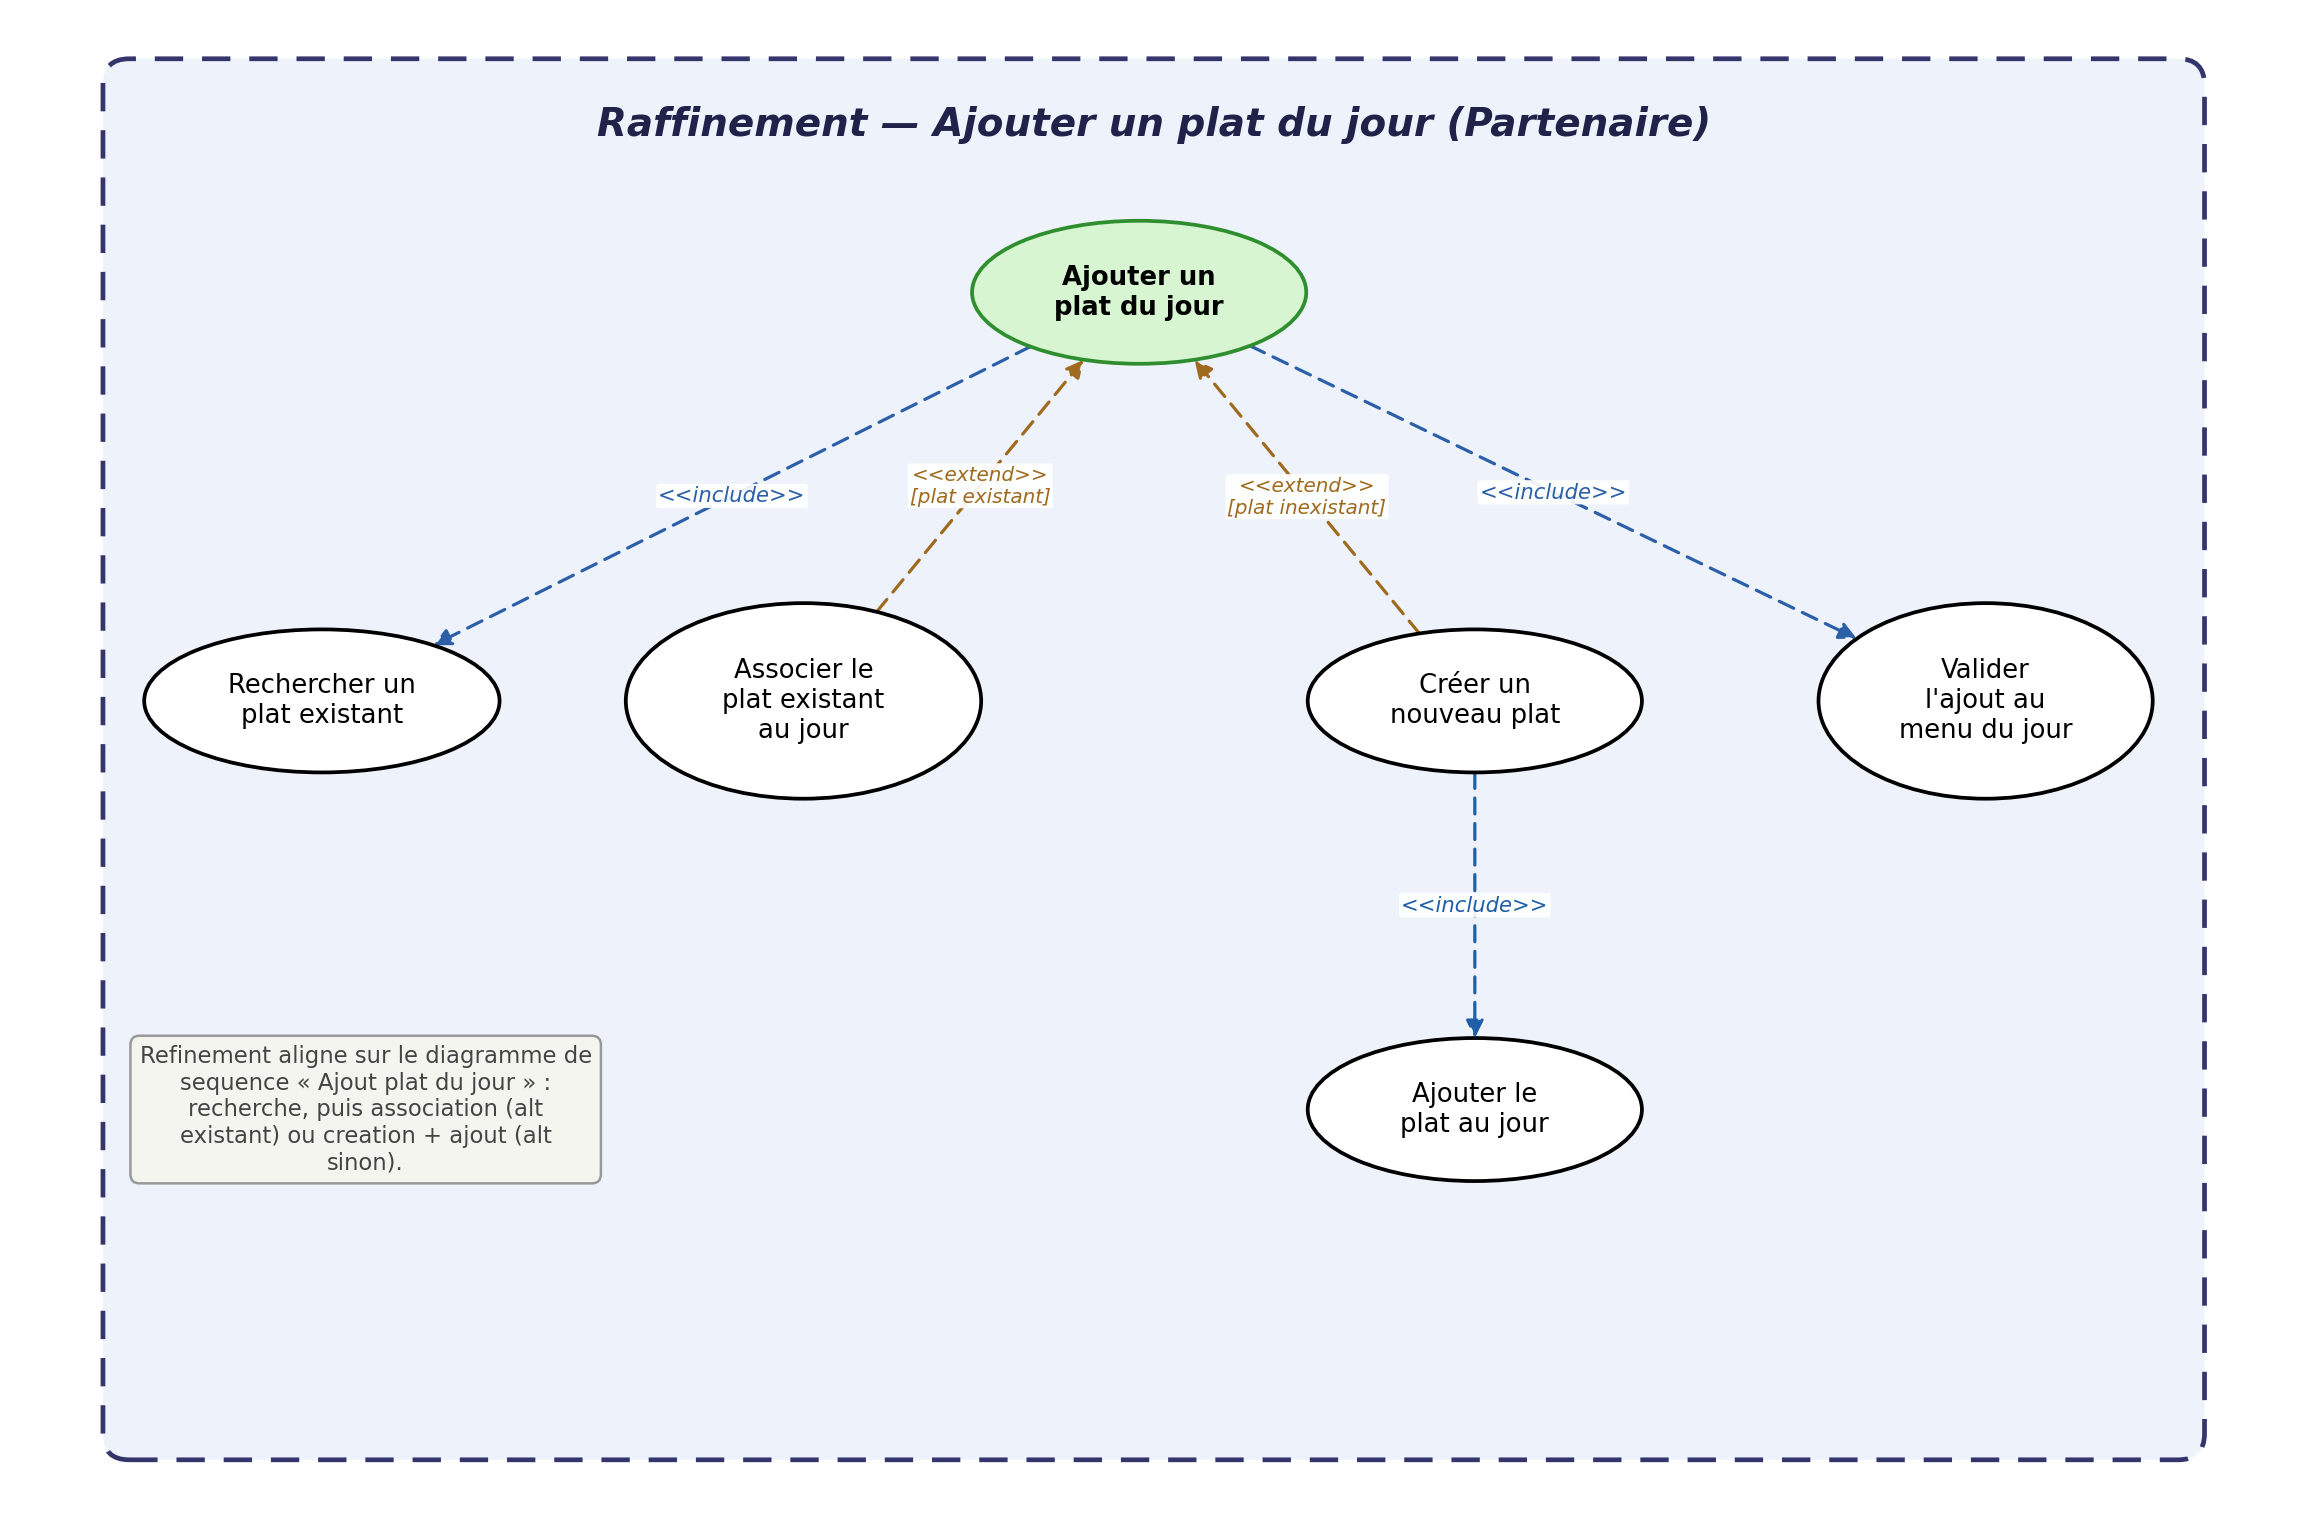
\includegraphics[width=\textwidth,height=0.7\textheight,keepaspectratio]{raffinement_ajout_plat_jour.png}}
    \caption{Raffinement du cas d'utilisation~: ajouter un plat du jour}
\end{figure}

\begin{table}[H]
\centering
\renewcommand{\arraystretch}{1.4}
\begin{tabular}{|l|l|p{8cm}|}
\hline
\textbf{Cas d'utilisation} & \textbf{Type} & \textbf{Description} \\
\hline
Ajouter un plat du jour & Cas principal &
Le partenaire met en avant un plat pour la journée, visible ensuite dans une section spéciale de l'application côté client. \\
\hline
Rechercher un plat existant & Inclusion &
L'application vérifie automatiquement si le plat existe déjà dans le menu du partenaire, pour éviter les doublons. \\
\hline
Associer le plat existant au jour & Extension &
Si le plat existe déjà, le partenaire le sélectionne et le rattache directement à la date du jour. \\
\hline
Créer un nouveau plat & Extension &
Si le plat n'existe pas encore, le partenaire saisit son nom, son prix, sa catégorie et une photo. \\
\hline
Valider l'ajout au menu du jour & Inclusion &
Le partenaire confirme son choix, et le plat devient visible côté client via Supabase Realtime. \\
\hline
\end{tabular}
\caption{Description textuelle du raffinement~: ajouter un plat du jour}
\end{table}

Ce cas d'utilisation illustre un choix de conception simple mais utile~: plutôt que d'obliger le partenaire à ressaisir un plat déjà existant, le système vérifie d'abord le menu et propose de réutiliser une fiche existante. Cela réduit les doublons dans le catalogue, un problème fréquent dans ce genre d'application.

\subsection{Envoi d'un colis}

Ce cas d'utilisation permet à un client d'envoyer un colis à une autre personne sans passer par un commerçant. Le client indique l'adresse de récupération, l'adresse de dépôt, les numéros de téléphone de l'expéditeur et du destinataire, ainsi qu'une description du colis. Contrairement aux commandes classiques, ce type de demande ne suit pas le mécanisme d'attribution automatique à un livreur précis~: elle apparaît directement dans la liste des commandes disponibles, et c'est un livreur qui choisit de l'accepter.

\begin{table}[H]
\centering
\renewcommand{\arraystretch}{1.4}
\begin{tabular}{|l|l|p{7cm}|}
\hline
\textbf{Cas d'utilisation} & \textbf{Type} & \textbf{Description} \\
\hline
Envoyer un colis & Cas principal &
Le client crée une demande de transport d'un colis entre deux adresses, sans commerçant impliqué. \\
\hline
Estimer le prix & Inclusion &
L'application calcule automatiquement un tarif, à partir d'un montant fixe majoré selon la distance. \\
\hline
Joindre une photo du colis & Extension &
Le client peut ajouter une photo pour faciliter l'identification du colis par le livreur. \\
\hline
Mémoriser le destinataire & Extension &
Le client peut enregistrer le destinataire pour de futurs envois. \\
\hline
\end{tabular}
\caption{Description textuelle du cas d'utilisation~: envoi d'un colis}
\end{table}

\section{Architecture générale du système}

\subsection{Architecture client-serveur}

L'architecture de la plateforme Amana repose sur un modèle client-serveur enrichi par des événements en temps réel. Le système est découpé en quatre couches qui communiquent entre elles de manière structurée.

La plateforme se compose de quatre applications indépendantes qui partagent un seul backend centralisé, comme le montre le tableau~\ref{tab:quatre_apps}.

\begin{table}[H]
\centering
\renewcommand{\arraystretch}{1.4}
\begin{tabular}{|l|l|l|}
\hline
\textbf{Application} & \textbf{Technologie} & \textbf{Utilisateur cible} \\
\hline
Application client & Flutter & Client final \\
\hline
Application livreur & Flutter & Livreur \\
\hline
Application partenaire & Flutter & Restaurant / Commerce \\
\hline
Tableau de bord admin & Next.js & Administrateur \\
\hline
\end{tabular}
\caption{Les quatre applications de la plateforme Amana}
\label{tab:quatre_apps}
\end{table}

\textbf{Couche présentation~:} elle regroupe les interfaces avec lesquelles l'utilisateur interagit. Les trois applications mobiles sont développées en Flutter, ce qui permet une seule base de code pour Android et iOS. Le tableau de bord administratif est une application web développée avec Next.js, accessible depuis un navigateur.

\vspace{0.3cm}
\textbf{Couche backend~:} entièrement gérée par Supabase, qui regroupe plusieurs services (tableau~\ref{tab:backend}).

\begin{table}[H]
\centering
\renewcommand{\arraystretch}{1.4}
\begin{tabular}{|l|l|}
\hline
\textbf{Service} & \textbf{Rôle} \\
\hline
PostgreSQL 17.6 & Stockage de toutes les données métier \\
\hline
Supabase Auth & Gestion de l'authentification et des sessions \\
\hline
Supabase Realtime & Synchronisation instantanée entre les applications \\
\hline
Edge Functions & Traitement serveur sans infrastructure à gérer \\
\hline
Row Level Security (RLS) & Contrôle d'accès aux données par rôle utilisateur \\
\hline
\end{tabular}
\caption{Services backend utilisés via Supabase}
\label{tab:backend}
\end{table}

\vspace{0.3cm}
\textbf{Couche services externes~:} certaines fonctionnalités nécessitent des services tiers spécialisés (tableau~\ref{tab:externes}).

\begin{table}[H]
\centering
\renewcommand{\arraystretch}{1.4}
\begin{tabular}{|l|l|}
\hline
\textbf{Service} & \textbf{Utilisation} \\
\hline
Firebase FCM & Envoi des notifications push \\
\hline
Mapbox & Affichage des cartes et suivi GPS en temps réel \\
\hline
OpenRouter / Gemini & Assistant conversationnel et recherche intelligente \\
\hline
\end{tabular}
\caption{Services externes intégrés dans la plateforme}
\label{tab:externes}
\end{table}

Le schéma suivant illustre comment les données circulent entre les couches lors d'une commande type~:

\begin{enumerate}
    \item le client passe une commande depuis l'application mobile~;
    \item la requête est transmise au backend Supabase via l'API REST~;
    \item la base de données enregistre la commande et déclenche automatiquement un processus d'attribution à un livreur~;
    \item l'application du livreur reçoit la nouvelle offre en temps réel via Supabase Realtime~;
    \item une fois la commande acceptée, la position GPS du livreur est transmise à chaque déplacement d'environ 30 mètres~;
    \item le client visualise la progression de sa livraison en direct sur la carte Mapbox.
\end{enumerate}

Ce choix architectural présente plusieurs avantages~: un seul point de gestion pour quatre applications, une synchronisation instantanée essentielle pour une plateforme de livraison, un contrôle d'accès géré directement au niveau de la base de données grâce à RLS, et une capacité à absorber une montée en charge sans changement d'infrastructure majeur grâce aux Edge Functions.

\subsection{Architecture des applications mobiles}

Les trois applications mobiles (Client, Livreur, Partenaire) suivent le patron \textbf{MVVM} (\textit{Model-View-ViewModel}), qui répartit le code en trois responsabilités.

\begin{itemize}
    \item \textbf{M — Model~:} les données manipulées par l'application et les traitements qui les concernent, sans lien avec leur affichage.
    \item \textbf{V — View~:} ce que l'utilisateur voit à l'écran. Son rôle se limite à présenter les informations reçues et à transmettre les actions effectuées.
    \item \textbf{VM — ViewModel~:} la position intermédiaire. Il récupère les données du modèle, les met en forme pour l'affichage et expose l'état courant de l'interface.
\end{itemize}

L'intérêt de ce découpage est l'absence de lien direct entre la vue et le modèle~: la vue observe le \textit{ViewModel} et se redessine quand l'état change, sans jamais interroger elle-même la source des données. Il devient possible de modifier l'apparence d'un écran sans toucher à la logique qui l'alimente.

\begin{table}[H]
\centering
\renewcommand{\arraystretch}{1.4}
\begin{tabular}{|l|l|l|}
\hline
\textbf{Composante} & \textbf{Rôle} & \textbf{Exemple dans les apps mobiles Amana} \\
\hline
Model & Données et logique métier & Dossier \texttt{data/} (modèles + repository Supabase) \\
\hline
View & Interface utilisateur & Dossier \texttt{presentation/} (écrans et widgets Flutter) \\
\hline
ViewModel & État et logique d'affichage & Dossier \texttt{providers/} (Riverpod) \\
\hline
\end{tabular}
\caption{Manifestation du patron MVVM dans les applications mobiles Amana}
\end{table}

Il n'existe pas de classe \textit{ViewModel} séparée dans le code~: c'est directement le \textit{provider} Riverpod qui joue ce rôle intermédiaire entre les données et l'écran. L'organisation concrète des dossiers est détaillée au chapitre~3.

\subsection{Architecture de l'application web}

Le tableau de bord administratif suit, lui, le patron \textbf{MVC} (\textit{Modèle -- Vue -- Contrôleur}), plus adapté à une architecture Next.js basée sur des routes API.

\begin{itemize}
    \item \textbf{M — Modèle~:} représente la couche des données et de la logique métier.
    \item \textbf{V — Vue~:} constitue la couche de présentation, sans logique applicative.
    \item \textbf{C — Contrôleur~:} joue le rôle d'intermédiaire entre le modèle et la vue.
\end{itemize}

\begin{table}[H]
\centering
\renewcommand{\arraystretch}{1.4}
\begin{tabular}{|l|l|l|}
\hline
\textbf{Composante} & \textbf{Rôle} & \textbf{Exemple dans le tableau de bord Amana} \\
\hline
Modèle & Données et logique métier & PostgreSQL, tables \texttt{orders}, RLS \\
\hline
Vue & Interface utilisateur & Composants React, \texttt{app/dashboard/} \\
\hline
Contrôleur & Traitement des requêtes & Routes API, \texttt{app/api/loyalty/settle} \\
\hline
\end{tabular}
\caption{Manifestation du patron MVC dans le tableau de bord Amana}
\end{table}

Dans ce découpage, la base de données \textbf{PostgreSQL} gérée par Supabase constitue la couche données~: les tables \texttt{orders}, \texttt{drivers}, \texttt{restaurants} et \texttt{food\_items} centralisent l'information métier, avec les règles RLS et les triggers associés. Les composants \textbf{React} du répertoire \texttt{app/dashboard/} forment la couche vue~: ils affichent les statistiques, les listes de commandes et les rapports financiers, sans logique de traitement. Les routes \textbf{API} de \texttt{app/api/} jouent le rôle de contrôleurs~: par exemple, \texttt{/api/loyalty/settle} traite le règlement des primes des livreurs, et \texttt{/api/restaurants/categories} gère les catégories de restaurants. Chaque route vérifie d'abord l'identité de l'administrateur via la fonction \texttt{requireAdmin()}, avant d'interagir avec Supabase.

Les pages du tableau de bord sont organisées par domaine fonctionnel, comme le montre le tableau~\ref{tab:pages_admin}.

\begin{table}[H]
\centering
\renewcommand{\arraystretch}{1.4}
\begin{tabular}{|l|l|}
\hline
\textbf{Section} & \textbf{Fonctionnalités} \\
\hline
Tableau de bord principal & Statistiques en temps réel, revenus, commandes actives \\
\hline
Gestion des commandes & Suivi, recherche, annulation, historique \\
\hline
Gestion des livreurs & Liste, statut en ligne, règlement des paiements \\
\hline
Gestion des restaurants & Ajout, modification, catégories, disponibilité \\
\hline
Gestion des clients & Profils, historique des commandes \\
\hline
Finances & Commissions, relevés, export PDF et CSV \\
\hline
Fidélité & Tableau de bord des récompenses et règlements livreurs \\
\hline
Paramètres & Codes promo, configuration générale \\
\hline
\end{tabular}
\caption{Organisation fonctionnelle du tableau de bord}
\label{tab:pages_admin}
\end{table}

\subsection{Communication avec le back-end}

Les quatre applications communiquent avec Supabase via deux canaux complémentaires. L'\textbf{API REST} est utilisée pour les opérations classiques~: création d'une commande, mise à jour d'un profil, récupération d'une liste de restaurants. Le \textbf{WebSocket Supabase Realtime} est utilisé pour les mises à jour instantanées~: la position du livreur sur la carte, ou l'arrivée d'une nouvelle commande chez le partenaire. Côté tableau de bord administrateur, Supabase Realtime est utilisé sur la page des commandes, où les nouvelles commandes et les changements de statut apparaissent automatiquement, sans que l'administrateur ait besoin de recharger la page.

\section{Modélisation des données}

\subsection{Diagramme de classes}

Le diagramme de classes ci-dessous regroupe l'ensemble des entités du projet Amana. On y retrouve les acteurs (Client, Livreur), les partenaires commerciaux, les commandes et leurs lignes, ainsi que les articles proposés à la vente (produits et plats). Trois types de relations sont utilisés~: l'héritage relie les sous-classes à une classe abstraite commune, la composition et l'agrégation expriment des liens de dépendance entre entités, et l'association simple relie deux classes indépendantes.

\begin{landscape}
\begin{figure}[p]
    \centering
    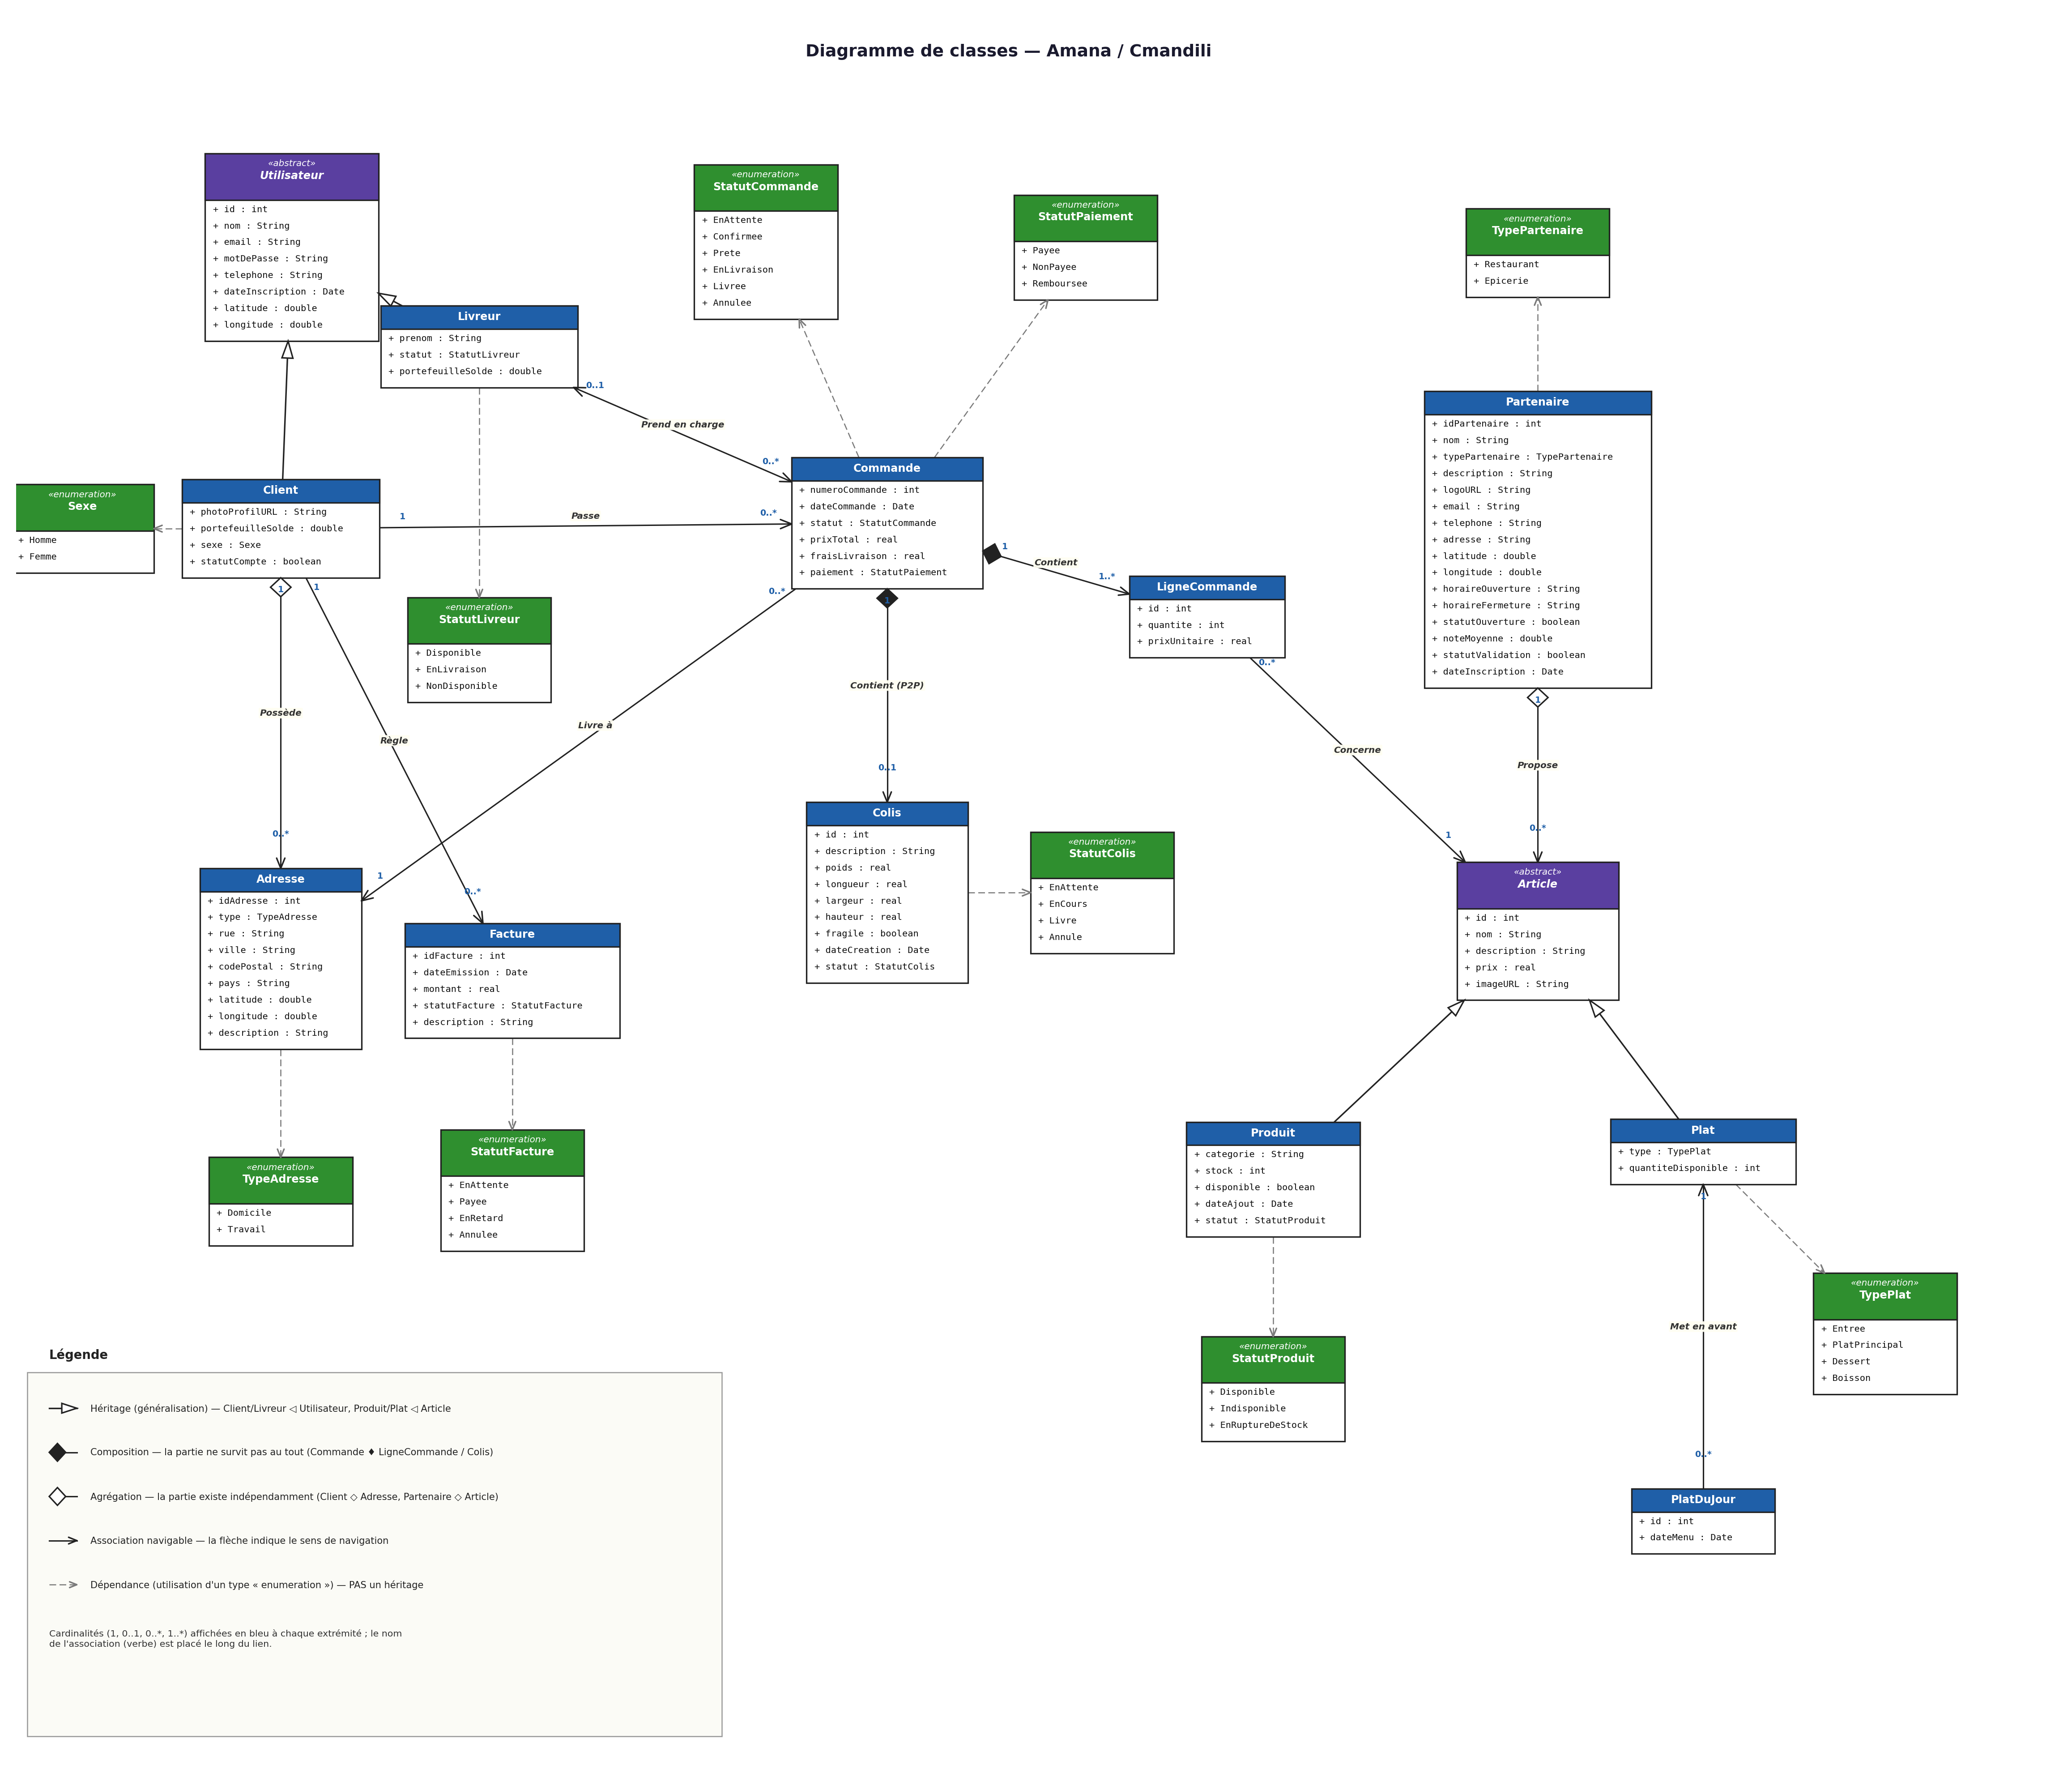
\includegraphics[width=\linewidth,keepaspectratio]{diagramme_classe_v2_full.png}
    \caption{Diagramme de classes de la plateforme Amana}
    \label{fig:diagramme_classe}
\end{figure}
\end{landscape}
\newpage

Ce diagramme sert de base directe à la conception de la base de données PostgreSQL~: chaque classe correspond, dans les grandes lignes, à une table relationnelle. Le tableau~\ref{tab:classes} résume le rôle de chacune des classes principales.

\subsection{Description des principales classes}

\begin{longtable}{|l|p{9cm}|}
\hline
\textbf{Classe} & \textbf{Rôle dans le système} \\
\hline
\endfirsthead
\hline
\textbf{Classe} & \textbf{Rôle dans le système} \\
\hline
\endhead
\hline
\endfoot
\hline
\caption{Description des principales classes du système}
\label{tab:classes}
\endlastfoot

Utilisateur &
Classe abstraite qui regroupe les informations communes à toute personne inscrite sur la plateforme, comme le nom, l'e-mail et la position géographique. Les classes Client et Livreur en héritent. \\
\hline
Client &
Représente la personne qui passe des commandes. Elle possède une ou plusieurs adresses et peut régler ses factures. \\
\hline
Livreur &
Représente la personne chargée d'acheminer les commandes. Son statut de disponibilité change selon qu'il est libre, en livraison ou indisponible, et il dispose d'un solde de portefeuille. \\
\hline
Adresse &
Décrit un lieu de livraison ou de facturation lié à un client, avec ses coordonnées postales et géographiques. \\
\hline
Facture &
Représente le document financier émis pour une commande, avec son montant et son état de paiement. \\
\hline
Commande &
Classe centrale du système. Elle regroupe les informations générales d'un achat~: prix total, frais de livraison, état d'avancement. Elle peut être prise en charge par un livreur. \\
\hline
LigneCommande &
Représente un article précis inclus dans une commande, avec la quantité choisie et le prix appliqué au moment de l'achat. \\
\hline
Colis &
Représente une livraison de type colis à colis, indépendante des commandes classiques de produits ou de plats. \\
\hline
Partenaire &
Représente un commerçant inscrit sur la plateforme, restaurant ou épicerie. Il propose des articles à la vente et gère ses horaires d'ouverture. \\
\hline
Article &
Classe abstraite commune aux éléments proposés à la vente par un partenaire. Les classes Produit et Plat en héritent. \\
\hline
Produit &
Article de type épicerie, avec une gestion de stock et une disponibilité qui peut évoluer dans le temps. \\
\hline
Plat &
Article de type restauration, classé par catégorie (entrée, plat principal, dessert ou boisson). \\
\hline
PlatDuJour &
Met en avant un plat particulier pour une date précise, afin de le faire apparaître dans une section spéciale de l'application. \\
\hline
\end{longtable}

\subsection{Organisation de la base de données}

La base de données PostgreSQL est commune aux quatre applications~: elle regroupe les comptes utilisateurs, les restaurants et supermarchés, les produits, les commandes, les livraisons, les portefeuilles et commissions, le programme de fidélité et les codes promotionnels. Chaque application ne peut lire et modifier que les données qui la concernent, grâce aux règles de sécurité RLS définies sur chaque table~: un client ne voit jamais les commandes d'un autre client, un livreur ne voit que les commandes qui lui sont proposées ou attribuées, et ainsi de suite. Ce choix évite d'écrire cette logique de séparation dans chacune des quatre applications~: elle est centralisée une seule fois, au niveau de la base de données.

\section{Diagrammes de séquence}
\label{sec:sequences}

Les diagrammes de cas d'utilisation présentés plus haut décrivent \emph{ce que} le système permet de faire. Les diagrammes de séquence qui suivent décrivent \emph{comment}, dans le temps, les composants du système échangent des messages pour réaliser ces six mêmes scénarios.

\subsection{Authentification et inscription}

Trois chemins alternatifs sont possibles au départ. Dans le premier, l'utilisateur crée un nouveau compte en saisissant son nom, son e-mail et un mot de passe~; cette action déclenche la création d'un compte côté Supabase Auth, puis un déclencheur automatique insère son profil dans la base de données. Dans le deuxième chemin, un utilisateur déjà inscrit se connecte simplement avec son e-mail et son mot de passe. Le troisième chemin correspond à la connexion via Google~: l'application récupère un jeton d'identification, puis l'envoie à Supabase Auth pour ouvrir une session, sans mot de passe.

Une fois la session ouverte, l'application vérifie si un numéro de téléphone est déjà enregistré dans le profil. Si c'est le cas, l'accès est immédiat~; sinon, un écran obligatoire demande sa saisie, sans vérification par SMS. Enfin, un jeton de notification est associé au compte, ce qui permettra à l'application de transmettre des notifications push par la suite, en arrière-plan, dès que la session est confirmée.

\begin{figure}[H]
\centering
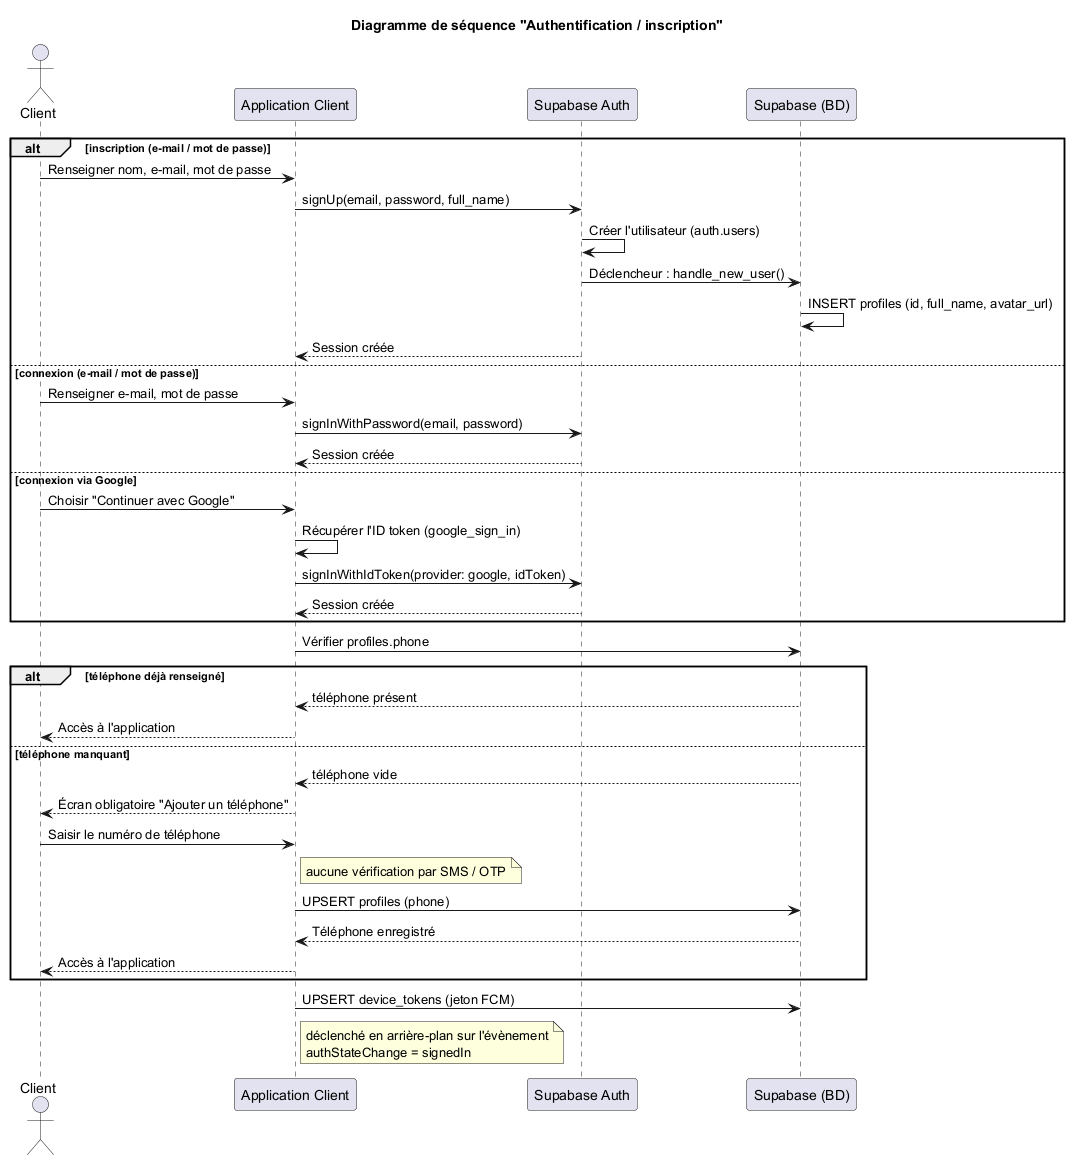
\includegraphics[width=\textwidth]{diagramme_sequence_authentification.png}
\caption{Diagramme de séquence — Authentification / inscription}
\label{fig:sequence_authentification}
\end{figure}

Ce diagramme montre que la création d'un compte et le renseignement du numéro de téléphone sont deux étapes distinctes~: la première est gérée entièrement par Supabase Auth, la seconde est propre à l'application Amana. Cette séparation permet de garder la partie authentification simple, tout en ajoutant une information métier supplémentaire sans modifier le fonctionnement standard de Supabase Auth.

\subsection{Création d'une commande}

Ce diagramme retrace les échanges entre le client, l'application, le serveur et la base de données pendant la constitution puis la validation d'une commande, dans la continuité du raffinement présenté à la section~2.4.2.

\begin{figure}[H]
    \centering
    \fbox{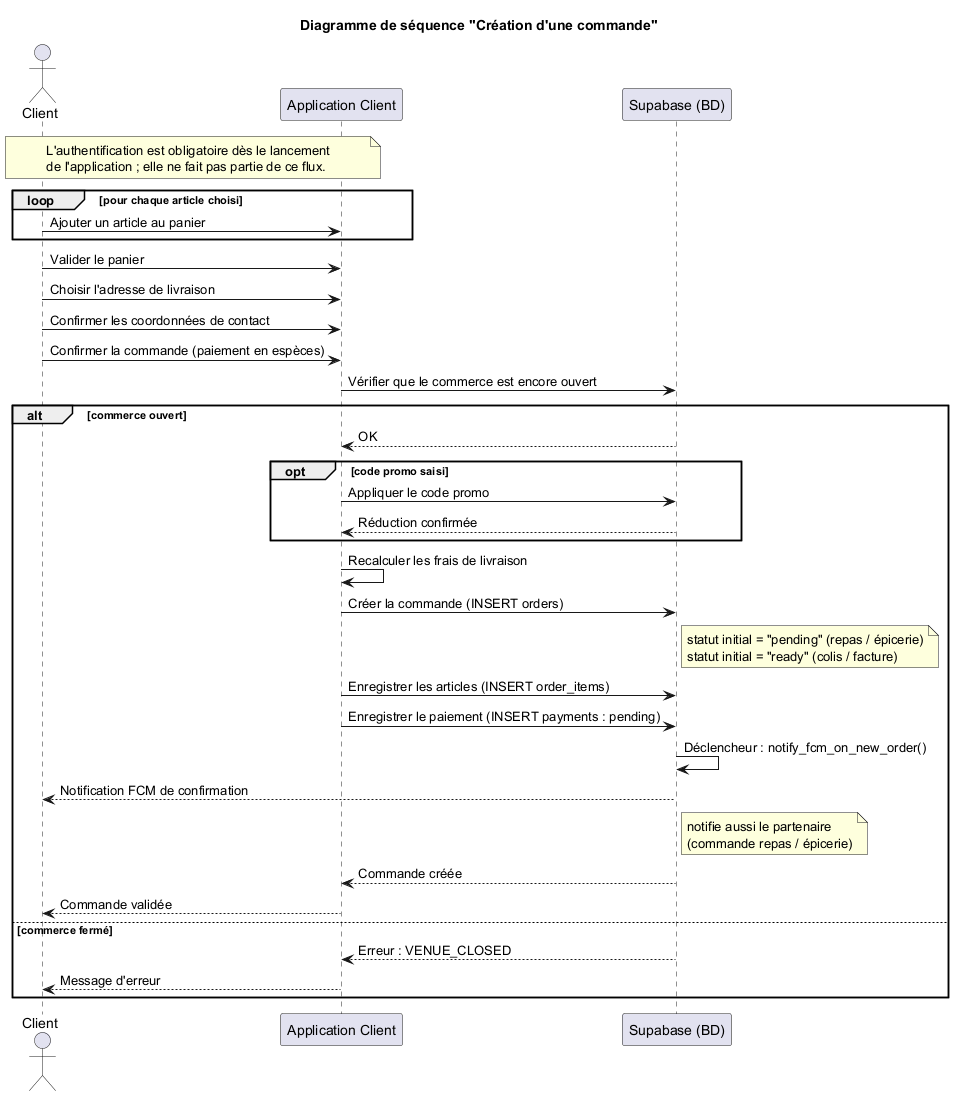
\includegraphics[width=17cm,height=24cm,keepaspectratio]{diagramme_sequence_creation_commande_v2.png}}
    \caption{Diagramme de séquence — Création d'une commande}
\end{figure}
\newpage

On y voit que la commande n'est écrite qu'une seule fois en base, au moment de la confirmation finale~: toutes les étapes précédentes (ajout au panier, choix de l'adresse, choix du paiement) restent locales à l'application, sur le téléphone du client. Ce choix évite de créer des commandes incomplètes ou abandonnées dans la base de données.

\newpage
\subsection{Livraison d'une commande}

Ce diagramme illustre le parcours du livreur, depuis la réception d'une offre de commande jusqu'à sa remise finale au client, dans la continuité du raffinement présenté à la section~2.4.4.

\begin{figure}[H]
    \centering
    \fbox{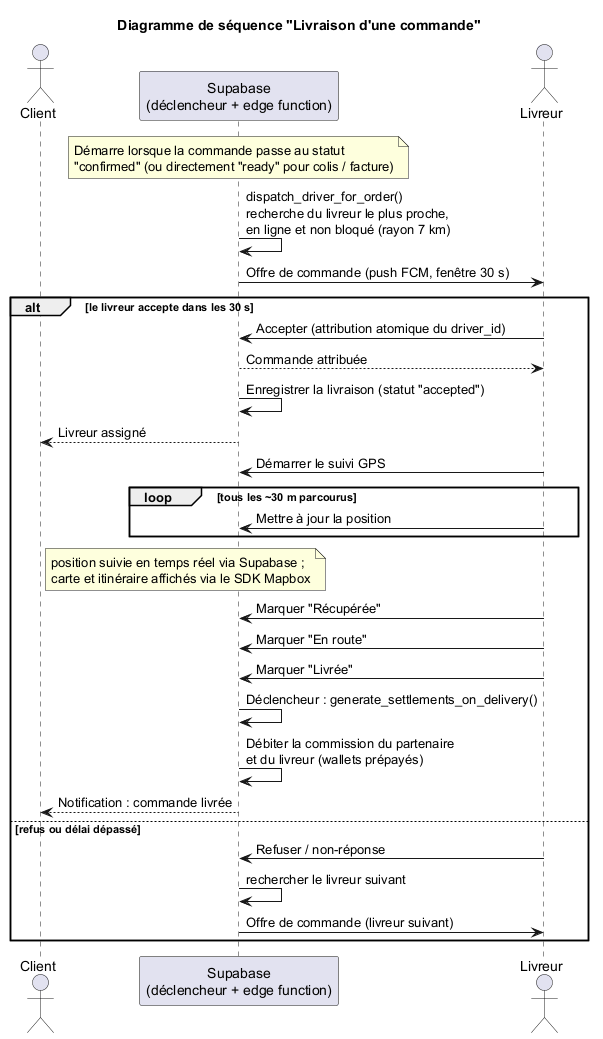
\includegraphics[width=17cm,height=21cm,keepaspectratio]{diagramme_sequence_livraison_commande_v2.png}}
    \caption{Diagramme de séquence — Livraison d'une commande}
\end{figure}
\newpage

Le point important de ce diagramme est le mécanisme d'attribution~: si le livreur sollicité ne répond pas dans le délai imparti, ou refuse explicitement, la commande est automatiquement proposée au livreur disponible suivant. Ce mécanisme, appelé dispatch en cascade, est implémenté côté serveur et détaillé au chapitre~3.

\subsection{Ajout d'un plat du jour}

Ce diagramme illustre le déroulement du cas d'utilisation présenté à la section~2.4.5, du point de vue du partenaire qui ajoute un plat à mettre en avant pour la journée.

\begin{figure}[H]
    \centering
    \fbox{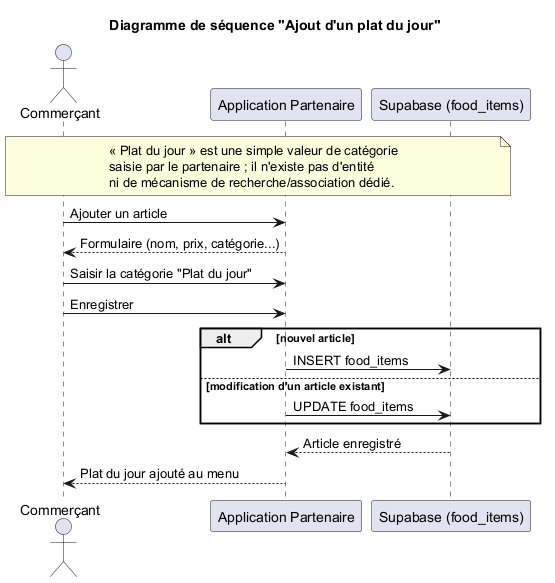
\includegraphics[width=15cm,height=21cm,keepaspectratio]{diagramme_sequence_ajout_plat_jour_v2.png}}
    \caption{Diagramme de séquence — Ajout d'un plat du jour}
\end{figure}
\newpage

Ce diagramme confirme que la vérification d'existence du plat se fait avant toute autre étape~: c'est ce contrôle préalable qui permet ensuite de proposer au partenaire deux chemins différents (réutiliser un plat existant ou en créer un nouveau), comme décrit dans le raffinement correspondant.

\subsection{Débit des commissions}

Ce diagramme décrit le mécanisme déclenché automatiquement lorsqu'une commande passe à l'état livrée, sans aucune action manuelle du livreur ou du partenaire.

Le comportement du système dépend du mode de paiement choisi par le client. Lorsque la commande a été réglée en espèces, un déclencheur calcule automatiquement les commissions dues, à partir d'un taux lu dans les paramètres globaux de la plateforme~: dix pour cent pour le partenaire et vingt-trois pour cent pour le livreur, par défaut. La commission du partenaire porte sur le montant des articles commandés, celle du livreur sur les frais de livraison~; cette dernière est nulle lorsque la livraison a été assurée directement par le commerçant. Ces montants sont ensuite déduits du solde du portefeuille électronique de chacun des deux acteurs.

Une vérification est faite juste après ce débit~: si le solde du livreur devient négatif ou nul, son compte est automatiquement bloqué, et il n'est plus proposé lors de la répartition des commandes suivantes, jusqu'à ce qu'il recharge son portefeuille. Un message d'avertissement s'affiche déjà avant ce seuil, lorsque le solde descend entre deux et quatre dinars, pour prévenir le livreur avant le blocage effectif. Lorsque le paiement n'a pas été effectué en espèces, aucun débit automatique n'a lieu à ce jour~: seul le paiement en espèces est pris en charge par ce mécanisme au moment de la rédaction de ce rapport.

\begin{figure}[H]
\centering
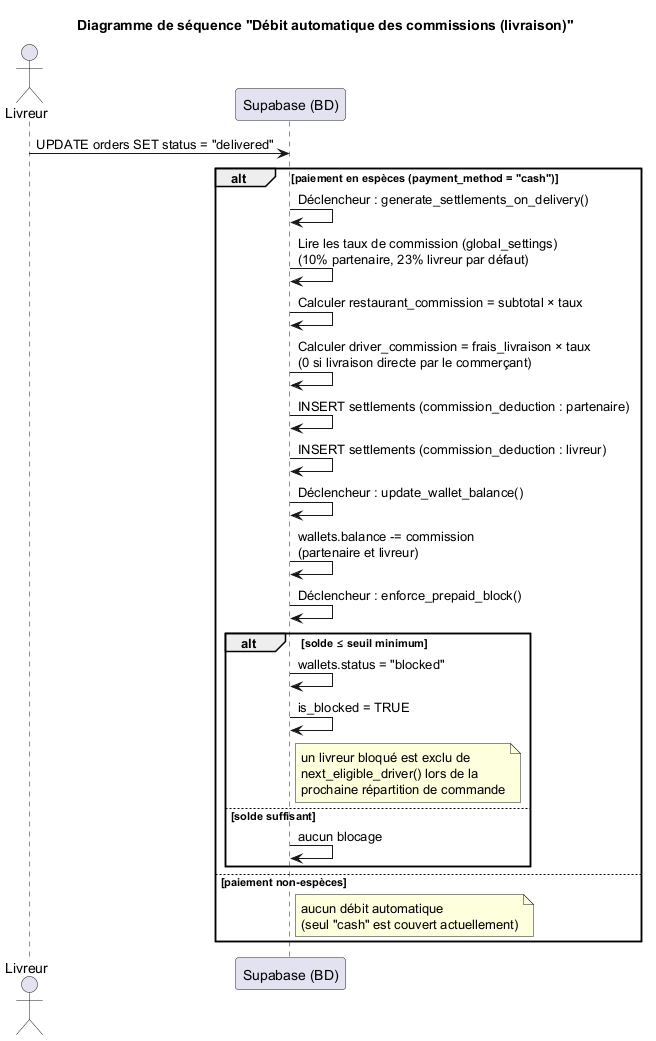
\includegraphics[width=\textwidth]{diagramme_sequence_commission_livraison.png}
\caption{Diagramme de séquence — Débit automatique des commissions}
\label{fig:sequence_commission_livraison}
\end{figure}

Ce mécanisme illustre un choix de conception délibéré~: faire reposer la santé financière du système sur des règles automatiques plutôt que sur une vérification manuelle par l'administrateur, quitte à devoir affiner ces règles au fil du temps, comme le montre l'écart encore présent entre les paiements en espèces et les autres modes de paiement.

\subsection{Envoi d'un colis}

Ce diagramme décrit le parcours suivi par un client lorsqu'il envoie un colis à une autre personne, sans commerçant impliqué, en complément de la description textuelle donnée à la section~2.4.6.

Le client renseigne l'adresse de récupération via sa position GPS, puis l'adresse de dépôt, les numéros de téléphone de l'expéditeur et du destinataire, ainsi qu'une description du colis. L'application calcule alors automatiquement le prix estimé, sur la base d'un tarif fixe majoré d'un montant par kilomètre au-delà d'une distance de base. Le client peut aussi joindre une photo du colis.

Une fois l'envoi confirmé, une commande de type colis est créée directement avec un statut prêt, sans étape de préparation, puisqu'aucun partenaire n'est impliqué. Contrairement aux commandes classiques, ce type de commande n'est poussé vers aucun livreur en particulier~: elle apparaît dans la liste des commandes disponibles, et c'est un livreur qui choisit de l'accepter lui-même, de manière atomique, pour éviter qu'elle soit attribuée à deux livreurs en même temps.

\begin{figure}[H]
\centering
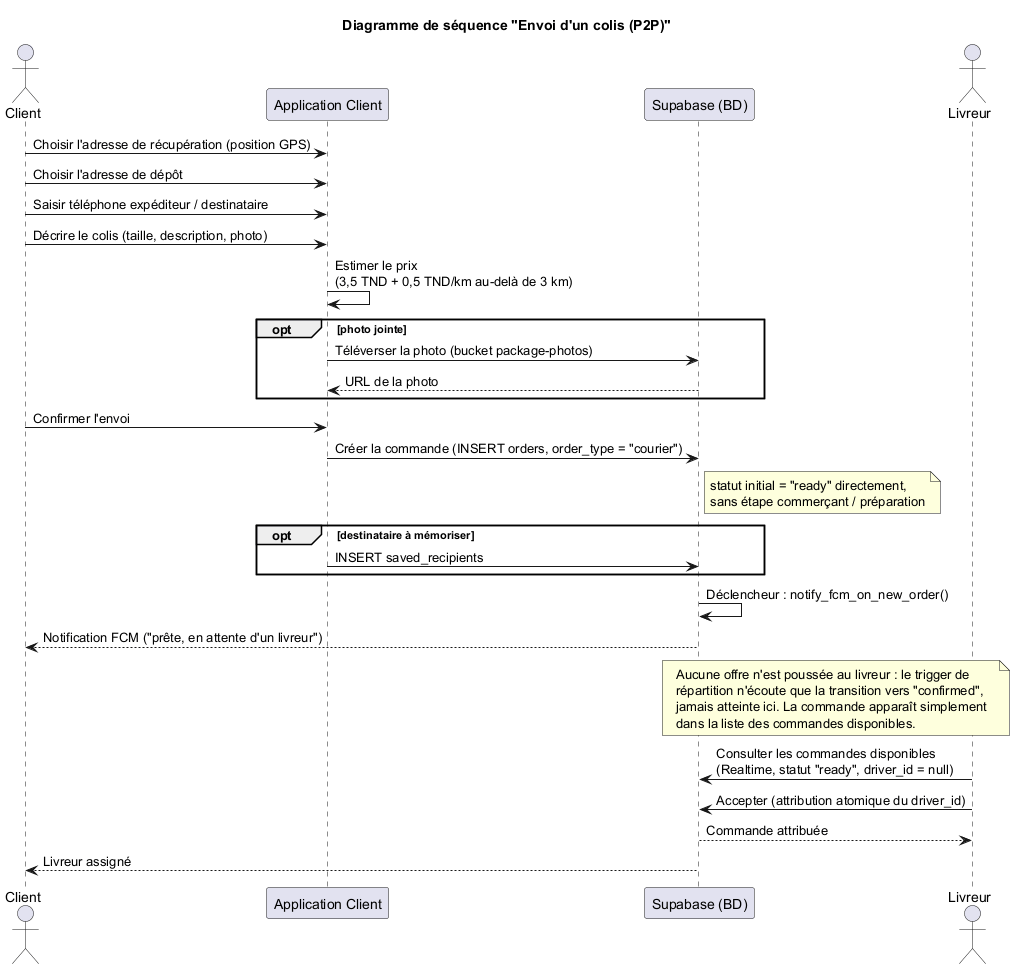
\includegraphics[width=\textwidth]{diagramme_sequence_envoi_colis.png}
\caption{Diagramme de séquence — Envoi d'un colis (P2P)}
\label{fig:sequence_envoi_colis}
\end{figure}

Ce diagramme met en évidence la principale différence entre une commande classique et un envoi de colis~: dans le premier cas, c'est le système qui pousse activement l'offre vers un livreur précis~; dans le second, c'est le livreur qui va chercher l'offre. Ce choix a été fait parce qu'un envoi de colis, contrairement à une commande de repas, n'a pas de contrainte de fraîcheur qui imposerait une attribution immédiate.

\section{Conception des interfaces}

La conception des interfaces des trois applications mobiles a suivi quelques principes simples, appliqués de façon cohérente d'une application à l'autre. Chaque application reprend la même structure de navigation~: une barre de navigation basse avec un nombre réduit d'onglets, adaptée au fait qu'elle est utilisée à une seule main sur un téléphone. Les listes de commerces, de produits ou de commandes sont présentées sous forme de cartes, avec une image, un titre et une information clé (prix, statut, distance), pour permettre un survol rapide de l'information avant d'entrer dans le détail d'un élément.

Les trois applications mobiles utilisent les composants standards fournis par Flutter, ce qui garantit un comportement familier pour l'utilisateur (retour arrière, défilement, champs de saisie) sans avoir à redévelopper ces mécanismes. Le tableau de bord administrateur suit une logique différente, plus proche des standards du web~: menus latéraux, tableaux de données triables, et graphiques pour les indicateurs financiers, puisqu'il est destiné à un usage prolongé depuis un ordinateur plutôt qu'à une consultation rapide depuis un téléphone.

Le texte de l'interface est entièrement en français, ce qui correspond à la langue principale des utilisateurs visés par la phase pilote à Kairouan, avec quelques exceptions ponctuelles côté administrateur héritées des bibliothèques utilisées.

\section{Conclusion}

Ce chapitre a présenté l'analyse et la conception de la plateforme Amana~: les fonctionnalités principales, le diagramme de cas d'utilisation et ses six scénarios détaillés, l'architecture générale du système, le diagramme de classes et les diagrammes de séquence associés. Cette étape de conception a permis de clarifier, avant même d'écrire le code, la façon dont les quatre applications allaient s'articuler autour d'un backend commun. Le chapitre suivant décrit la réalisation technique de cette conception.

%************CHAP3***********
\chapter{Réalisation technique}

\section{Introduction}

Le chapitre précédent a défini l'architecture générale et la structure des données de la plateforme Amana. Ce troisième chapitre explique comment cette conception a été concrètement construite~: les technologies utilisées, l'organisation du code, le fonctionnement du back-end, la sécurité de l'application, l'intégration de l'intelligence artificielle et la gestion des paiements.

\section{Environnement de développement}

Le développement a été fait avec Visual Studio Code et Android Studio, en utilisant le SDK Flutter (version 3.0 ou plus récente) et le langage Dart (version 3.0). Le tableau de bord Administrateur a été développé séparément, toujours avec Visual Studio Code, mais avec Next.js et TypeScript plutôt qu'avec Flutter.

\section{Technologies utilisées}

\subsection{Flutter et Dart}

Les trois applications mobiles (Client, Livreur, Partenaire) sont écrites en Dart avec le framework Flutter~\cite{flutter_docs,dart_docs}. Ce choix permet de maintenir une seule base de code pour Android et pour iOS, avec la même apparence sur les deux systèmes, plutôt que de développer deux applications natives distinctes. Il permet aussi de réutiliser une partie du code entre les trois applications, puisqu'elles partagent des besoins communs~: authentification, affichage d'une carte, gestion d'un panier ou d'un portefeuille.

\subsection{Next.js et TypeScript}

Le tableau de bord Administrateur suit une logique différente~: ce n'est pas une application mobile, mais une application web construite avec Next.js~\cite{nextjs_docs}, un framework basé sur React~\cite{react_docs}, écrite en TypeScript et mise en forme avec Tailwind CSS. Ce choix est cohérent avec son usage~: un administrateur travaille depuis un ordinateur, pas depuis un téléphone, ce qui rend une interface web plus adaptée qu'une application mobile.

\subsection{Supabase et PostgreSQL}

Supabase~\cite{supabase_docs} a été utilisé comme solution back-end pour les quatre applications. Cette plateforme regroupe, en un seul endroit, une base de données PostgreSQL~\cite{postgresql_docs} (version 17.6 sur ce projet), un système d'authentification, un mécanisme de mise à jour en temps réel (Realtime), un espace de stockage pour les fichiers (photos de plats, photos de colis, logos), et un environnement pour exécuter des fonctions côté serveur (Edge Functions). Ces fonctions serveur servent à la fois aux deux fonctionnalités d'intelligence artificielle présentées à la section~\ref{sec:ia}, à l'envoi des notifications, et à la répartition des commandes entre les livreurs.

\subsection{Firebase Cloud Messaging}

Firebase Cloud Messaging (FCM)~\cite{fcm_docs} est le service utilisé pour envoyer les notifications push sur les quatre applications~: confirmation d'une commande côté client, nouvelle offre de livraison côté livreur, nouvelle commande côté partenaire, ou alerte de sécurité côté administrateur. Les notifications sont déclenchées côté serveur, depuis les Edge Functions Supabase, à chaque changement de statut pertinent dans la base de données, plutôt que d'être envoyées directement par les applications mobiles.

\subsection{Mapbox et géolocalisation}

Mapbox~\cite{mapbox_docs} fournit l'affichage des cartes et le calcul d'itinéraire dans l'application Client et l'application Livreur. Côté livreur, la position GPS de l'appareil est envoyée au serveur à chaque déplacement d'environ 30 mètres, grâce à un flux de position filtré par distance (\texttt{distanceFilter}) plutôt qu'à un envoi périodique par minuterie~: cela évite d'envoyer des positions inutiles lorsque le livreur est à l'arrêt, tout en gardant un suivi précis pendant un déplacement.

\section{Organisation du code}

\subsection{Organisation des applications mobiles}

Les trois applications Flutter suivent la même organisation de code, pour rester cohérentes entre elles. Chaque fonctionnalité (commandes, profil, panier, etc.) est rangée dans son propre dossier, séparé en trois parties~:

\begin{itemize}
    \item un dossier \texttt{data}, qui contient les modèles de données et un \emph{repository} — une classe qui centralise tous les échanges avec Supabase pour cette fonctionnalité~;
    \item un dossier \texttt{providers}, qui contient la logique métier et l'état de l'application~;
    \item un dossier \texttt{presentation}, qui contient les écrans et les widgets, qui affichent simplement les données préparées par les providers.
\end{itemize}

Ce découpage reprend directement le patron MVVM présenté au chapitre~2~: \texttt{data} correspond au \textit{Model}, \texttt{presentation} à la \textit{View}, et \texttt{providers} au \textit{ViewModel}. Il évite de mélanger l'affichage et la logique, sans ajouter de couche supplémentaire~: il n'existe pas de classe \textit{ViewModel} séparée dans le projet, c'est directement le \textit{provider} qui joue ce rôle.

\subsection{Gestion de l'état avec Riverpod}

La logique métier et l'état de chaque écran sont gérés avec Riverpod~\cite{riverpod_docs}, une bibliothèque de gestion d'état pour Flutter. Un \textit{provider} Riverpod récupère les données depuis le \textit{repository} du dossier \texttt{data}, les transforme si nécessaire, puis expose un état que l'écran peut observer. Lorsque cet état change — une nouvelle position GPS reçue, un article ajouté au panier, une commande dont le statut vient d'être mis à jour — l'écran concerné se redessine automatiquement, sans que le développeur ait à gérer manuellement cette mise à jour. Ce choix garde le code simple à comprendre, tout en restant assez organisé pour qu'un développeur retrouve facilement ses repères d'une application à l'autre.

\subsection{Organisation de l'application web}

Le tableau de bord Administrateur, construit avec Next.js, n'utilise pas Riverpod puisqu'il n'est pas développé avec Flutter~: il gère son état avec les outils habituels de React. Le code est organisé selon les conventions de Next.js~: le dossier \texttt{app/dashboard/} contient les pages et les composants d'affichage, organisés par domaine fonctionnel (commandes, livreurs, restaurants, finances, etc., voir tableau~\ref{tab:pages_admin} au chapitre~2), et le dossier \texttt{app/api/} contient les routes API qui font le lien avec Supabase. Cette séparation entre pages et routes API correspond directement au découpage Vue / Contrôleur du patron MVC décrit au chapitre~2.

\section{Implémentation du back-end}

\subsection{Authentification des utilisateurs}

L'authentification repose sur Supabase Auth, avec deux méthodes disponibles~: un compte classique par e-mail et mot de passe, ou une connexion directe via Google. Dans les deux cas, une fois le compte créé côté Supabase Auth, un déclencheur SQL insère automatiquement une ligne correspondante dans la table des profils de l'application, pour que chaque utilisateur dispose d'un profil applicatif dès sa première connexion. Un numéro de téléphone est ensuite demandé s'il n'est pas déjà renseigné, sans passer par une vérification par SMS, comme détaillé dans le diagramme de séquence du chapitre~2.

\subsection{Gestion des données}

Chaque table de la base de données PostgreSQL est protégée par des règles de sécurité au niveau des lignes (\textit{Row Level Security}, RLS). Ces règles définissent, pour chaque rôle d'utilisateur, quelles lignes il a le droit de lire ou de modifier~: un client ne peut voir que ses propres commandes et adresses, un livreur ne voit que les commandes qui lui sont proposées ou attribuées, un partenaire ne voit que son propre catalogue et ses propres commandes. Cette approche centralise la logique de séparation des données directement dans la base, plutôt que de la répéter dans chacune des quatre applications.

\subsection{Gestion des commandes}

Une commande passe par une suite de statuts, au nombre de huit dans l'état actuel du système~: \textit{en attente}, \textit{confirmée}, \textit{en préparation}, \textit{prête}, \textit{récupérée}, \textit{en livraison}, \textit{livrée} et \textit{annulée}. Ce nombre est passé de cinq à huit au cours du projet, comme mentionné au chapitre~1, pour mieux représenter les étapes réelles observées lors des tests. La création d'une commande se fait en une seule écriture en base, au moment de la confirmation finale par le client~; les étapes précédentes (panier, choix de l'adresse, choix du paiement) restent locales à l'application.

\subsection{Gestion des livraisons}

Lorsqu'une commande passe au statut confirmée, le serveur cherche automatiquement un livreur disponible dans un rayon d'environ 7~km autour du point de collecte, et lui envoie une offre avec un délai d'environ 30~secondes pour l'accepter ou la refuser. Si le livreur ne répond pas dans ce délai, ou refuse explicitement, l'offre est retirée et proposée au livreur disponible suivant dans le même rayon~: c'est le mécanisme de \textit{dispatch en cascade} déjà évoqué au chapitre~2. Ce mécanisme est mis en œuvre par une fonction stockée côté base de données, appelée à la fois lors de la confirmation de la commande et lors de l'expiration d'une offre non traitée. Pendant la livraison, la position GPS du livreur est mise à jour dans la base à chaque déplacement d'environ 30~mètres, ce qui permet au client de suivre sa commande en direct, comme décrit au chapitre~2.

\subsection{Notifications en temps réel}

Deux mécanismes complémentaires assurent la circulation de l'information en temps réel. Les notifications push, envoyées via Firebase Cloud Messaging, informent un utilisateur même lorsque l'application est fermée ou en arrière-plan~: nouvelle offre de livraison, changement de statut d'une commande, nouvelle commande reçue par un partenaire. Supabase Realtime, de son côté, met à jour automatiquement les écrans déjà ouverts, comme la position du livreur sur la carte du client, ou la liste des commandes du tableau de bord Administrateur, sans que l'utilisateur ait besoin de rafraîchir la page ou l'écran manuellement.

\section{Sécurité de l'application}

\subsection{Gestion des rôles}

Chaque utilisateur de la plateforme appartient à un rôle précis~: client, livreur, partenaire ou administrateur. Ce rôle détermine à la fois l'application qu'il peut utiliser et les données auxquelles il a accès. Côté base de données, ce contrôle est appliqué par les règles RLS décrites plus haut. Côté tableau de bord web, chaque route API vérifie explicitement que l'appelant est bien un administrateur authentifié, grâce à la fonction \texttt{requireAdmin()}, avant de traiter la moindre requête sensible.

\subsection{Protection des données}

Toutes les communications entre les applications et le backend passent en HTTPS. Les appels aux fonctions serveur Supabase (Edge Functions) sont vérifiés avant même l'exécution du code applicatif, grâce à un jeton d'authentification (JWT) associé à l'utilisateur connecté~: un appel non authentifié est rejeté automatiquement par la plateforme. Un middleware Next.js redirige par ailleurs tout utilisateur non authentifié qui tenterait d'accéder directement à une page du tableau de bord Administrateur vers l'écran de connexion.

\subsection{Gestion des clés d'accès}

Les clés sensibles — accès aux fournisseurs d'intelligence artificielle, clé \texttt{service\_role} de Supabase qui donne un accès complet à la base de données — sont stockées comme des secrets côté serveur et ne sont jamais incluses dans le code des applications mobiles installées sur les téléphones. Ce choix corrige une pratique risquée présente dans une version antérieure du projet, où une clé était directement intégrée à l'application mobile~: une application installée pouvant être analysée pour en extraire son contenu, une telle clé aurait pu être récupérée par n'importe qui. Le tableau de bord Administrateur utilise la clé \texttt{service\_role} uniquement dans ses routes API, côté serveur, jamais transmise au navigateur.

\section{Intégration des fonctionnalités d'intelligence artificielle}
\label{sec:ia}

Deux fonctionnalités de la plateforme Amana font appel à l'intelligence artificielle~: un assistant conversationnel et un moteur de recherche intelligente. Contrairement au reste de l'application, ces deux fonctionnalités n'utilisent pas uniquement la base de données interne~: elles envoient des requêtes, par le réseau, à des modèles de langage hébergés chez des fournisseurs externes.

Héberger son propre modèle de langage demande une puissance de calcul coûteuse, hors de portée d'un projet de ce type. Comme la plupart des applications actuelles, Amana envoie donc une simple requête HTTPS, au format JSON, à un modèle hébergé ailleurs. La figure~\ref{fig:archi-ia} montre l'organisation retenue, commune aux deux fonctionnalités~: l'application mobile récupère la demande de l'utilisateur (texte, photo ou message vocal), une fonction Edge Supabase sert d'intermédiaire de confiance, et les fournisseurs de modèles de langage sont contactés depuis cette fonction serveur plutôt que directement depuis le téléphone.

\begin{figure}[H]
    \centering
    \fbox{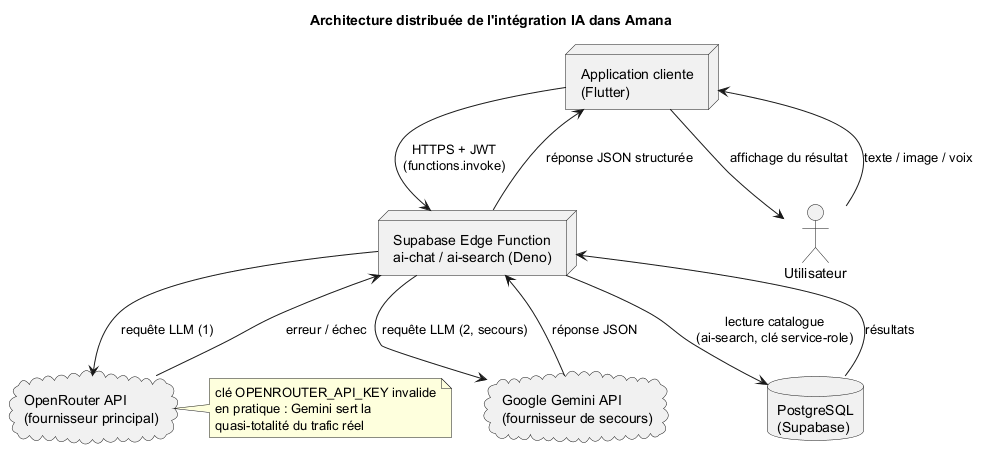
\includegraphics[width=\textwidth,keepaspectratio]{diagramme_architecture_ia.png}}
    \caption{Architecture distribuée de l'intégration de l'IA dans Amana}
    \label{fig:archi-ia}
\end{figure}

Ce passage par un serveur intermédiaire répond à un besoin de sécurité déjà évoqué à la section~3.6.3~: dans une première version du projet, l'application appelait directement le fournisseur d'IA depuis le téléphone, avec la clé d'accès stockée dans l'application elle-même, ce qui l'exposait à une extraction. En déplaçant cet appel vers le serveur, cette clé n'est plus jamais présente sur le téléphone de l'utilisateur.

\subsection{Assistant conversationnel}

L'assistant conversationnel, appelé « Amana Assistant », est accessible depuis un bouton flottant sur l'écran d'accueil de l'application Client. Le client peut y écrire un message, joindre une photo d'un plat, ou dicter son message grâce à la reconnaissance vocale du téléphone, qui fonctionne directement sur l'appareil sans passer par le réseau. La langue de réponse (français, arabe, dialecte tunisien ou anglais) est détectée dès le premier message et gardée pendant toute la conversation.

Le comportement de l'assistant est fixé par une instruction envoyée à chaque appel, qui lui donne un double rôle de conseiller nutritionnel et de moteur de recherche de plats, avec une correspondance entre des objectifs exprimés simplement (régime, sport, diabète, cholestérol, ramadan) et des mots-clés de recherche. L'assistant répond toujours dans un format fixe~: un objet JSON contenant un message à afficher et une intention (recherche d'un plat, recherche à l'épicerie, envoi de colis, simple salutation). Ce format permet de garder le résultat imprévisible du modèle de langage à un seul endroit du système~: le reste de l'application continue de travailler avec des données classiques et prévisibles. L'historique de la conversation n'est pas gardé côté serveur~: c'est l'application, sur le téléphone, qui le conserve et le renvoie en entier à chaque nouveau message, ce qui simplifie la bascule entre fournisseurs décrite ci-dessous, au prix de perdre la conversation à la fermeture de l'application.

\subsection{Recherche intelligente}

La recherche intelligente retrouve des articles du catalogue à partir d'un texte libre ou d'une photo d'un plat. Il est important de préciser qu'elle \textbf{n'utilise pas de recherche vectorielle sémantique}~: il n'existe ni extension \texttt{pgvector}, ni colonne d'embedding dans la base de données. Il s'agit d'une combinaison plus simple, moins coûteuse à construire et à maintenir~: un modèle de langage qui analyse la demande, puis une requête classique sur la base relationnelle.

Pour une requête en texte, le traitement se fait en trois étapes~: un premier appel au modèle transforme le texte libre en critères précis (catégorie, prix, épicé ou non, végétarien ou non, mot-clé)~; ces critères interrogent la table des articles avec un relâchement progressif — si aucun résultat exact n'est trouvé, le système retire d'abord les critères les moins importants, puis la catégorie, puis le prix, jusqu'à trouver des résultats, présentés alors comme une suggestion~; enfin, un second appel classe les résultats du plus au moins pertinent, avec un tri par prix croissant comme solution de repli si cet appel échoue. Le mode photo suit une logique proche~: un modèle capable d'analyser les images identifie d'abord le plat, puis les mots-clés obtenus servent à la même requête et au même classement. Contrairement à l'assistant conversationnel, cette fonction accède directement à la base de données avec la clé \texttt{service-role}, ce qui lui permet de préparer les résultats entièrement côté serveur.

\subsection{Communication avec les services externes}

L'application et la fonction serveur communiquent en HTTPS, au format JSON, en mode question/réponse classique — sans flux continu~: la réponse n'est envoyée qu'une fois que le modèle a fini de la générer entièrement. Avant même d'exécuter le code de la fonction, Supabase vérifie que l'appelant est bien connecté, grâce à un jeton JWT~: les deux fonctions exigent cette vérification (\texttt{verify\_jwt = true}), et un appel non authentifié est rejeté avant même d'atteindre le code applicatif. Côté application, l'appel à l'assistant conversationnel a une limite de temps de 60~secondes, plus large que d'habitude, pour laisser le temps de traiter un message accompagné d'une photo.

Plusieurs fournisseurs proposent ce type de service~: Google, OpenAI, Anthropic, Meta, Mistral, entre autres. Certaines plateformes, comme OpenRouter, servent d'intermédiaire en redirigeant la requête vers l'un ou l'autre de ces fournisseurs selon le modèle demandé. Amana utilise ce type de plateforme comme fournisseur principal, avec un second fournisseur en secours si le premier ne répond pas.

\subsection{Gestion des erreurs et des fournisseurs de secours}

Dépendre d'un service externe, accessible uniquement par le réseau, revient à accepter le risque que ce service soit indisponible. Pour limiter ce risque, la fonction serveur essaie d'abord d'appeler le fournisseur principal, OpenRouter. Si cet appel échoue — réponse d'erreur, contenu mal formé ou réponse vide — la fonction bascule aussitôt vers un second appel, cette fois directement vers l'API de Google Gemini, avec la même requête adaptée à son format.

Ce mécanisme n'est pas resté théorique~: la clé d'accès utilisée pour OpenRouter s'est révélée invalide, et chaque appel vers ce fournisseur échoue avec une erreur d'authentification. En pratique, la quasi-totalité des demandes réelles des deux fonctionnalités passe donc aujourd'hui par le chemin de secours, Gemini. Ce qui devait être une simple sécurité est ainsi devenu, dans les faits, le chemin qui fait réellement fonctionner ces deux fonctionnalités. Cette bascule reste invisible pour l'utilisateur~: comme chaque requête contient déjà tout l'historique nécessaire, changer de fournisseur au milieu d'une conversation ne fait perdre aucune information.

Cette intégration reste perfectible, ce qui est cohérent avec le cadre d'un projet de fin d'études~: il n'y a pas de limite de nombre d'appels par utilisateur, pas de mise en cache des réponses, pas de réponse progressive (\textit{streaming}), et la recherche reste basée sur une correspondance de mots-clés plutôt que sur une vraie recherche sémantique. Ces limites sont reprises comme pistes d'évolution au chapitre~5.

\section{Gestion des paiements, commissions et récompenses}

Chaque livreur et chaque partenaire dispose d'un portefeuille électronique dans lequel sont enregistrés les gains et les commissions prélevées par la plateforme. Lorsqu'une commande réglée en espèces est livrée, une commission de dix pour cent est prélevée sur le montant des articles pour le partenaire, et une commission de vingt-trois pour cent est prélevée sur les frais de livraison pour le livreur~; ces taux sont configurables depuis les paramètres de la plateforme, avec ces valeurs comme défaut. Le solde de chaque portefeuille est mis à jour automatiquement à ce moment-là.

Le modèle retenu est un modèle prépayé~: si le solde d'un livreur devient négatif ou nul, son compte est automatiquement bloqué et il n'est plus proposé lors de la répartition des commandes suivantes, jusqu'à ce qu'il recharge son portefeuille. Un avertissement s'affiche déjà lorsque le solde descend entre deux et quatre dinars, avant d'atteindre ce seuil de blocage. Ce mécanisme protège la plateforme contre un livreur qui accumulerait des commissions dues sans jamais les régler.

En complément, un programme de fidélité permet au client de cumuler des points à chaque commande, consultables et échangeables depuis l'application Client, et suivis côté administrateur pour le règlement des primes correspondantes.

\section{Conclusion}

Ce chapitre a détaillé la réalisation technique de la plateforme Amana~: les technologies retenues pour chacune des quatre applications, l'organisation du code autour des patrons MVVM et MVC, le fonctionnement du back-end pour l'authentification, les commandes et les livraisons, la sécurité des données et des clés d'accès, l'intégration des deux fonctionnalités d'intelligence artificielle, ainsi que la gestion des paiements et des commissions. Le chapitre suivant montre le résultat concret de ce travail, à travers une présentation des quatre applications et de leurs interfaces.

%************CHAP4***********
\chapter{Présentation des applications et des interfaces}

\section{Introduction}

Les trois chapitres précédents ont présenté les besoins, la conception et la réalisation technique de la plateforme Amana. Ce quatrième chapitre montre le résultat concret de ce travail~: à quoi ressemble chacune des quatre applications, et comment un utilisateur les utilise au quotidien. Chaque section reprend l'un des quatre acteurs identifiés au chapitre~1, en détaillant ses écrans principaux.

\section{Application client}

L'application Client est destinée au grand public~: toute personne disposant d'un smartphone Android ou iOS et souhaitant commander un repas, faire ses courses, envoyer un colis ou faire payer une facture.

\subsection{Authentification}

L'écran d'authentification, présenté à la figure~\ref{fig:client_auth}, propose au client de créer un compte ou de se connecter, avec la possibilité de passer directement par un compte Google pour éviter la saisie d'un mot de passe.

\begin{figure}[H]
    \centering
    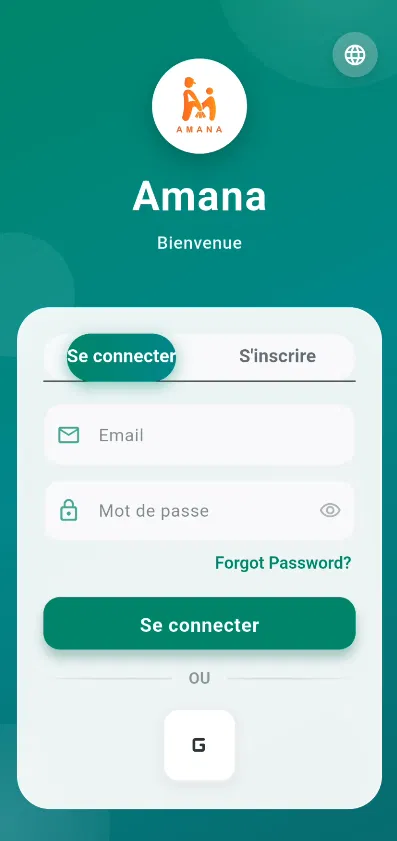
\includegraphics[height=0.5\textheight,keepaspectratio]{client_auth.png}
    \caption{Écran d'authentification — application Client}
    \label{fig:client_auth}
\end{figure}

Cet écran correspond directement au cas d'utilisation décrit à la section~2.4.1~: les trois chemins possibles (création de compte, connexion classique, connexion Google) y sont accessibles depuis les mêmes boutons.

\subsection{Page d'accueil}

Une fois connecté, le client arrive sur l'écran d'accueil (figure~\ref{fig:client_accueil}), qui donne accès aux quatre services présentés au chapitre~1~: livraison de repas, supermarché, colis et facture, ainsi qu'à une liste de restaurants populaires et à une barre de recherche.

\begin{figure}[H]
    \centering
    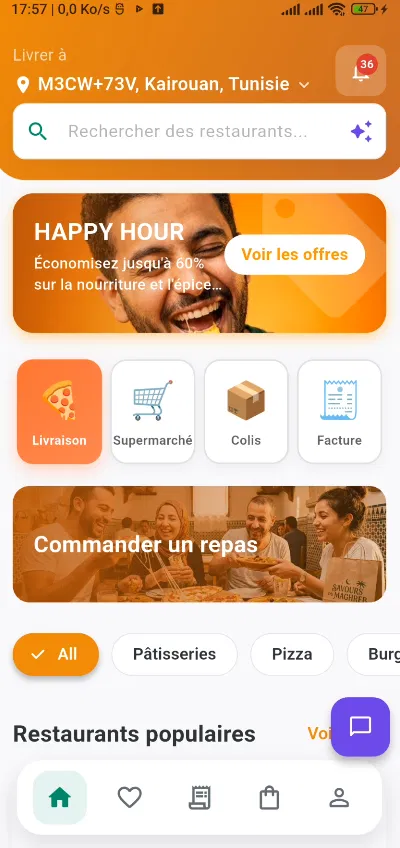
\includegraphics[height=0.5\textheight,keepaspectratio]{client_accueil.png}
    \caption{Écran d'accueil — application Client}
    \label{fig:client_accueil}
\end{figure}

Le choix de regrouper les quatre services sur un seul écran d'accueil, plutôt que de les répartir dans un menu, reflète directement la solution proposée au chapitre~1~: donner accès à plusieurs services depuis un seul point d'entrée.

\subsection{Consultation des restaurants et des produits}

Depuis la liste des restaurants, le client accède au détail d'un commerce et à son menu (figure~\ref{fig:client_restaurant}), avec un système de catégories pour filtrer les articles proposés.

\begin{figure}[H]
    \centering
    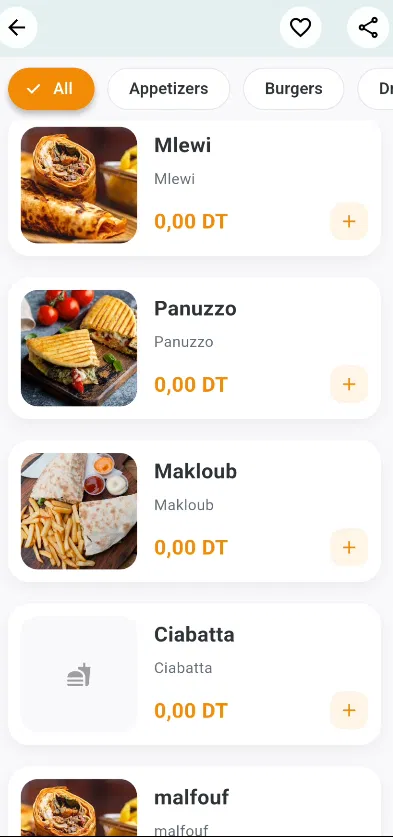
\includegraphics[height=0.5\textheight,keepaspectratio]{client_restaurant_detail.png}
    \caption{Détail d'un restaurant et de son menu — application Client}
    \label{fig:client_restaurant}
\end{figure}

Cet écran illustre le cas d'utilisation « ajouter des produits au panier » décrit à la section~2.4.2~: chaque article de la liste dispose d'un bouton d'ajout direct, sans passer par un écran de détail intermédiaire pour les articles simples.

\subsection{Panier et validation de la commande}

Le panier permet au client de vérifier les articles sélectionnés, de modifier les quantités, puis de choisir une adresse et un mode de paiement avant de valider sa commande, comme décrit dans le raffinement de la section~2.4.2.

% TODO : ajouter la capture d'écran du panier (liste des articles sélectionnés, quantités, sous-total)
% \begin{figure}[H]
%     \centering
%     \includegraphics[height=0.5\textheight,keepaspectratio]{client_panier.png}
%     \caption{Panier — application Client}
%     \label{fig:client_panier}
% \end{figure}

% TODO : ajouter la capture d'écran de l'écran de validation de commande (choix adresse + paiement)
% \begin{figure}[H]
%     \centering
%     \includegraphics[height=0.5\textheight,keepaspectratio]{client_checkout.png}
%     \caption{Validation de la commande — application Client}
%     \label{fig:client_checkout}
% \end{figure}

Ces deux écrans concentrent l'essentiel des interactions du client avant la confirmation finale, qui déclenche l'écriture en base décrite dans le diagramme de séquence de la section~2.7.2.

\subsection{Suivi de la livraison}

Une fois la commande confirmée, le client peut suivre sa progression en direct (figure~\ref{fig:client_suivi}), avec la position du livreur affichée sur une carte et un indicateur de l'étape en cours parmi les huit statuts possibles.

\begin{figure}[H]
    \centering
    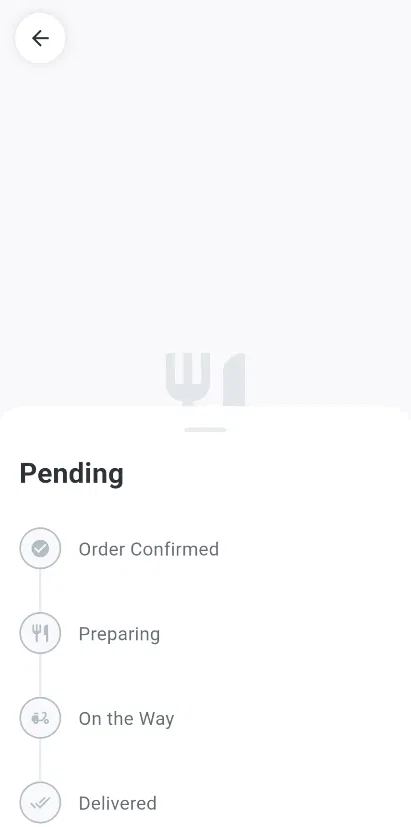
\includegraphics[height=0.5\textheight,keepaspectratio]{client_suivi_commande.png}
    \caption{Suivi de la commande en temps réel — application Client}
    \label{fig:client_suivi}
\end{figure}

Cet écran illustre concrètement le raffinement « suivre la commande » décrit à la section~2.4.3~: on y retrouve l'indicateur de statut, la carte avec le marqueur du livreur, et l'accès à l'annulation tant que la commande n'a pas été prise en charge.

\subsection{Assistant conversationnel et recherche intelligente}

Enfin, le client dispose de deux outils basés sur l'intelligence artificielle, détaillés au chapitre~3~: un assistant conversationnel (figure~\ref{fig:client_assistant}) et une recherche intelligente par texte ou par photo (figure~\ref{fig:client_recherche}).

\begin{figure}[H]
    \centering
    
\includegraphics[height=0.5\textheight,keepaspectratio]{client_assistant_ia.png}
    \caption{Assistant conversationnel « Amana Assistant » — application Client}
    \label{fig:client_assistant}
\end{figure}

\begin{figure}[H]
    \centering
    
\includegraphics[height=0.5\textheight,keepaspectratio]{client_recherche_ia.png}
    \caption{Recherche intelligente par texte ou par photo — application Client}
    \label{fig:client_recherche}
\end{figure}

Ces deux écrans montrent les exemples de suggestions proposées à l'utilisateur (« Une pizza pas chère », « Un malfouf à moins de 12 dinars ») ainsi que la possibilité d'envoyer directement une photo d'un plat, deux façons différentes d'arriver au même résultat~: une liste d'articles pertinents.

\section{Application livreur}

Cette application est destinée aux livreurs partenaires de la plateforme, équipés d'un smartphone avec GPS et connexion internet.

\subsection{Authentification}

% TODO : ajouter la capture d'écran de l'authentification côté livreur
% \begin{figure}[H]
%     \centering
%     \includegraphics[height=0.5\textheight,keepaspectratio]{livreur_auth.png}
%     \caption{Écran d'authentification — application Livreur}
%     \label{fig:livreur_auth}
% \end{figure}

L'écran d'authentification du livreur reprend le même principe que celui du client, décrit à la section~4.2.1, avec les mêmes chemins de connexion.

\subsection{Gestion de la disponibilité}

% TODO : ajouter la capture d'écran de l'écran d'accueil livreur (bouton disponible / indisponible)
% \begin{figure}[H]
%     \centering
%     \includegraphics[height=0.5\textheight,keepaspectratio]{livreur_accueil.png}
%     \caption{Tableau de bord et statut en ligne — application Livreur}
%     \label{fig:livreur_accueil}
% \end{figure}

Depuis l'écran d'accueil, le livreur se déclare disponible ou non. Ce statut détermine s'il peut recevoir des offres de commande~: un livreur indisponible n'est jamais sollicité par le mécanisme de dispatch décrit au chapitre~3.

\subsection{Consultation des commandes disponibles}

% TODO : ajouter la capture d'écran de la liste des commandes disponibles
% \begin{figure}[H]
%     \centering
%     \includegraphics[height=0.5\textheight,keepaspectratio]{livreur_commandes_disponibles.png}
%     \caption{Liste des commandes disponibles — application Livreur}
%     \label{fig:livreur_commandes}
% \end{figure}

Quand il est disponible, le livreur voit la liste des commandes qui lui sont proposées dans son rayon d'action, avec le commerçant concerné, l'adresse du client et le montant de la course.

\subsection{Acceptation et refus d'une commande}

% TODO : ajouter la capture d'écran de l'écran d'offre de commande avec le compte à rebours
% \begin{figure}[H]
%     \centering
%     \includegraphics[height=0.5\textheight,keepaspectratio]{livreur_offre_commande.png}
%     \caption{Offre de commande à accepter ou refuser — application Livreur}
%     \label{fig:livreur_offre}
% \end{figure}

Pour chaque offre, le livreur dispose d'environ 30~secondes pour l'accepter ou la refuser, comme décrit à la section~3.5.4. En cas de non-réponse ou de refus, l'offre est automatiquement proposée au livreur disponible suivant.

\subsection{Suivi de la livraison}

% TODO : ajouter la capture d'écran de l'écran de suivi de livraison en cours (carte + itinéraire)
% \begin{figure}[H]
%     \centering
%     \includegraphics[height=0.5\textheight,keepaspectratio]{livreur_suivi_livraison.png}
%     \caption{Suivi de la livraison en cours — application Livreur}
%     \label{fig:livreur_suivi}
% \end{figure}

Une fois la commande acceptée, l'application affiche l'itinéraire à suivre sur une carte Mapbox et permet au livreur de mettre à jour le statut de la livraison étape par étape, jusqu'à la remise finale au client.

\subsection{Revenus et portefeuille}

% TODO : ajouter la capture d'écran de l'écran de revenus et de portefeuille du livreur
% \begin{figure}[H]
%     \centering
%     \includegraphics[height=0.5\textheight,keepaspectratio]{livreur_revenus.png}
%     \caption{Revenus et portefeuille — application Livreur}
%     \label{fig:livreur_revenus}
% \end{figure}

Le livreur peut consulter à tout moment son solde de portefeuille et l'historique de ses gains, alimenté automatiquement à chaque livraison réglée en espèces, comme décrit à la section~3.8.

\section{Application partenaire}

Cette application est destinée aux restaurateurs, aux responsables de supermarchés et, plus largement, à tous les commerçants partenaires qui gèrent leurs commandes via la plateforme.

\subsection{Gestion du catalogue}

% TODO : ajouter la capture d'écran du catalogue de produits du partenaire
% \begin{figure}[H]
%     \centering
%     \includegraphics[height=0.5\textheight,keepaspectratio]{partenaire_menu.png}
%     \caption{Catalogue de produits — application Partenaire}
%     \label{fig:partenaire_menu}
% \end{figure}

Le commerçant gère son catalogue de produits ou de plats~: ajout, modification, disponibilité et horaires d'ouverture, avec un affichage organisé par catégorie.

\subsection{Ajout et modification d'un article}

% TODO : ajouter la capture d'écran du formulaire d'ajout / modification d'un article
% \begin{figure}[H]
%     \centering
%     \includegraphics[height=0.5\textheight,keepaspectratio]{partenaire_ajout_article.png}
%     \caption{Ajout / modification d'un article — application Partenaire}
%     \label{fig:partenaire_article}
% \end{figure}

Ce formulaire reprend les informations décrites dans le diagramme de classes du chapitre~2 pour un article~: nom, prix, catégorie et photo, avec une gestion de stock supplémentaire pour les produits de supermarché.

\subsection{Gestion des commandes reçues}

% TODO : ajouter la capture d'écran d'une nouvelle commande entrante (alerte sonore)
% \begin{figure}[H]
%     \centering
%     \includegraphics[height=0.5\textheight,keepaspectratio]{partenaire_commande_entrante.png}
%     \caption{Nouvelle commande entrante — application Partenaire}
%     \label{fig:partenaire_entrante}
% \end{figure}

% TODO : ajouter la capture d'écran de la liste des commandes du partenaire
% \begin{figure}[H]
%     \centering
%     \includegraphics[height=0.5\textheight,keepaspectratio]{partenaire_liste_commandes.png}
%     \caption{Liste des commandes — application Partenaire}
%     \label{fig:partenaire_liste}
% \end{figure}

Le commerçant reçoit les nouvelles commandes en direct, avec une alerte sonore, grâce à Supabase Realtime décrit au chapitre~3. Il peut les accepter ou les refuser, puis suivre leur préparation depuis la liste des commandes en cours.

\subsection{Gestion du plat du jour}

Le partenaire dispose d'un écran dédié pour mettre en avant un plat du jour, selon le mécanisme décrit à la section~2.4.5~: recherche d'un plat existant, puis association ou création, avant validation. Cette fonctionnalité ne dispose pas encore d'une capture d'écran dédiée dans ce rapport~; son fonctionnement est illustré par le raffinement et le diagramme de séquence correspondants au chapitre~2.

\subsection{Statistiques et commissions}

% TODO : ajouter la capture d'écran du portefeuille et des statistiques du partenaire
% \begin{figure}[H]
%     \centering
%     \includegraphics[height=0.5\textheight,keepaspectratio]{partenaire_portefeuille.png}
%     \caption{Portefeuille et commissions — application Partenaire}
%     \label{fig:partenaire_portefeuille}
% \end{figure}

Le commerçant consulte ses statistiques du jour (chiffre d'affaires, nombre de commandes), ainsi que son solde de portefeuille et les commissions prélevées par la plateforme, calculées selon le taux décrit à la section~3.8.

\section{Application administrateur}

Cette application est destinée à l'équipe qui supervise l'ensemble de la plateforme. Contrairement aux trois autres applications, ce n'est pas une application mobile mais un tableau de bord web, pensé pour être utilisé depuis un ordinateur.

\subsection{Tableau de bord}

% TODO : ajouter la capture d'écran de connexion et du tableau de bord principal de l'administrateur
% \begin{figure}[H]
%     \centering
%     \includegraphics[width=0.85\textwidth,keepaspectratio]{admin_login.png}
%     \caption{Écran de connexion — tableau de bord Administrateur}
%     \label{fig:admin_login}
% \end{figure}
% \begin{figure}[H]
%     \centering
%     \includegraphics[width=0.85\textwidth,keepaspectratio]{admin_dashboard.png}
%     \caption{Vue d'ensemble — tableau de bord Administrateur}
%     \label{fig:admin_dashboard}
% \end{figure}

Après une connexion réservée aux comptes administrateurs déjà autorisés, le tableau de bord principal donne une vue d'ensemble de l'activité du jour~: commandes, livreurs en ligne, restaurants actifs, commissions et revenu total, mis à jour en temps réel comme décrit au chapitre~3.

\subsection{Gestion des utilisateurs}

% TODO : ajouter la capture d'écran de la gestion des comptes clients
% \begin{figure}[H]
%     \centering
%     \includegraphics[width=0.85\textwidth,keepaspectratio]{admin_clients.png}
%     \caption{Gestion des clients — tableau de bord Administrateur}
%     \label{fig:admin_clients}
% \end{figure}

Cette section permet de consulter les profils des clients et leur historique de commandes, et d'intervenir sur un compte si nécessaire, dans le respect des règles RLS décrites au chapitre~3.

\subsection{Gestion des restaurants et des commerces}

% TODO : ajouter la capture d'écran de la gestion des restaurants et partenaires
% \begin{figure}[H]
%     \centering
%     \includegraphics[width=0.85\textwidth,keepaspectratio]{admin_restaurants.png}
%     \caption{Gestion des restaurants et partenaires — tableau de bord Administrateur}
%     \label{fig:admin_restaurants}
% \end{figure}

L'administrateur peut ajouter ou modifier un commerce partenaire, gérer ses catégories et sa disponibilité, en complément de ce que le commerçant gère lui-même depuis l'application Partenaire.

\subsection{Gestion des livreurs}

% TODO : ajouter la capture d'écran de la gestion des livreurs (liste + position en direct)
% \begin{figure}[H]
%     \centering
%     \includegraphics[width=0.85\textwidth,keepaspectratio]{admin_livreurs.png}
%     \caption{Gestion des livreurs — tableau de bord Administrateur}
%     \label{fig:admin_livreurs}
% \end{figure}

Cette section liste les livreurs, leur statut en ligne et leur position en direct, et permet de régler manuellement une prime ou de consulter le solde de leur portefeuille.

\subsection{Gestion des commandes}

% TODO : ajouter la capture d'écran de la gestion des commandes (suivi, recherche, annulation)
% \begin{figure}[H]
%     \centering
%     \includegraphics[width=0.85\textwidth,keepaspectratio]{admin_commandes.png}
%     \caption{Gestion des commandes — tableau de bord Administrateur}
%     \label{fig:admin_commandes}
% \end{figure}

L'administrateur peut suivre, rechercher ou annuler une commande, et consulter son historique complet, y compris les commandes de type colis décrites au chapitre~1.

\subsection{Gestion des finances et des commissions}

% TODO : ajouter la capture d'écran de la page des finances (graphiques, export)
% \begin{figure}[H]
%     \centering
%     \includegraphics[width=0.85\textwidth,keepaspectratio]{admin_finances.png}
%     \caption{Finances — tableau de bord Administrateur}
%     \label{fig:admin_finances}
% \end{figure}

Cette page présente les commissions perçues sous forme de graphiques, avec un export possible au format PDF et CSV, pour un suivi financier détaillé de l'activité de la plateforme.

\subsection{Paramètres du système}

% TODO : ajouter la capture d'écran des paramètres du système (taux de commission, codes promo)
% \begin{figure}[H]
%     \centering
%     \includegraphics[width=0.85\textwidth,keepaspectratio]{admin_parametres.png}
%     \caption{Paramètres du système — tableau de bord Administrateur}
%     \label{fig:admin_parametres}
% \end{figure}

C'est depuis cette page que sont configurés les taux de commission par défaut décrits à la section~3.8, ainsi que les codes promotionnels et les autres réglages généraux de la plateforme. Un journal d'activité garde une trace de toutes les actions sensibles effectuées par les administrateurs, comme le blocage d'un compte.

\section{Conclusion}

Ce chapitre a présenté, application par application, le résultat concret de la réalisation~: l'application Client et ses six fonctionnalités principales, l'application Livreur organisée autour du cycle disponibilité / offre / livraison, l'application Partenaire centrée sur la gestion du catalogue et des commandes, et le tableau de bord Administrateur pensé comme un outil de supervision. On retrouve une cohérence forte entre les trois applications mobiles, qui partagent la même base technique et la même organisation de code, présentée au chapitre~3. Le chapitre suivant présente les tests effectués sur ces quatre applications, ainsi que l'état du déploiement et les pistes de maintenance envisagées.

%************CHAP5***********
\chapter{Tests, déploiement et maintenance}

\section{Introduction}

Après avoir présenté la conception, la réalisation et le résultat visible de la plateforme Amana, ce dernier chapitre revient sur la façon dont le système a été vérifié, sur l'état actuel de son déploiement, et sur les pistes envisagées pour la suite. Les tests décrits ici ont été réalisés manuellement, sur des appareils physiques, plutôt qu'à travers une suite de tests automatisés~: ce choix est cohérent avec le calendrier resserré d'un projet de fin d'études, mais il est clairement identifié comme une limite à la section~5.6.

\section{Tests fonctionnels}

\subsection{Test de l'authentification}

Les trois chemins de connexion décrits au chapitre~2 (création de compte, connexion classique, connexion Google) ont été testés manuellement sur des appareils Android réels, en vérifiant à chaque fois qu'un profil est bien créé dans la base de données et que l'écran de saisie du numéro de téléphone n'apparaît que lorsque ce numéro est réellement absent du profil. La figure~\ref{fig:test_auth} montre le résultat attendu de ce test~: une nouvelle ligne de profil correctement créée dans la base de données juste après l'inscription.

% TODO : ajouter la capture d'écran du test d'authentification (ex. ligne de profil créée dans la table Supabase après inscription, ou écran de saisie du numéro de téléphone)
% \begin{figure}[H]
%     \centering
%     \includegraphics[width=0.85\textwidth,keepaspectratio]{test_authentification.png}
%     \caption{Preuve du test d'authentification — profil créé après inscription}
%     \label{fig:test_auth}
% \end{figure}

Ce test confirme que la création du profil applicatif, décrite comme automatique au chapitre~3, se déclenche bien à chaque nouvelle inscription, sans exception observée sur les trois chemins de connexion testés.

\subsection{Test de la création d'une commande}

Le parcours complet — sélection d'articles, personnalisation, choix d'adresse, choix de paiement, confirmation — a été testé de bout en bout, en vérifiant après chaque commande que la ligne correspondante est bien créée dans la base de données, avec le bon statut initial et le bon montant total. La figure~\ref{fig:test_commande} illustre cette vérification, effectuée directement dans l'éditeur de tables de Supabase.

% TODO : ajouter la capture d'écran de la commande créée dans la table "orders" de Supabase (statut initial, montant total)
% \begin{figure}[H]
%     \centering
%     \includegraphics[width=0.85\textwidth,keepaspectratio]{test_creation_commande.png}
%     \caption{Preuve du test de création de commande — ligne créée dans la table \texttt{orders}}
%     \label{fig:test_commande}
% \end{figure}

Cette vérification en base, plutôt qu'une simple vérification visuelle sur le téléphone, permet de s'assurer que les données réellement enregistrées correspondent à ce que l'écran affiche au client.

\subsection{Test de l'acceptation d'une livraison}

Ce test a nécessité deux appareils physiques~: un pour le rôle client, un pour le rôle livreur. Il a permis de vérifier que le mécanisme de dispatch en cascade décrit au chapitre~3 fonctionne comme prévu~: lorsqu'une offre n'est pas acceptée dans le délai imparti, elle est bien retirée puis proposée au livreur disponible suivant. Ce test a aussi révélé une limite connue et documentée du projet~: sur certains téléphones Android équipés d'une interface MIUI (Xiaomi), le système d'exploitation limite fortement les notifications reçues en arrière-plan, ce qui peut retarder la réception d'une alerte de nouvelle offre de plusieurs minutes lorsque l'application n'est pas au premier plan. La figure~\ref{fig:test_livraison} montre les deux appareils utilisés pour ce test, client et livreur, à l'instant de l'offre.

% TODO : ajouter la capture d'écran des deux appareils (client + livreur) pendant le test d'acceptation, ou une capture illustrant le retard de notification observé sur MIUI
% \begin{figure}[H]
%     \centering
%     \includegraphics[width=0.85\textwidth,keepaspectratio]{test_acceptation_livraison.png}
%     \caption{Test d'acceptation d'une livraison sur deux appareils physiques}
%     \label{fig:test_livraison}
% \end{figure}

Ce cas a été observé et documenté comme une limitation connue plutôt que corrigé, faute d'une solution simple côté application face à une restriction imposée par le fabricant du téléphone.

\subsection{Test du suivi en temps réel}

La mise à jour de la position du livreur sur la carte du client a été testée en conditions réelles de déplacement, en vérifiant que la fréquence de mise à jour correspond bien au seuil de 30~mètres décrit au chapitre~3, et que le statut affiché au client change bien à chaque étape confirmée par le livreur. La figure~\ref{fig:test_suivi} montre la trajectoire réelle observée côté client pendant un test de livraison.

% TODO : ajouter la capture d'écran du suivi en temps réel pendant un déplacement réel (trajectoire du livreur sur la carte)
% \begin{figure}[H]
%     \centering
%     \includegraphics[height=0.5\textheight,keepaspectratio]{test_suivi_temps_reel.png}
%     \caption{Test du suivi en temps réel — trajectoire observée côté client}
%     \label{fig:test_suivi}
% \end{figure}

Ce test confirme que le seuil de 30~mètres offre un bon compromis~: la trajectoire affichée reste fidèle au déplacement réel du livreur, sans surcharger le réseau par des envois de position trop fréquents.

\subsection{Test de l'envoi d'un colis}

Le parcours d'envoi de colis entre particuliers a été testé séparément du parcours de commande classique, en vérifiant en particulier que la commande créée démarre bien directement avec le statut prêt, sans étape de préparation, et qu'elle n'est attribuée qu'à un seul livreur même si plusieurs livreurs consultent la liste des commandes disponibles au même moment. La figure~\ref{fig:test_colis} montre le parcours de test, du formulaire d'envoi jusqu'à la prise en charge par le livreur.

% TODO : ajouter la capture d'écran du test d'envoi de colis (formulaire rempli, puis commande visible côté livreur)
% \begin{figure}[H]
%     \centering
%     \includegraphics[width=0.85\textwidth,keepaspectratio]{test_envoi_colis.png}
%     \caption{Test du parcours d'envoi d'un colis entre particuliers}
%     \label{fig:test_colis}
% \end{figure}

L'attribution atomique décrite au chapitre~2 a été vérifiée en simulant deux livreurs consultant la liste au même instant~: un seul des deux a effectivement pu accepter la commande.

\subsection{Test de l'assistant intelligent}

L'assistant conversationnel et la recherche intelligente ont été testés avec des requêtes variées, en français, en arabe et en dialecte tunisien, pour vérifier la détection de langue et la pertinence des réponses. La figure~\ref{fig:test_ia} montre un échange de test avec l'assistant, illustrant la détection de langue et le format de réponse structuré décrit au chapitre~3.

% TODO : ajouter la capture d'écran d'une conversation de test avec l'assistant (ou de la recherche intelligente) montrant une réponse en dialecte tunisien
% \begin{figure}[H]
%     \centering
%     \includegraphics[height=0.5\textheight,keepaspectratio]{test_assistant_ia.png}
%     \caption{Test de l'assistant intelligent — échange en dialecte tunisien}
%     \label{fig:test_ia}
% \end{figure}

Ces tests ont notamment permis de confirmer, comme indiqué au chapitre~3, que la clé d'accès au fournisseur principal (OpenRouter) est invalide en pratique, et que la quasi-totalité des réponses observées pendant les tests provient effectivement du fournisseur de secours, Google Gemini.

\section{Tests des interfaces}

Les interfaces des trois applications mobiles ont été testées manuellement sur plusieurs tailles d'écran Android, pour vérifier que les listes, les cartes et les formulaires restent lisibles et utilisables sans débordement de texte. La figure~\ref{fig:test_interfaces} compare l'affichage d'un même écran sur deux tailles d'écran différentes.

% TODO : ajouter une capture comparant un même écran (ex. écran d'accueil client) sur un petit et un grand téléphone Android
% \begin{figure}[H]
%     \centering
%     \includegraphics[width=0.85\textwidth,keepaspectratio]{test_interfaces_tailles_ecran.png}
%     \caption{Comparaison d'un même écran sur deux tailles d'appareil}
%     \label{fig:test_interfaces}
% \end{figure}

Le tableau de bord Administrateur a été testé dans un navigateur de bureau, cible principale de cette application, sans campagne de test spécifique sur les petites résolutions d'écran.

\section{Gestion des erreurs}

Plusieurs mécanismes de gestion des erreurs ont été mis en place pour éviter qu'une panne ponctuelle ne bloque complètement une fonctionnalité. La bascule automatique entre fournisseurs d'intelligence artificielle, décrite au chapitre~3, en est l'exemple principal~: si le fournisseur principal échoue, un second fournisseur prend le relais sans intervention de l'utilisateur. De même, si le second appel de classement de la recherche intelligente échoue, un tri simple par prix croissant est utilisé à la place, pour garantir qu'une réponse est toujours renvoyée plutôt que de laisser l'utilisateur sans résultat.

\section{Déploiement de l'application}

Au moment de la rédaction de ce rapport, la plateforme Amana est déployée dans un cadre de test~: le backend Supabase est hébergé en ligne et accessible en continu, ce qui a permis de réaliser l'ensemble des tests décrits plus haut en conditions réelles. La figure~\ref{fig:test_deploiement} montre l'état du projet Supabase utilisé en production pour ces tests.

% TODO : ajouter une capture du tableau de bord Supabase (projet en ligne, version PostgreSQL, état des Edge Functions)
% \begin{figure}[H]
%     \centering
%     \includegraphics[width=0.85\textwidth,keepaspectratio]{test_deploiement_supabase.png}
%     \caption{Projet Supabase hébergeant le backend d'Amana}
%     \label{fig:test_deploiement}
% \end{figure}

Les trois applications mobiles ont été installées manuellement sur des appareils Android physiques pour ces tests, mais n'ont pas encore été publiées sur les stores officiels (Google Play, App Store). Le tableau de bord Administrateur a été testé localement et n'a pas encore fait l'objet d'une mise en production sur un hébergeur web public. La publication officielle sur les stores et l'hébergement public du tableau de bord restent des étapes à réaliser après la soutenance de ce projet.

\section{Maintenance et évolutions possibles}

Plusieurs pistes d'amélioration ont été identifiées au fil du projet, certaines déjà mentionnées au chapitre~3~:

\begin{itemize}
    \item \textbf{Mise en place de tests automatisés~:} remplacer, au moins partiellement, les tests manuels décrits dans ce chapitre par des tests unitaires et des tests d'intégration, pour sécuriser les évolutions futures du code.
    \item \textbf{Limitation du nombre d'appels à l'intelligence artificielle~:} ajouter un plafond d'appels par utilisateur pour l'assistant conversationnel et la recherche intelligente, afin de maîtriser le coût réel payé aux fournisseurs.
    \item \textbf{Mise en cache des réponses de recherche~:} éviter de payer deux fois un appel identique au modèle de langage.
    \item \textbf{Recherche sémantique~:} évoluer vers une recherche par similarité de sens plutôt que par mots-clés, pour mieux gérer des formulations très différentes du vocabulaire du catalogue.
    \item \textbf{Fiabilisation des notifications en arrière-plan~:} explorer des solutions complémentaires face à la limitation observée sur certains appareils Android à interface MIUI.
    \item \textbf{Extension géographique~:} étendre la couverture du service au-delà du gouvernorat de Kairouan, une fois la phase pilote validée.
\end{itemize}

\section{Conclusion}

Ce chapitre a montré que la plateforme Amana a été testée manuellement sur des scénarios réels, couvrant l'authentification, la commande, la livraison, le suivi en temps réel, l'envoi de colis et l'assistant intelligent. Ces tests ont permis de vérifier le bon fonctionnement du système, mais aussi de documenter honnêtement ses limites actuelles, en particulier l'absence de suite de tests automatisés et une limitation connue des notifications sur certains appareils Android. L'application reste, à ce stade, dans une phase de test avant une publication officielle. Les pistes de maintenance identifiées ici ouvrent la voie aux évolutions possibles présentées dans la conclusion générale de ce mémoire.

% ==========================================================================
% CONCLUSION GÉNÉRALE (chapitre non numéroté)
% ==========================================================================
\chapter*{Conclusion générale}
\addcontentsline{toc}{chapter}{Conclusion générale}
\markboth{\small{Conclusion générale}}{\small{Conclusion générale}}

\subsection*{Récapitulatif de la réalisation}

Ce mémoire a présenté la conception et la réalisation d'Amana, une plateforme de livraison multiservices pensée pour répondre à un besoin réel et encore non couvert~: l'absence de service de livraison numérique fiable dans le gouvernorat de Kairouan. Le travail a suivi une démarche structurée~: l'étude des besoins et des solutions existantes au chapitre~1, l'analyse et la conception UML au chapitre~2, la réalisation technique au chapitre~3, la présentation concrète des applications au chapitre~4, et enfin les tests et le déploiement au chapitre~5.

\subsection*{Principales fonctionnalités développées}

Le résultat de ce travail est un système de quatre applications reliées à un backend commun~: une application Client qui réunit la commande de repas, l'achat de produits, l'envoi de colis entre particuliers et le paiement de factures, enrichie d'un assistant conversationnel et d'une recherche intelligente~; une application Livreur organisée autour d'un mécanisme de dispatch en cascade et d'un suivi GPS en temps réel~; une application Partenaire pour la gestion du catalogue et des commandes reçues~; et un tableau de bord Administrateur pour superviser l'ensemble de la plateforme, ses utilisateurs et ses finances.

\subsection*{Apports professionnels du projet}

Au-delà du résultat technique, ce projet a permis de manipuler des problématiques concrètes de systèmes distribués~: la synchronisation en temps réel entre plusieurs applications, la sécurité des données par les règles RLS, la gestion d'un service externe pouvant tomber en panne, ou encore la conception d'un mécanisme d'attribution automatique tolérant aux refus et aux absences de réponse. Le choix d'une démarche itérative a également permis de développer une capacité à ajuster une conception initiale face à des contraintes découvertes en cours de route, plutôt que de suivre un plan figé du début à la fin.

\subsection*{Évolutions possibles}

Les limites identifiées tout au long de ce mémoire — absence de tests automatisés, limitation des notifications sur certains appareils, intégration perfectible de l'intelligence artificielle, couverture géographique encore restreinte à Kairouan — dessinent les évolutions naturelles de ce projet. Elles ne remettent pas en cause les choix faits, qui restent adaptés au temps et aux ressources disponibles pour un projet de fin d'études, mais elles tracent une feuille de route claire pour la suite du développement d'Amana.

% ==========================================================================
% RÉFÉRENCES BIBLIOGRAPHIQUES ET WEBOGRAPHIE
% ==========================================================================
\clearpage
\phantomsection
\addcontentsline{toc}{chapter}{Références bibliographiques}
\printbibliography[title={Références bibliographiques},keyword=biblio]

\phantomsection
\addcontentsline{toc}{chapter}{Webographie}
\printbibliography[title={Webographie},keyword=webo]

% ==========================================================================
% ANNEXES
% ==========================================================================
\chapter*{Annexes}
\addcontentsline{toc}{chapter}{Annexes}
\markboth{\small{Annexes}}{\small{Annexes}}

\section*{Captures d'écran supplémentaires}

Cette section est destinée à accueillir les captures d'écran complémentaires qui ne trouvent pas naturellement leur place dans le corps du chapitre~4, par exemple des variantes d'un même écran (état vide, état d'erreur) ou des écrans secondaires non essentiels à la compréhension générale de l'application.

% TODO : ajouter ici les captures d'écran complémentaires, au fur et à mesure qu'elles sont disponibles.

\section*{Extraits de code importants}

Cette section regroupe les extraits de code les plus longs mentionnés dans le corps du rapport, afin de ne pas alourdir la lecture des chapitres 2 et 3. Chaque extrait est référencé depuis le chapitre correspondant.

\subsection*{Énumération des statuts de commande (Dart)}

Référencée à la section~3.5.3. Cette énumération est définie de façon identique dans les trois applications mobiles (Client, Livreur, Partenaire), afin de garantir que les huit statuts sont interprétés de la même façon partout dans le système.

\begin{verbatim}
enum OrderStatus {
  pending,
  confirmed,
  preparing,
  ready,
  pickedUp,
  onTheWay,
  delivered,
  cancelled,
}
\end{verbatim}

\subsection*{Paramètres de suivi GPS du livreur (Dart)}

Référencé à la section~3.3.5. Ce flux de position est celui qui alimente en direct la position affichée côté client, avec un seuil de 30~mètres avant chaque nouvel envoi.

\begin{verbatim}
posStream = Geolocator.getPositionStream(
  locationSettings: const LocationSettings(
    accuracy: LocationAccuracy.high,
    distanceFilter: 30,
  ),
);
\end{verbatim}

\section*{Documentation technique complémentaire}

Cette section est destinée à recevoir toute documentation technique complémentaire jugée utile pour le jury~: schéma détaillé de la base de données, liste complète des routes API du tableau de bord Administrateur, ou configuration des Edge Functions Supabase.

% TODO : ajouter ici la documentation technique complémentaire, au fur et à mesure qu'elle est disponible.

\end{justify}
\end{document}
